\RequirePackage{luatex85}
\documentclass[a4paper,sfsidenotes,twoside,justified,nobib]{tufte-book-custom}
% \usepackage{showframe}

\hypersetup{colorlinks}

\title[Homomorphism Problems]{Homomorphism Problems\\from Query Minimization in Graph Databases\\ to the Frontier of Decidability in Automatic Structures}
\author{Rémi Morvan}

% Biblio
\usepackage[
  style=alphabetic,
  autocite=footnote,
  backend=biber
]{biblatex}
\bibliography{bib-automatic-graphs}
\bibliography{bib-complexity}

%todo: add \citereset at end of each chapter

% Dependencies
\usepackage{xcolor}

% ---
% German color palette
% ---

% https://flatuicolors.com/palette/de
\definecolor{Desire}{HTML}{eb3b5a} % red
\definecolor{Boyzone}{HTML}{2d98da} % blue
\definecolor{Royal Blue}{HTML}{3867d6} % darker blue
\definecolor{NYC Taxi}{HTML}{f7b731} % yellow
\definecolor{Algal Fuel}{HTML}{20bf6b} % green
\definecolor{Innuendo}{HTML}{a5b1c2} % grey
\definecolor{Twinkle Blue}{HTML}{d1d8e0} % light grey
\definecolor{Gloomy Purple}{HTML}{8854d0} % dark purple
\definecolor{Turquoise Topaz}{HTML}{0fb9b1}

% ---
% Synonyms
% ---

\colorlet{cBlue}{Royal Blue}
\colorlet{cLightBlue}{Boyzone}
\colorlet{cYellow}{NYC Taxi}
\colorlet{cGreen}{Algal Fuel}
\colorlet{cRed}{Desire}
\colorlet{cGrey}{Innuendo}
\colorlet{cDarkGrey}{cGrey!50!black}
\colorlet{cLightGrey}{Twinkle Blue}
\colorlet{cPurple}{Gloomy Purple}
\colorlet{cTurquoise}{Turquoise Topaz}

\colorlet{maincolor}{cRed!80!black}

% ---
% Colors for knowledge
% ---

\colorlet{KlDefn}{maincolor}
\colorlet{KlCite}{maincolor} 
\colorlet{KlLink}{cBlue!40!black}
\colorlet{KlUrl}{cBlue!40!black} 
\colorlet{KlWarning}{cYellow!60!black}

% ---
% Colors for some graphs
% ---

\colorlet{c0}{cRed} 
\colorlet{c1}{cYellow}
\colorlet{c2}{cBlue}
\colorlet{c3}{cGrey}
\usepackage{polyglossia}
\setmainlanguage{english}

\usepackage[protrusion=true,expansion,babel]{microtype}
\usepackage{booktabs}
\usepackage{graphicx}
\usepackage{lipsum}
\usepackage{stmaryrd}
\usepackage{multicol,multirow}
\usepackage{ifthen}
% \usepackage{subcaption}
\usepackage{epigraph}
\usepackage{proof}
\usepackage[export]{adjustbox} % valign for includegraphics
\usepackage{stackengine}
\usepackage{etoolbox} % \renewrobustcmd

\usepackage{appendix,chngcntr} % appendix after each chapter
% see https://tex.stackexchange.com/questions/120716/appendix-after-each-chapter
% Start of subappendices environment
\AtBeginEnvironment{subappendices}{%
\section*{Appendices}
% \addcontentsline{toc}{chapter}{Appendices}
\counterwithin{figure}{section}
\counterwithin{table}{section}
}
% End of subappendices environment
\AtEndEnvironment{subappendices}{%
\counterwithout{figure}{section}
\counterwithout{table}{section}
}

\usepackage{listings}
\lstdefinestyle{mystyle}{
    backgroundcolor=\color{cLightGrey!30!white},   
    % commentstyle=\color{codegreen},
    keywordstyle=\color{maincolor},
    % numberstyle=\numberstyle,
    stringstyle=\color{cBlue},
    basicstyle=\footnotesize\sffamily,
    % breakatwhitespace=false,
    % breaklines=true,
    % captionpos=b,
    keepspaces=true,
    % numbers=left,
    % numbersep=10pt,
    showspaces=false,
    showstringspaces=false,
    showtabs=false,
	tabsize=4,
	framesep=8pt,
	frame=tblr,
	framerule=0pt
}
\lstset{style=mystyle}

\usepackage[most]{tcolorbox}
\usepackage{bbding} % \HandRight
% Lettrines
% \usepackage{lettrine}
% \newfontface\gleaf{GothicLeaf-VEay}
% \renewcommand{\LettrineFontHook}{\gleaf}
% \setcounter{DefaultLines}{3}
\usepackage{tikz}
\usepackage{tikz-cd}

\usetikzlibrary{calc, positioning, arrows.meta, hobby, decorations.pathreplacing, decorations.markings, patterns, decorations.pathmorphing, fit, backgrounds, shapes}

% ---
% Automata
% ---
\usetikzlibrary{automata}
\tikzset{
    initial text={},
    accepting/.style=accepting by double,
	every state/.style={minimum size=2em}
}

\tikzset{
	node distance = 1.5em,
	line width = .75pt,
	>={Classical TikZ Rightarrow},
	font = \footnotesize,
	vertex/.style={
		draw,
		circle,
		line width=1pt,
		outer sep=2pt,
		inner sep=2pt
	},
	tiny vertex/.style={
		draw,
		circle,
		line width=.66pt,
		outer sep=0pt,
		inner sep=1.33pt
	},
	edge/.style={
		->,
		line width=1pt
	},
	implication/.style={
		->,
		double,
		line width=.66pt,
		arrows = {-Classical TikZ Rightarrow[length=0pt 3 .9]}
	}
}

\newrobustcmd{\drawHCGuess}[6]{
	% #1: vertex name, #2: position, #3: distance to node, #4,#5,#6: fill opacity of 0,1 and 2.
	\node[tiny vertex, #2=#3 of #1, draw=c0, fill=c0, fill opacity=#4] (#1-0) {};
	\node[tiny vertex, below=.1em of #1-0, draw=c1, fill=c1, fill opacity=#5] (#1-1) {};
	\node[tiny vertex, below=.1em of #1-1, draw=c2, fill=c2, fill opacity=#6] (#1-2) {};
}

% ---
% Sudoku
% https://tex.stackexchange.com/a/43234/206008
% ---

\newcounter{row}
\newcounter{col}

\newcommand\setrow[9]{
  \setcounter{col}{1}
  \foreach \n in {#1, #2, #3, #4, #5, #6, #7, #8, #9} {
    \edef\x{.3333*\value{col} - .3333*0.5}
    \edef\y{.3333*9.5 - .3333*\value{row}}
    \node[anchor=center,font=\tiny] at (\x, \y) {\n};
    \stepcounter{col}
  }
  \stepcounter{row}
}

% https://tex.stackexchange.com/questions/238169/tilted-arrows-that-points-at-specific-variables-of-equation
\usetikzlibrary{fit}
\usetikzlibrary{arrows.meta}
\tikzset{
    inode/.style={
        inner xsep=0pt,
	}
}
\usepackage[capitalise]{cleveref}
\usepackage[xcolor, hyperref, notion, quotation, makeidx, composition]{knowledge}
\usepackage{mathcommand}
\knowledgeconfigure{quotation, protect quotation={tikzcd}}
\knowledgeconfigure{diagnose line=true, diagnose bar=true}

% \def\notionKnowledgeIndexIntroStyle#1{\textcolor{maincolor}{\textbf{#1}}}

\IfKnowledgePaperModeTF{
}{
    % If we are NOT in paper mode (i.e. in composition mode or electronic mode)
    \knowledgestyle{intro notion}{color={KlDefn}, emphasize, index style=textbf}
    \knowledgestyle{notion}{color={KlLink}}
    \hypersetup{
        colorlinks=true,
        breaklinks=true,
        linkcolor={KlLink}, % Links to sections, pages, etc.
        citecolor={KlCite}, % Links to bibliography
        filecolor={KlLink}, % Links to local file
        urlcolor={KlUrl}, % Links for URLs
    }
    \IfKnowledgeElectronicModeTF{
        %
    }{
        % If we are in composition mode, highlight unknown stuff (in yellow) and display the anchor point.
        \knowledgeconfigure{anchor point color={KlDefn}, anchor point shape=corner}
        \knowledgestyle{intro unknown}{color={KlWarning}, emphasize}
        \knowledgestyle{intro unknown cont}{color={KlWarning}, emphasize}
        \knowledgestyle{kl unknown}{color={KlWarning}}
        \knowledgestyle{kl unknown cont}{color={KlWarning}}
    }
}

% ---
% Correctly handling \mathop/\mathrel with \knowledgenewrobuscmd
% ---
% \ExplSyntaxOn
% \RenewDocumentCommand\withkl{mm}{
% \int_gincr:N\knowledge_inner_modifier_count_int
% \cs_gset:cpx
% {\knowledge_inner_command:}
% {\exp_not:N\cs_gset:Npn
% \exp_not:c{\knowledge_inner_command:}
% {\knowledge_inner_modifer_re_tl\knowledge_kl_modifiers_tl\exp_not:n{#1}}
% \knowledge_kl_modifiers_tl\exp_not:n{#1}}
% \knowledge_kl_modifiers_reset:
% #2
% \int_gdecr:N\knowledge_inner_modifier_count_int
% }
% \ExplSyntaxOff

% \def\notionKnowledgeIndexIntroStyle#1{\textcolor{maincolor}{#1}}
\usepackage{amsthm, thmtools, thm-restate, xpatch}

% No more extra space around proof env.
% https://tex.stackexchange.com/questions/232655/mysterious-vertical-space-after-theorem-proof-environments 
\let\proof\undefined
\declaretheoremstyle[%
  spaceabove=.5em,%
  headfont=\normalfont\itshape,%
  postheadspace=1em,%
  qed=\qedsymbol%
]{proofstyle} 
\declaretheorem[name={Proof},style=proofstyle,unnumbered]{proof}

\declaretheoremstyle[spaceabove=.5em,bodyfont=\normalfont]{noitalics}
\declaretheoremstyle[headfont=\normalfont\itshape,spaceabove=.5em,bodyfont=\normalfont]{noitalicsminor}

\declaretheorem[name=Theorem, refname={Theorem,Theorems}, numberwithin=section, style=noitalics]{theorem}
\declaretheorem[name=Proposition, refname={Proposition,Propositions}, sibling=theorem, style=noitalics]{proposition}
\declaretheorem[name=Property, refname={Property,Properties}, sibling=theorem, style=noitalics]{property}
\declaretheorem[name=Definition, refname={Definition,Definitions}, sibling=theorem, style=noitalics]{definition}
\declaretheorem[name=Corollary, refname={Corollary,Corollaries}, sibling=theorem, style=noitalics]{corollary}
\declaretheorem[name=Conjecture, refname={Conjecture,Conjectures}, sibling=theorem, style=noitalics]{conjecture}
\declaretheorem[name=Question, refname={Question,Questions}, sibling=theorem, style=noitalics]{question}
\declaretheorem[name=Lemma, refname={Lemma,Lemmas}, sibling=theorem, style=noitalics]{lemma}
\declaretheorem[name=Example, refname={Example,Examples}, sibling=theorem, style=noitalics]{example}
\declaretheorem[name=Remark, refname={Remark,Remarks}, sibling=theorem, style=noitalics]{remark}
\declaretheorem[name=Fact, refname={Fact,Facts}, sibling=theorem, style=noitalics]{fact}
\declaretheorem[name=Claim, refname={Claim,Claims}, sibling=theorem, style=noitalicsminor]{claim}

% Macros and math commands
\newrobustcmd{\fancyand}{{\setmainfont{Tex Gyre Pagella}\textit{\&}}}

\newrobustcmd\decisionproblem[3]{
	\begin{center}\AP
	\fbox{\begin{tabular}{rl}
	\multicolumn{2}{l}{#1} \\\midrule
	{\emph{Input}}: & \parbox[t]{.73\linewidth}{#2} \\   
	{\emph{Question}}: & \parbox[t]{.73\linewidth}{#3}
	\end{tabular}} 
	\end{center}
}

\usepackage{adforn}
\newrobustcmd{\proofcase}[1]{\adforn{39}~\emph{#1}~}
\newrobustcmd\?{\symbf}
\newrobustcmd\+{\symcal}
\newrobustcmd\•{\symcal}
\newrobustcmd\B{\symbb}

\newrobustcmd\card[1]{|1|}
\newcommand{\set}[1]{\{#1\}}
\newcommand{\tup}[1]{\langle#1\rangle}

\knowledgenewrobustcmd\pset[1]{\cmdkl{\symfrak{P}(#1)}} % powerset
\knowledgenewrobustcmd\psetp[1]{\cmdkl{\symfrak{P}_+(#1)}} % strict powerset

\newcommand{\dcup}{\sqcup} % disjoint union of sets
\newcommand{\bigdcup}{\bigsqcup} % disjoint union of sets

\knowledgenewrobustcmd\id[1][]{\cmdkl{\mathrm{id}_{#1}}} % identity function

\newrobustcmd\N{\symbb{N}} % natural numbers
\newrobustcmd\Np{\N_{>0}} % strictly positive nat. numbers
\newrobustcmd\Z{\symbb{Z}}
\newrobustcmd\ZnZ[1]{\symbb{Z}/#1\symbb{Z}}

\newrobustcmd\defeq{\mathrel{\hat{=}}} % equality by definition
\newrobustcmd\pto{\rightharpoonup} % partial function
\knowledgenewrobustcmd{\equivclass}[2][]{[#2]^{#1}} % equivalence class

\knowledgenewrobustcmd\restr[2]{{% function restriction
  #1 \cmdkl{\raisebox{-.1em}{\(\vert\)}{}_{#2}}
}}

% ---
% Basic
% ---

\knowledgenewrobustcmd{\transition}[1]{\mathrel{\cmdkl{\smashxrightarrow{\ensuremath{#1}}}}}

\knowledgenewrobustcmd{\semFO}[2]{\cmdkl{\lBrack} #1 \cmdkl{\rBrack^{#2}}} % semantics of FO
\disablecommand{\models}
\suggestcommand\models{\FOmodels}
\knowledgenewrobustcmd\FOmodels{\mathrel{\cmdkl{\LaTeXmodels}}} % models relation


\newrobustcmd\Acc{\textrm{Acc}}
\newrobustcmd\Bcc{\textrm{Bcc}}
\knowledgenewrobustcmd\semTM[1]{\cmdkl{\lBrack}#1\cmdkl{\rBrack}} % semantics of Turing machine
\knowledgenewrobustcmd\statesTM[1]{\cmdkl{Q^{#1}}} % states of Turing machine

% ---
% Relational structures
% ---
\knowledgenewrobustcmd{\neighbourhood}[4]{\cmdkl{\+N_{\!#2}^{\smash{#3,#4}}(#1)}}
\knowledgenewrobustcmd{\ball}[3]{\cmdkl{\+B}_{#1}^{#3}(#2)}
\knowledgenewrobustcmd{\IncidenceGraph}[1]{\cmdkl{\mathrm{Inc}(#1)}}

% ---
% Hom & core
% ---
\knowledgenewrobustcmd{\homto}{\mathrel{\cmdkl{\smashxrightarrow{hom}}}}
\newrobustcmd{\cohomto}{\mathrel{\kl[\homto]{\smashxleftarrow{hom}}}}
\RequirePackage{centernot}
\newrobustcmd{\nothomto}{\mathrel{\kl[\homto]{\centernot{\smashxrightarrow{hom}}}}}
\newrobustcmd{\notcohomto}{\mathrel{\kl[\homto]{\centernot{\smashxleftarrow{hom}}}}}

\knowledgenewrobustcmd\core[1]{\cmdkl{\check{{#1}}}}

% ---
% Constructions on structures
% --- 
\knowledgenewrobustcmd\prodstruct{\mathbin{\cmdkl{\times}}}
\knowledgenewrobustcmd\powstruct[2]{\cmdkl{#1^{#2}}}
\knowledgenewrobustcmd\iterstruct[2]{\cmdkl{#1^{#2}}}
\knowledgenewrobustcmd{\atom}[1]{\mathrel{\smashxrightarrow{\ensuremath{#1}}}}
\knowledgenewrobustcmd{\coatom}[1]{\mathrel{\smashxleftarrow{\ensuremath{#1}}}}
\knowledgenewrobustcmd{\symatom}[1]{\mathrel{\smashxleftrightarrow{\ensuremath{#1}}}}

\colorlet{wrote}{cRed}
\colorlet{advised}{cBlue}
\newrobustcmd{\wrote}{\color{wrote}\scriptsize\text{wrote}}
\newrobustcmd{\advised}{\color{advised}\scriptsize\text{advised}}

% ---
% Alphabets, graphs
% ---

\newrobustcmd{\A}{\mathbb{A}} % Finite alphabet of labels
\newrobustcmd{\B}{\mathbb{B}}
\knowledgenewrobustcmd{\Aext}{\cmdkl{\mathbb{A}^\pm}} % Finite alphabet of labels
\knowledgenewrobustcmd\vertex[1]{\cmdkl{V}(#1)}
\knowledgenewrobustcmd\edges[1]{\cmdkl{\+E}(#1)}

\knowledgenewrobustcmd\signatureCRPQ[1]{\cmdkl{\sigma_{\textsf{Reg}(#1^*)}}}

\knowledgenewrobustcmd\qvar{\footnotesize\bullet} % quantified variable
\knowledgenewrobustcmd{\Gpm}{\cmdkl{G^\pm}}

% --- 
% Queries
% ---

\knowledgenewrobustcmd{\atoms}[1]{\cmdkl{\textnormal{Atoms}}(#1)}
\knowledgenewrobustcmd{\vars}[1]{\cmdkl{\textrm{vars}}(#1)} % set of variables of a query

\knowledgenewrobustcmd{\underlying}[1]{\cmdkl{G_{#1}}} % underlying graph

\knowledgenewrobustcmd{\contained}{\mathrel{\cmdkl{\subseteqq}}}
\newrobustcmd{\notcontained}{\mathrel{\kl[\contained]{\not\subseteqq}}}
\newrobustcmd{\strcontained}{
  \mathrel{\withkl{\kl[\contained]}{\cmdkl{%
    \subsetneqq
  }}}
}
\knowledgenewrobustcmd{\semequiv}{\mathrel{\cmdkl{\equiv}}}
\newrobustcmd{\notsemequiv}{\mathrel{\kl[\semequiv]{\not\equiv}}}

\knowledgenewrobustcmd{\nbvar}[2][]{\cmdkl{\|}#2\cmdkl{\|^{#1}_{\textrm{var}}}}
\knowledgenewrobustcmd{\nbatoms}[2][]{\cmdkl{\|}#2\cmdkl{\|^{#1}_{\textrm{at}}}}
\knowledgenewrobustcmd{\size}[1]{\cmdkl{\|}#1\cmdkl{\|}}

\newrobustcmd{\collapse}{\approx}

\knowledgenewrobustcmd\impH{\mathbin{\cmdkl{\Rightarrow}}}

\knowledgenewrobustcmd{\Exp}{\cmdkl{\textnormal{Exp}}} % set of expansions
\knowledgenewrobustcmd{\cdb}{ % canonical database
  \mathrel{\cmdkl{%
    \vDash^{\star}
  }}
}

% --- 
% Classes of queries
% ---

\def\ifempty#1{\ifx\empty#1\empty}
\knowledgenewrobustcmd{\CQ}[1][]{\ifempty{#1}\textnormal{"CQ"}\else\cmdkl{\textnormal{CQ}(#1)}\fi}
\knowledgenewrobustcmd{\CRPQ}[1][]{\ifempty{#1}\textnormal{"CRPQ"}\else\cmdkl{\textnormal{CRPQ}(#1)}\fi}
\knowledgenewrobustcmd{\CtwoRPQ}[1][]{\ifempty{#1}\textnormal{"C2RPQ"}\else\cmdkl{\textnormal{CRPQ}(#1)}\fi}
\knowledgenewrobustcmd{\infUCRPQ}[1][]{\ifempty{#1}\cmdkl{\textnormal{UCRPQ}^\infty}\else\cmdkl{\textnormal{UCRPQ}^\infty(#1)}\fi}
\knowledgenewrobustcmd{\UCRPQ}[1][]{\ifempty{#1}\textnormal{"UCRPQ"}\else\cmdkl{\textnormal{UCRPQ}(#1)}\fi}
\knowledgenewrobustcmd{\UCtwoRPQ}[1][]{\ifempty{#1}\textnormal{"UC2RPQ"}\else\cmdkl{\textnormal{UC2RPQ}(#1)}\fi}


\knowledgenewrobustcmd{\UCRPQSRE}{\ensuremath{\cmdkl{\textup{UCRPQ}(\textup{SRE})}}}
\newrobustcmd{\CRPQSRE}{%
  \withkl{\kl[\UCRPQSRE]}{\cmdkl{%
    \textup{CRPQ}(\textup{SRE})%
  }}%
}%

\knowledgenewrobustcmd{\class}{\mathcal{C}}
\knowledgenewrobustcmd{\Tw}[1][k]{\cmdkl{\mathcal{T\hspace{-.15em}w}_{#1\!}}}
\knowledgenewrobustcmd{\Pw}[1][k]{\cmdkl{\mathcal{P\hspace{-.05em}w}_{#1\!}}}
\knowledgenewrobustcmd{\ContrPw}[1][k]{\cmdkl{\mathcal{C\hspace{-.05em}p\hspace{-.05em}w}_{#1\!}}}
\knowledgenewrobustcmd{\PwOneWay}[1][k]{\cmdkl{\mathcal{1P\hspace{-.05em}w}_{#1\!}}}
% \knowledgenewrobustcmd{\ContrPwOneWay}[1][k]{\cmdkl{\mathcal{C\hspace{-.05em}p\hspace{-.05em}w}^{\smash{1w}}_{#1\!}}}
\knowledgenewrobustcmd{\ContrPwOneWay}[1][k]{\cmdkl{\mathcal{1\hspace{-.08em}C\hspace{-.05em}p\hspace{-.05em}w}_{#1\!}}}
\knowledgenewrobustcmd{\ContrTw}[1][k]{\cmdkl{\mathcal{C\hspace{-.05em}t\hspace{-.05em}w}_{#1\!}}}
\knowledgenewrobustcmd{\TwOneWay}[1][k]{\cmdkl{\mathcal{1T\hspace{-.15em}w}_{#1\!}}}
% \knowledgenewrobustcmd{\ContrTwOneWay}[1][k]{\cmdkl{\mathcal{C\hspace{-.05em}t\hspace{-.05em}w}^{\smash{1w}}_{#1\!}}}
\knowledgenewrobustcmd{\ContrTwOneWay}[1][k]{\cmdkl{\mathcal{1\hspace{-.08em}C\hspace{-.05em}t\hspace{-.05em}w}_{#1\!}}}
\newrobustcmd\bw{\textrm{bw}}

% ---
% Refinements & Approximations
% ---

\newcommand{\anexpansion}{\xi}
\knowledgenewrobustcmd{\Refin}[1][]{\cmdkl{\textnormal{Ref}^{\smash{#1}}}}
\knowledgenewrobustcmd{\MUA}[2]{\cmdkl{\ensuremath{\textnormal{App}_{#2}(#1)}}}
\knowledgenewrobustcmd{\MUAHom}[2]{\cmdkl{\ensuremath{\textnormal{App}_{#2}^{\smash{\star}}(#1)}}}
\knowledgenewrobustcmd{\MUAHomBounded}[3]{\cmdkl{\ensuremath{\textnormal{App}_{#2}^{\smash{\star,#3}}(#1)}}}
\knowledgenewrobustcmd{\typeStw}{\cmdkl{\textnormal{type}}}
\knowledgenewrobustcmd{\Qapp}[1][k]{\cmdkl{\ensuremath{\textnormal{App}_{\Tw[#1]}^{\smash{\textup{zip}}}(\gamma)}}}
\knowledgenewrobustcmd{\contract}[1]{\cmdkl{[}#1\cmdkl{]}}

\knowledgenewrobustcmd\upquery[1]{#1^{\cmdkl{\uparrow}}}

% ---
% Semantic tw > tree decompositions
% ---

\knowledgenewrobustcmd\bagmap{\cmdkl{\mathbf{v}}}
\knowledgenewrobustcmd\tagmap{\cmdkl{\mathbf{t}}}
\knowledgenewrobustcmd\tagmappath[1]{\cmdkl{\mathbf{t}[#1]}}
\newrobustcmd\tagmappathprime[1]{%
  \withkl{\kl[\tagmappath]}{%
    \cmdkl{\mathbf{t}'[#1]}%
  }%
}


% ---
% Semantic tw > bounds
% ---

\disablecommand\ell
\suggestcommand\ell{Use instead \l for bound on the size of refinements.}
\knowledgerenewcommand{\l}{\cmdkl{\LaTeXell}}
\knowledgenewrobustcmd{\lOne}{\cmdkl{\LaTeXell_1}}
\knowledgenewrobustcmd{\avoid}{\textsf{avoid}}
\knowledgenewrobustcmd{\trap}{\textsf{trap}}

% ---
% Semantic tw > axioms
% ---

\knowledgenewrobustcmd\itemClosureInfCQ{\cmdkl{\textup{\textrm{(1)}}}}
\knowledgenewrobustcmd\itemClosureUCRPQ{\cmdkl{\textup{\textrm{(2)}}}}
\knowledgenewrobustcmd\itemClosureUCRPQSimple{\cmdkl{\textup{\textrm{(3)}}}}

% ---
% Semantic tw > misc
% ---

\knowledgenewrobustcmd{\pathl}{\cmdkl{\mathbf{P}_{\!l}}} % path-l approximation query
\knowledgenewrobustcmd\subaut[3]{#1\cmdkl{[#2,#3]}} % subautomaton
\newrobustcmd{\fun}{f}

% ---
% Minimization > approximations
% ---

\knowledgenewrobustcmd{\App}[3]{\cmdkl{\textup{App}_{#2}^{\smash{\leq #3}}(#1)}}
\knowledgenewrobustcmd{\AppInf}[2]{\cmdkl{\textup{App}_{#2}^{\infty}(#1)}}


% ---
% Minimization > segments
% ---

\knowledgenewrobustcmd{\seggraph}{\mathop{\cmdkl{\+{S\!G}}}}

\knowledgenewrobustcmd{\nbseg}[2][]{\cmdkl{\|}#2\cmdkl{\|^{#1}_{\textrm{seg}}}}
\knowledgenewrobustcmd{\nbsegmentsOw}[2][]{\cmdkl{\|}#2\cmdkl{\|^{#1}_{\textrm{1seg}}}}
\knowledgenewrobustcmd{\nbsegmentsTw}[2][]{\cmdkl{\|}#2\cmdkl{\|^{#1}_{\textrm{2seg}}}}

% ---
% Minimization > proof decidability minimization
% ---

\newrobustcmd{\weakequiv}[1]{
  \mathrel{\withkl{\kl[\weakequiv]}{\cmdkl{%
    \sim_{#1}
  }}}
}
\knowledge{\weakequiv}{notion}

% ---
% Minimization > lowerbounds
% ---

\knowledgenewrobustcmd{\classCRPQ}{\cmdkl{\+Q}}
\newrobustcmd{\marking}{\triangledown}

\makeatletter
\newcommand\incircbin
{%
  \mathpalette\@incircbin
}
\newcommand\@incircbin[2]
{%
  \mathbin%
  {%
    \ooalign{\hidewidth$#1#2$\hidewidth\crcr$#1\bigcirc$}%
  }%
}
\makeatother
\knowledgenewrobustcmd{\disconj}{\mathbin{\cmdkl{\incircbin{\land}}}}
\knowledgenewrobustcmd{\weakunion}{\mathbin{\cmdkl{\incircbin{\lor}}}}

\knowledgenewrobustcmd{\erasingmorphism}[2][]{\cmdkl{\phi^{#1}_{-#2}}}
\knowledgenewrobustcmd{\autoclass}[1]{\cmdkl{\+A_{#1}}}
\knowledgenewrobustcmd{\InclusionPb}[1][\autoclass{\classCRPQ}]{\cmdkl{\textsc{NFA Inclusion}(#1)}}

\knowledgenewrobustcmd{\alphabetmarking}{\cmdkl{\mathbb{M}}}

\knowledgenewrobustcmd{\axiomsCanon}{\cmdkl{\textup{(\textsf{Cnz})$_*$}}}
\knowledgenewrobustcmd{\axiomCanonMonotonicity}{\cmdkl{\textup{(\textsf{Cnz})$_\textsf{monotonic}$}}}
\knowledgenewrobustcmd{\axiomCanonContracted}{\cmdkl{\textup{(\textsf{Cnz})$_\textsf{contracted}$}}}
\knowledgenewrobustcmd{\axiomCanonCore}{\cmdkl{\textup{(\textsf{Cnz})$_\textsf{str-onto}$}}}
\knowledgenewrobustcmd{\axiomCanonNonRed}{\cmdkl{\textup{(\textsf{Cnz})$_\textsf{non-red}$}}}
\knowledgenewrobustcmd{\axiomCanonContainment}{\cmdkl{\textup{(\textsf{Cnz})$_\textsf{containment}$}}}
\knowledgenewrobustcmd{\axiomCanonMarking}{\cmdkl{\textup{(\textsf{Cnz})$_\textsf{marking}$}}}
\knowledgenewrobustcmd{\axiomStrongCanonCore}{\cmdkl{\textup{(\textsf{SCnz})$_\textsf{str-onto}$}}}

\knowledgenewrobustcmd{\axiomVarMarkingLoop}{\cmdkl{\textup{(\textsf{VM})$_\textsf{loop}$}}}
\knowledgenewrobustcmd{\axiomVarMarkingOut}{\cmdkl{\textup{(\textsf{VM})$_\textsf{out}$}}}
\knowledgenewrobustcmd{\axiomVarMarkingIn}{\cmdkl{\textup{(\textsf{VM})$_\textsf{in}$}}}

% ---
% Minimization > misc
% ---

\knowledgenewrobustcmd{\typeMin}[2]{\cmdkl{\textup{type}_{#1}(#2)}}

\knowledgenewrobustcmd{\Unfold}{\mathop{\cmdkl{\+U}}} % unfolding

\newcommand{\xrightarrowdbl}[2][]{%
  \xrightarrow[#1]{#2}\mathrel{\mkern-14mu}\rightarrow
}
\knowledgenewrobustcmd{\surjto}{\mathrel{\cmdkl{\xrightarrowdbl{\smash{\textit{\tiny hom}}}}}}

\newcommand{\orig}{\textit{orig}}
\newcommand{\cont}{\textit{contr}}

\knowledgenewrobustcmd{\Encoding}{\mathop{\cmdkl{\textrm{Enc}}}}

% ---
% Prelims
% ---

\newrobustcmd{\sqlop}[1]{\textsf{\textcolor{maincolor}{#1}}}
% ---
% Constructions on structures / presentations 
% --- 
\knowledgenewrobustcmd\prodpres{\mathbin{\cmdkl{\underline{\times}}}}

\renewrobustcmd{\ker}[1]{\withkl{\kl[\ker]}{\mathrel{\cmdkl{\mathrm{ker}_{#1}}}}} % ker of hom
	\knowledge{\ker}{notion}

% ---
% Idempotent core
% --- 
\knowledgenewrobustcmd\marked[1]{#1^{\cmdkl{\dag}}}
\knowledgenewrobustcmd\unarypred[1]{\cmdkl{P_{#1}}}
\knowledgenewrobustcmd\extendedSignature[2]{\cmdkl{#1_{#2}}}

% ---
% Hom-reg relation 
% ---
\knowledgenewrobustcmd{\homregto}{\mathrel{\cmdkl{\smashxrightarrow{reg hom}}}}
\newrobustcmd{\nothomregto}{\mathrel{\kl[\homregto]{\centernot{\smashxrightarrow{reg hom}}}}}

% ---
% Interpretations & Automatic presentations
% ---
\knowledgenewrobustcmd{\interpretation}[2]{\cmdkl{#1(#2)}}
\knowledgenewrobustcmd{\domainInter}[1]{\cmdkl{\mathrm{dom}_{#1}}}
\knowledgenewrobustcmd{\relInter}[2]{\cmdkl{#1_{\! #2}}}
\knowledgenewrobustcmd{\domainPres}[1]{\cmdkl{\mathrm{dom}_{#1}}}
\knowledgenewrobustcmd{\relPres}[2]{\cmdkl{#1_{\! #2}}}
\newrobustcmd{\smallpad}{%
	\hspace{.05em}\rule{.3em}{.075em}\hspace{.05em}
}
% \newcommand\vartextvisiblespace[1][.5em]{%
% 	\kern.07em
% 	\vrule width.12ex height.5ex
% 	\vrule width#1 height.12ex
% 	\vrule width.12ex height.5ex
% 	\kern.07em
% }
% \knowledgenewrobustcmd{\pad}{%
% 	\cmdkl{\vartextvisiblespace}
% }
\knowledgenewrobustcmd{\pad}{\cmdkl{\smallpad}}
\knowledgenewrobustcmd{\convol}{\mathbin{\cmdkl{\otimes}}} % convolution of two words of languages
\newrobustcmd\pair[2]{\left(\begin{smallmatrix}%
	#1\vphantom{b}\\%
	#2\vphantom{b}%
\end{smallmatrix}\right)} % pair of letters
\newrobustcmd\triple[3]{\left(\begin{smallmatrix}%
	#1\vphantom{b}\\%
	#2\vphantom{b}\\%
	#3\vphantom{b}%
\end{smallmatrix}\right)} % pair of letters
\knowledgenewrobustcmd{\convolAlpha}{\mathbin{\cmdkl{\otimes}}}
\knowledgenewrobustcmd\SigmaPair[1][\Sigma]{\cmdkl{#1^{\smash{2}}_{{\smallpad}}}}
\knowledgenewrobustcmd{\convolRel}[1]{#1^{\cmdkl{\otimes}}} % convolution of a relation
\knowledgenewrobustcmd\WellFormed[1][\Sigma]{\cmdkl{\textsf{WellFormed}_{#1}}} % well-formed words
\knowledgenewrobustcmd\projWord{\cmdkl{\pi_{\textsf{word}}}} % projection of multitape word
\knowledgenewrobustcmd\projTape{\cmdkl{\pi_{\textsf{tape}}}}

% ---
% Hom problem & classes 
% --- 
\knowledgenewrobustcmd\Fin[1][\sigma]{\cmdkl{\mathrm{Fin}_{#1}}}
\knowledgenewrobustcmd\Aut[1][\sigma]{\cmdkl{\mathrm{Aut}_{#1}}}
\knowledgenewrobustcmd\FinPres[1][\sigma]{\cmdkl{\mathcal{F\!in}^{\smash{\textsf{pres}}}_{#1}}}
\knowledgenewrobustcmd\AutPres[1][\sigma]{\cmdkl{\mathcal{Aut}^{\smash{\textsf{pres}}}_{#1}}}

\newrobustcmd{\classStruct}{\mathcal{Cls}}

\newrobustcmd{\HomNoKl}[2]{\mathcal{H\!om}(#1,\,#2)}
\knowledgenewrobustcmd\Hom[2]{\cmdkl{\HomNoKl{#1}{#2}}}
\knowledgenewrobustcmd\HomFin[1]{\cmdkl{\HomNoKl{\mathrm{Fin}}{#1}}}
\knowledgenewrobustcmd\HomAut[1]{\cmdkl{\HomNoKl{\mathrm{Aut}}{#1}}}
\knowledgenewrobustcmd\HomAll[1]{\cmdkl{\HomNoKl{\mathrm{All}}{#1}}}

\newrobustcmd{\HomRegNoKl}[2]{\mathcal{H\!om}^{\smash{\textsf{reg}}}(#1,\,#2)}
\knowledgenewrobustcmd\HomReg[2]{\cmdkl{\HomRegNoKl{#1}{#2}}}
% \knowledgenewrobustcmd\HomRegFin[1]{\cmdkl{\HomRegNoKl{\mathrm{Fin}}{#1}}}
\knowledgenewrobustcmd\HomRegAut[1]{\cmdkl{\HomRegNoKl{\mathrm{Aut}}{#1}}}

% ---
% Concrete graphs / structures 
% ---
\knowledgenewrobustcmd\link[1]{\cmdkl{\?L_{#1}}}
\knowledgenewrobustcmd{\zigzag}[2]{\cmdkl{\?Z_{#2}^{(#1)}}}
\knowledgenewrobustcmd{\transitiveTournament}[1]{\cmdkl{\?T_{#1}}}
\knowledgenewrobustcmd{\pathGraph}[1]{\cmdkl{\?P_{#1}}}
\knowledgenewrobustcmd{\clique}[1]{\cmdkl{\?K_{#1}}}
\newcommandPIE{\omegaClique}{\withkl{\kl[\omegaClique]}{\cmdkl{\?K_{<\omega}#1#2#3}}}
	\knowledge{\omegaClique}{notion}
\newcommandPIE{\omegaCliquePres}{\withkl{\kl[\omegaCliquePres]}{\cmdkl{\+K_{\!<\omega}#1#2#3}}}
	\knowledge{\omegaCliquePres}{notion}

\knowledgenewrobustcmd\projHom[1]{\cmdkl{\pi_{#1}}} % projection homomorphism
\knowledgenewrobustcmd{\FederVardi}[1]{\cmdkl{\symfrak{U}(#1)}} % Feder-Vardi's construction
\knowledgenewrobustcmd\Myc{\mathop{\cmdkl{\symfrak{M}}}} % Mycielski's construction
\knowledgenewrobustcmd\MycInf{\mathop{\cmdkl{\?M}}} % Infinite Mycielski graph

% ---
% First-order logic for automatic relations
% ---
\knowledgenewrobustcmd{\lastLetter}[1]{\cmdkl{\+l_{#1}}}
\knowledgenewrobustcmd{\univStructSynchronous}[1]{\cmdkl{\?{#1^*}}}
\knowledgenewrobustcmd{\signatureSynchronous}[1]{\sigma_{#1}^{\smash{\textrm{sync}}}}

% ---
% Hyperedge consistency
% ---
\knowledgenewrobustcmd{\subsumed}{\mathrel{\cmdkl{\sqsubseteq}}}
\knowledgenewrobustcmd{\LatticeGuessFunctions}[2]{\cmdkl{\langle \pset{#2}^{#1},\, \subsumed \rangle}}
\knowledgenewrobustcmd{\topLatticeGuessFunctions}[1]{\cmdkl{\Lambda_{#1}}}

\newcommandPIE{\HCOperator}{\withkl{\kl[\HCOperator]}{\cmdkl{\symcal{H\!C}#1#2#3}}}
	\knowledge{\HCOperator}{notion}
\knowledgenewrobustcmd{\HCFixpoint}[2]{\cmdkl{H^{\,*}_{\smash{#1,#2}}}}

% ---
% Misc. dichotomy theorem
% ---
\knowledgenewrobustcmd{\unaryType}[2]{\cmdkl{\mu_{#2}(#1)}}
\knowledgenewrobustcmd{\structOfUnaryType}[1]{\cmdkl{\?1_{#1}}}
\knowledgenewrobustcmd{\ConstrUndecHom}[1]{#1^{\cmdkl{\star}}}
\knowledgenewrobustcmd{\rightquotient}[2]{#1\mathbin{\cmdkl{/}}#2}
\knowledgenewrobustcmd{\restrConnected}[1]{\cmdkl{\restr{#1}{\textrm{conn}}}}

\knowledgenewrobustcmd{\itemDTFinDual}{\cmdkl{\text{\bfseries\textup{(\textsf{DT})$_\textsf{fin-dual}$}}}}
\knowledgenewrobustcmd{\itemDTHomDec}{\cmdkl{\text{\bfseries\textup{(\textsf{DT})$_\textsf{hom-dec}$}}}}
\knowledgenewrobustcmd{\itemDTHomRegDec}{\cmdkl{\text{\bfseries\textup{(\textsf{DT})$_\textsf{hom-reg-dec}$}}}}
\knowledgenewrobustcmd{\itemDTEqual}{\cmdkl{\text{\bfseries\textup{(\textsf{DT})$_\textsf{equal}$}}}}
\knowledgenewrobustcmd{\itemDTFirstOrder}{\cmdkl{\text{\bfseries\textup{(\textsf{DT})$_\textsf{first-order}$}}}}

% ---
% Classes of relations
% ---
\knowledgenewrobustcmd{\RAT}{\cmdkl{\ensuremath{\textsc{Rat}}}}%
\knowledgenewrobustcmd{\AUT}{\cmdkl{\ensuremath{\textsc{Aut}}}}%
\knowledgenewrobustcmd{\SYNC}{\cmdkl{\ensuremath{\textsc{Sync}}}}% todo:disable
\knowledgenewrobustcmd{\REC}{\cmdkl{\ensuremath{\textsc{Rec}}}}%
\knowledgenewrobustcmd\kREC[1][k]{\cmdkl{\ensuremath{#1\textsc{-Rec}}}}
\knowledgenewrobustcmd\kPROD[1][k]{\cmdkl{\ensuremath{#1\textsc{-Prod}}}}

% ---
% Example of relations
% ---
\knowledgenewrobustcmd\sameParity{\mathrel{\cmdkl{\approx_{\textrm{mod~2}}}}}
\knowledgenewrobustcmd{\equalLength}{\mathrel{\cmdkl{\approx_{\textrm{len}}}}}

\knowledgenewrobustcmd{\prefix}{\mathrel{\cmdkl{\preccurlyeq_{\textrm{pref}}}}}
\knowledgenewrobustcmd{\suffix}{\mathrel{\cmdkl{\preccurlyeq_{\textrm{suff}}}}}
\knowledgenewrobustcmd{\subword}{\mathrel{\cmdkl{\preccurlyeq_{\textrm{subw}}}}}
\knowledgenewrobustcmd{\lex}{\mathrel{\cmdkl{\preccurlyeq_{\textrm{lex}}}}}


% ---
% Separation to Colourability
% ---
\knowledgenewrobustcmd{\Germ}[1]{\cmdkl{\textrm{Germ}_{#1}}} % germinal configurations
\newrobustcmd{\GermC}[2]{\kl[\Germ]{\color{#2}\textrm{Germ}_{#1}}} % variant with color
\knowledgenewrobustcmd{\Reach}[1]{\cmdkl{\textrm{Reach}_{#1}}}
\newrobustcmd{\ReachC}[2]{\kl[\Reach]{\color{#2}\textrm{Reach}_{#1}}} % variant with color

\knowledgenewrobustcmd{\incompGraph}[2]{\cmdkl{\+{I\mkern-1.5mu nc}_{#1,#2}}} % incompatibility graph
\knowledgenewrobustcmd{\compL}{\cmdkl{\textnormal{\small(\textsc{comp}${}_\ell$)}}}
\knowledgenewrobustcmd{\compR}{\cmdkl{\textnormal{\small(\textsc{comp}${}_\textit{r}$)}}}
\knowledgenewrobustcmd{\compLpr}{\cmdkl{\textnormal{\small(\textsc{comp}${}'_\ell$)}}}
\knowledgenewrobustcmd{\compRpr}{\cmdkl{\textnormal{\small(\textsc{comp}${}'_\textit{r}$)}}}

\knowledgenewrobustcmd{\Id}{\cmdkl{\+{I\mkern-1.5mu d}}} % identity relation

\newrobustcmd{\bSymb}{\textcolor{cBlue}{b}}
\newrobustcmd{\rSymb}{\textcolor{cRed}{r}}

\knowledgenewrobustcmd{\configs}[1][\+T]{\cmdkl{\textrm{Conf}_{#1}}}
\knowledgenewrobustcmd{\confGraph}[1][\+T]{\cmdkl{{\+{C\mkern-1.5mu on\!f}}_{\!#1}}}

\knowledgenewrobustcmd{\autequiv}[1][\+R]{\cmdkl{\sim_{\!#1}}}

% Knowledge files
\input{kl/abbreviations.kl}
\input{kl/complexity.kl}
\input{kl/misc.kl}
\input{kl/structures.kl}
\input{kl/homomorphism.kl}
\input{kl/first-order.kl}
\input{kl/regular-languages.kl}
\input{kl/concrete-graphs.kl}

% Knowledge files for graph databases

% Knowledge files for automatic structures
\input{kl/automatic-struct/duality.kl}
\input{kl/automatic-struct/automatic-structures.kl}
\input{kl/automatic-struct/decision-problems.kl}
\input{kl/automatic-struct/turing-machine.kl}
\input{kl/automatic-struct/relations.kl}
\input{kl/automatic-struct/colouring.kl}
\input{kl/automatic-struct/misc-dichotomy.kl}


\setcounter{secnumdepth}{3}

\begin{document}

\frontmatter
\newgeometry{hmargin=2.5cm, top=4.5cm, bottom=3cm}
\begin{titlepage}
\begin{center}
  \Huge\scshape%
  Homomorphism Problems
  \LARGE\\
  in Graph Databases\\
  and Automatic Structures\\
  % \vspace{5cm}
  % \makebox[0pt]{{%
  %   \fontsize{50}{0}\selectfont\color{black!11}%
  %   $\gamma \equiv^{?} \delta$%
  % }}{}\\
  \vfill
  \normalfont\LARGE{} \textsc{Rémi Morvan}\\[1em]
  \Large\scshape
  Ph.D. thesis in Computer Science\\
  \textcolor{maincolor}{LaBRI, Université de Bordeaux}\\
  \normalfont\Large\scshape To be defended on 3rd July 2025
\end{center}
\end{titlepage}
\restoregeometry
\newpage
\thispagestyle{empty}
~
\newpage
\thispagestyle{empty}
% \setlength{\parskip}{\baselineskip}
\begin{fullwidth}
	\setlength{\parindent}{0pt}
	~\vfill
	\begin{center}
		\normalfont\Large\scshape Composition of the jury:\\[1.5em]
		\normalfont
		\begin{tabular}{r@{\hskip 1em}l@{\hskip 1em}l}
		  Mikołaj Bojańczyk & \textsc{\small Uniwersytet Warszawski} & \emph{reviewer {\small\fancyand}~examiner}\\
		  Wim Martens & \textsc{\small Universität Bayreuth} & \emph{\hphantom{revi}``} \\[.5em]
		  Antoine Amarilli & \textsc{\small Inria, Lille} & \emph{examiner}\\
		  Balder ten Cate & \textsc{\small Universiteit van Amsterdam} & \emph{\hphantom{revi}``}\\
		  Bartek Klin & \textsc{\small University of Oxford} & \emph{\hphantom{revi}``}\\
		  Anca Muscholl & \textsc{\small Université de Bordeaux} & \emph{\hphantom{revi}``}\\
		  Sophie Tison & \textsc{\small Université de Lille} & \emph{\hphantom{revi}``}\\[.5em]
		  Diego Figueira & \textsc{\small CNRS, Bordeaux} & \emph{supervisor}\\
		  Nathanaël Fijalkow & \textsc{\small CNRS, Bordeaux} & \emph{co-supervisor}
		  % Sophie Tisson
		\end{tabular}
	\end{center}

	\vfill

	\par\textsc{Licensed under "CC BY 4.0".}
	\par\textit{Version of \today.}
\end{fullwidth}
% r.5 contents
{ % env necessary for the parskip not to leak in the rest of the doc.
	\setlength{\parskip}{0em}
	% \addcontentsline{toc}{chapter}{Contents}
	\setcounter{tocdepth}{1}
	\tableofcontents
}
% \listoffigures
% \listoftables

% % r.7 dedication
% \cleardoublepage
% ~\vfill
% \begin{doublespace}
% \noindent\fontsize{18}{22}\selectfont\itshape
% \nohyphenation
% Dedicated to those who appreciate \LaTeX{} 
% and the work of \mbox{Edward R.~Tufte} 
% and \mbox{Donald E.~Knuth}.
% \end{doublespace}
% \vfill
% \vfill

\mainmatter
\chapter*{Abstract}
\addcontentsline{toc}{chapter}{Abstract}

\chapter*{Résumé long}
\addcontentsline{toc}{chapter}{Résumé long}

\chapter*{Ideas/Todos}
\addcontentsline{toc}{chapter}{Ideas/Todos}

\begin{itemize}
	\item Change definition of CQ/CRPQ to have vertices. This allows for better duality,
		and also better statement for the Semantical Structure Theorem (in some prop we get
		``foo is an edge contraction of bla'' instead of ``is a minor of'').
		Update the definition of `one-way internal path' to allow for $n=0$.
\end{itemize}

\chapter{Introduction}

\part{Querying Graph Databases}

\chapter{Query Languages for Graph Databases}

\section{Elementary Notations}

\subsection{Blabla}

% \begin{figure}
% 	\centering
% 	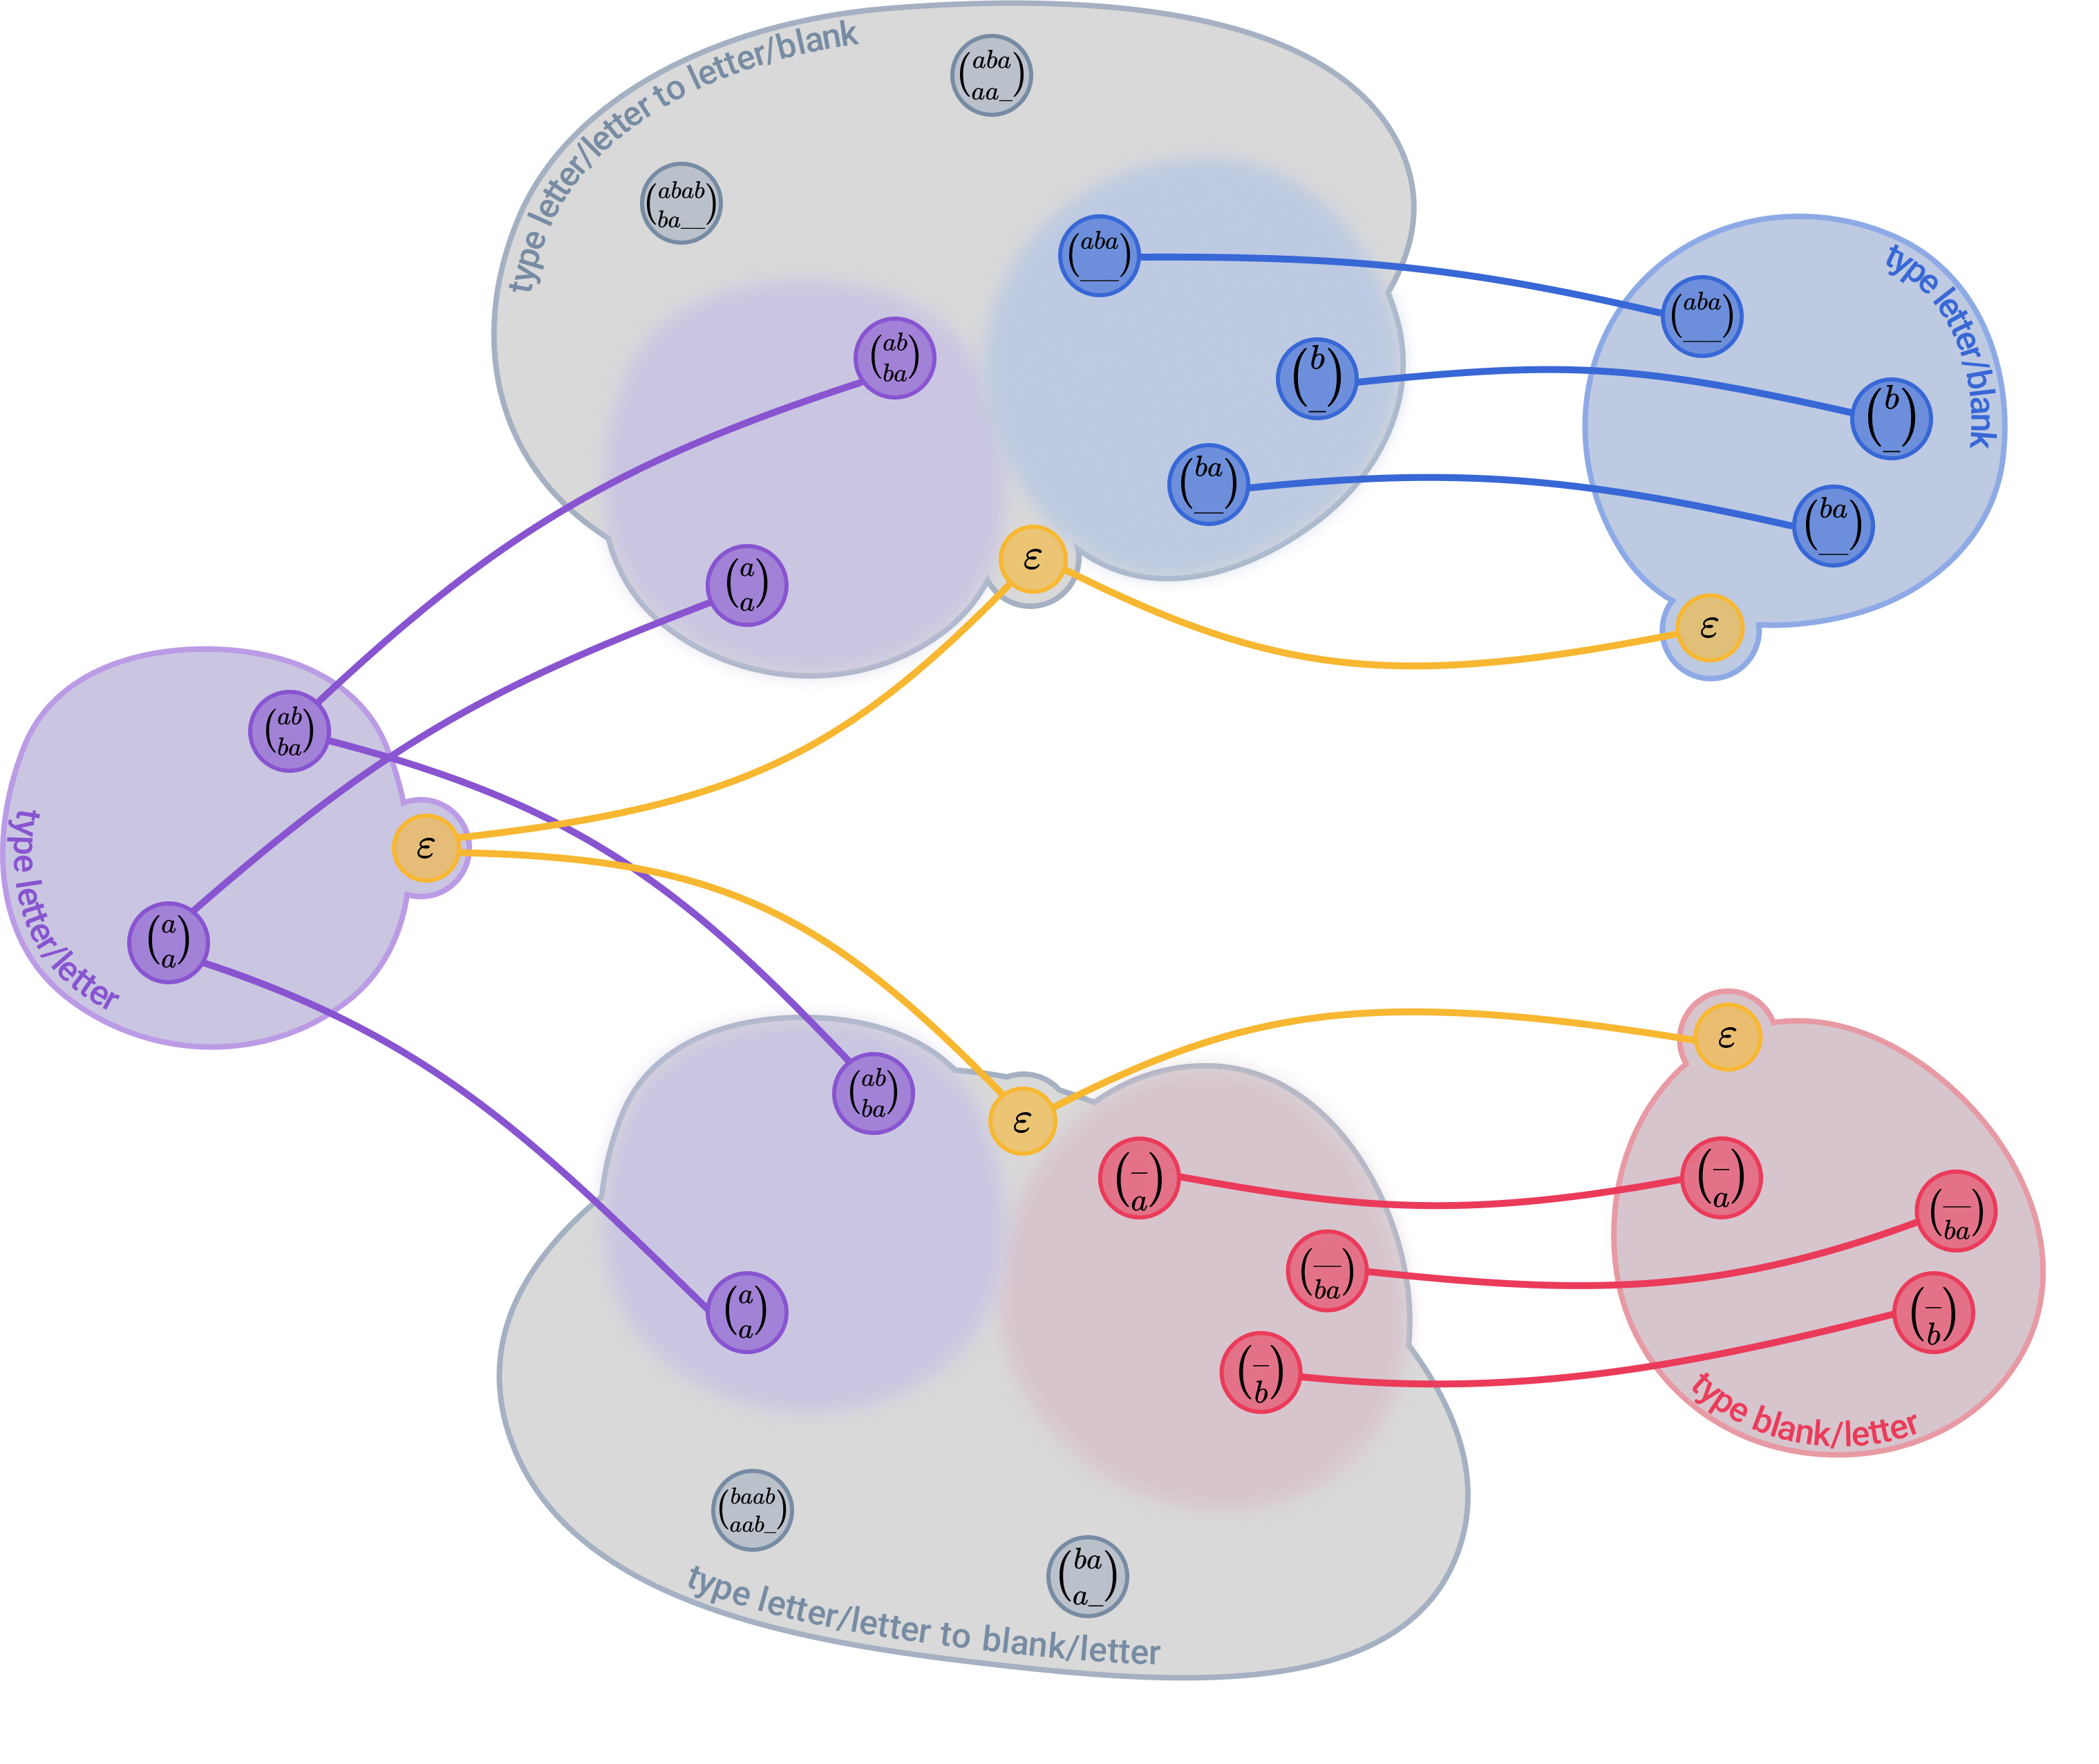
\includegraphics[width=\linewidth]{fig/free_algebras.png}
% 	\caption{My super nice caption.}
% \end{figure}

\begin{table}
	\centering
	\begin{tabular}{cc}
		\toprule
		a & b \\ \midrule
		0 & 1 \\
		1 & 0 \\ \bottomrule
	\end{tabular}
	\caption{My super nice caption.}
\end{table}

\citereset
Hello this is a citation \cite{Bringhurst2005}.
Hello Q\sidenote{Qy first sidenote!} world and another test \cite{Bringhurst2005}.
\[\forall x \in \gamma,\, \exists y\in \delta, \delta \to \gamma\]
\[L \subseteq \Sigma^*\]
\[0 \in \symbb{N}\]
\[\symcal{AbcDefGhiJkl}\]
\[\symscr{AbcDefGhiJkl}\]
\[\symfrak{AbcDefGhiJkl}\]

\lipsum[1-2]

\begin{figure}[htb]
	\centering
	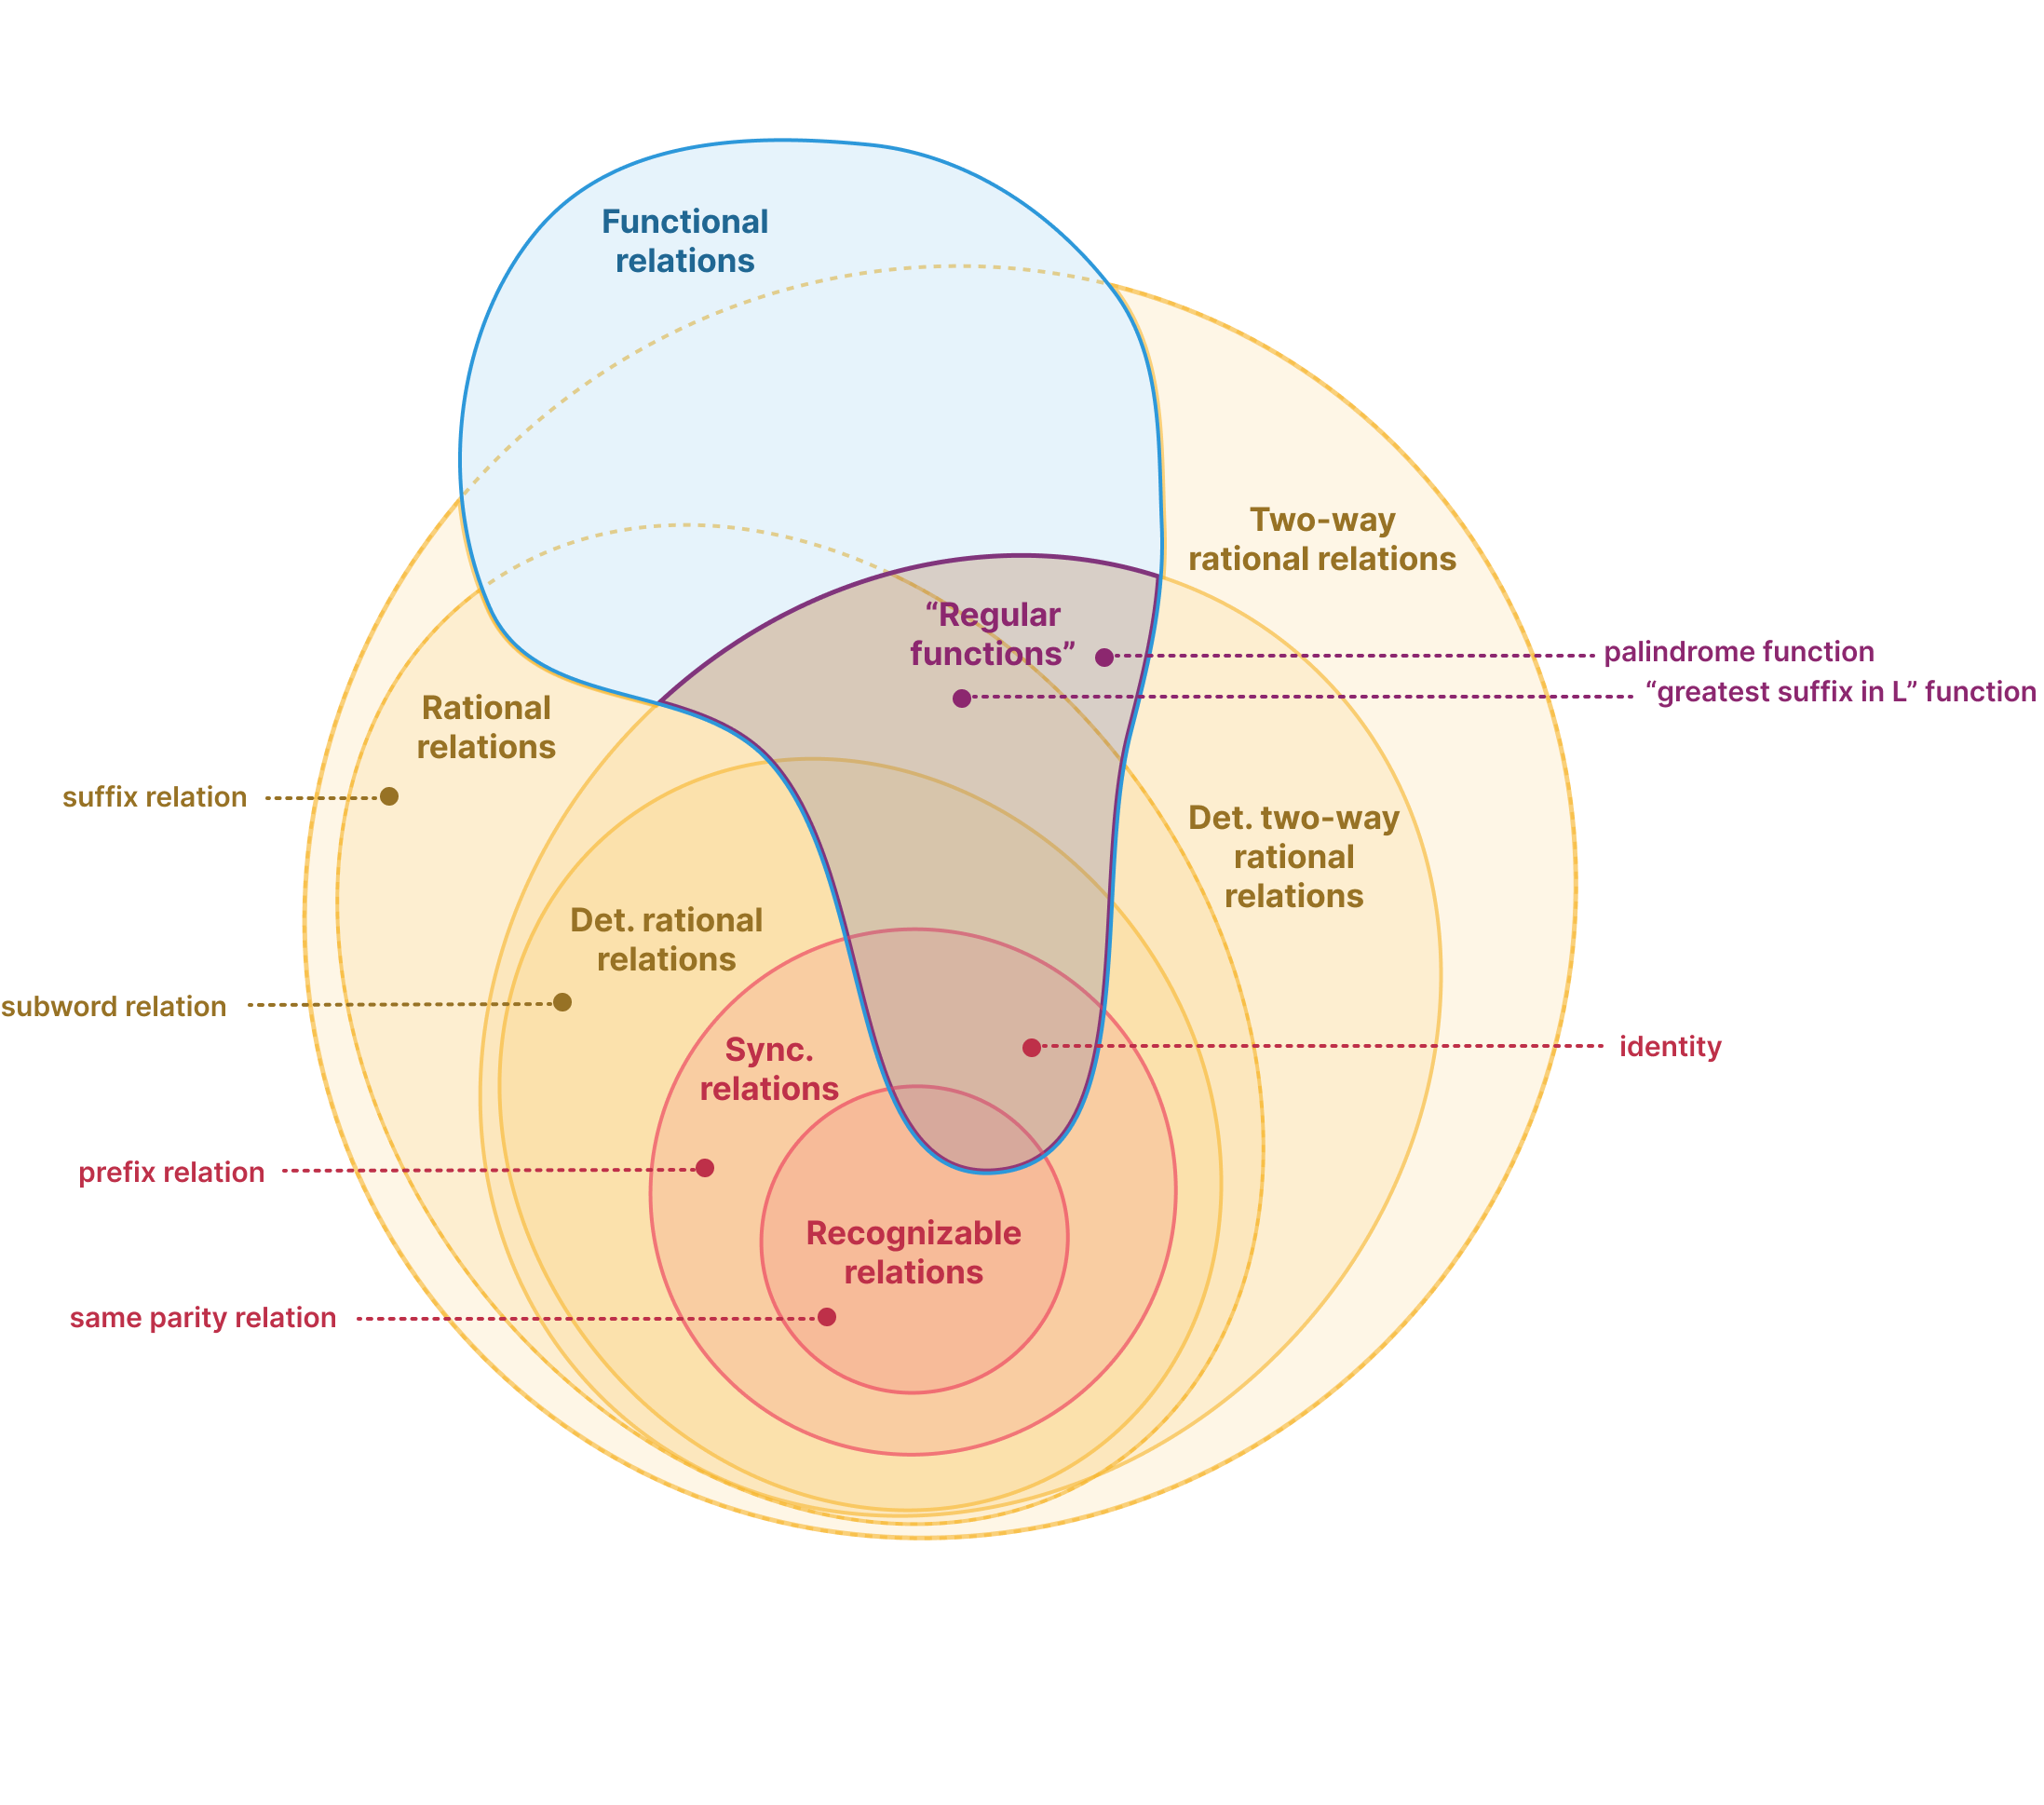
\includegraphics[width=\linewidth]{fig/landscape.png}
	\caption{The landscape of rationality.}
\end{figure}

\lipsum[3-10]

\chapter[Evaluation and Containment of Conjunctive Regular Path Queries]{Evaluation and Containment\\ of Conjunctive Regular Path Queries}

\chapter{Minimization of Conjunctive Regular Path Queries}

\chapter[{Semantic Tree-Width and Path-Width of Conjunctive Regular Path Queries}]{Semantic Tree-Width and Path-Width\\of Conjunctive Regular Path Queries}

% \chapter{Synthesis of Conjunctive Regular Path Queries}

\chapter{Conclusion \& Open Problems}


Extend the notion of `strong minimality` using the axioms used in the lower bound (`str-onto`): call such canonical databases / extensions `structurally minimal'.
Prove or disprove the following result: ``a "CRPQ" has "one-way semantic tree-width" at least $k$ "iff" it has an expansion that is structurally minimal and whose core has tree-width at least $k$''. In general: what about minor-closed classes?
Extend Grohe's Theorem to CRPQs (or maybe to a subclass of CRPQs, "eg" those whose
structurally minimal canonical databases characterize membership to minor-closed classes).

\part[The Frontier of Decidability in Automatic Structures]{The Frontier of Decidability\\in Automatic Structures}

\chapter{%
	\AP\label{ch:preliminaries-automatic-structures}
	Automatic Structures and Synchronous Relations%
}

Should either go to the introduction (general stuff of structures), or prelim of
databases, or here.

\section{Automatic Structures}

\begin{itemize}
	\itemAP padding symbol $\intro*\pad$
	\itemAP convolution of words $\intro*\convol$
	\itemAP convolution of a relation $\intro*\convolRel{\+R}$
	\itemAP ""automatic relation"" and $\intro*\AUT$
	\itemAP domain and relation of a ""presentation"": $\intro*\domainPres{\+A}$ and $\intro*\relPres{\+R}{\+A}$ 
	\itemAP ""automatic structure"" and ""automatic graph""
\end{itemize}

TODO:generalized presentation (non-injective) + effective construction to make them injective.
-> this explains our choice. We avoid the terminology ``regular structure'' because of
``regular graph''.

\section{Stuff Needed in Dichotomy Chapter}

\subsection{First-Order Reduction and First-Order Model Checking}

For the classical notion of \AP""first-order reductions"", see
\cite[Definition 2.11 \& Definition 1.26]{Immerman1998DescriptiveComplexity}.
Note that the complexity of a decision problem is traditionally measured
as a function of the size of the binary encoding of its input.
However, here, the notion of "first-order reductions" deals with
decision problems defined on "relational structures":
\begin{itemize}
	\item any ``classical'' decision problem, "ie" language $L \subseteq \{0,1\}^*$
		can be seen as a class of "structure" over the "signature of binary strings";
	\item for any "relational signature" $\sigma$,
		there is an encoding of "finite $\sigma$-structures" as "finite structures"
		over the "signature of binary strings", "ie" as a ``classical''
		decision problem---see "eg" \cite[\S~2.2]{Immerman1998DescriptiveComplexity}.
\end{itemize}
Importantly, this last encoding is a "first-order reduction", proving that these reductions
make sense not only from a logical perspective, but also from a complexity-theoretic point of
view.

\begin{proposition}[Folklore]
	\label{prop:FO-in-L}
	"FOfin" $\subseteq$ "L".
\end{proposition}

\begin{proof}[Proof sketch]
	The naive recursive algorithm, recursing over the "first-order formula",
	works in logarithmic space: it suffices to keep one pointer to the "structure"
	for every variable of the "formula@@FO", but since this formula is fixed, we only
	require a constant number of pointers.
\end{proof}

Note that usually, "L"-hardness is defined using "first-order reductions".

What we said above work with the implicit assumptions that all structures at hand are 
"finite@@struct". However, part of this can be generalized to "automatic structures"---however, this comes to the cost of losing the inclusion in "L".

\begin{proposition}[Folklore]
	\AP\label{prop:first-order-reduction-preserve-automaticity}
	The image of an "automatic structure" by a "first-order reduction" is
	still an "automatic structure".
\end{proposition}
\begin{proof}
	TODO
\end{proof}

\decisionproblem{""First-Order Model Checking of Automatic Structures""}{
	A "first-order formula" $\phi(x_1,\hdots,x_k)$ over $\sigma$,
	an "automatic presentation" $\•A$ of an "automatic $\sigma$-structure" $\?A$,
	and words $u_1,\hdots,u_k \in \domainPres{\+A}$.
}{
	Does $\?A, u_1,\hdots, u_k \FOmodels \phi$?
}

\begin{proposition}
	\!\footnote{See "eg" \cite[Theorem XII.1.7]{Blumensath2024MSOModelTheory}.}
	%
	\label{prop:first-order-model-checking-automatic-structures}
	"First-order model checking of automatic structures" is decidable in todo.
	Its "data complexity" is "NL"-complete.
\end{proposition}

\begin{proof}
	TODO.

	For the "NL" lower bound, reduction from NFA non-emptiness.
\end{proof}

We define \AP""FOaut"" to be the class of all problems over "automatic structures"
which are "first-order definable". By \Cref{prop:first-order-reduction-preserve-automaticity},
this class is closed under "first-order reductions". Moreover,
by \Cref{prop:first-order-model-checking-automatic-structures}, we obtain an upper bound.

\begin{proposition}
	"FOaut" $\subseteq$ "NL".
\end{proposition}


\subsection{A Model-Theoretic Perspective}

Given an alphabet $\Sigma$, we define on $\Sigma^*$:
\begin{itemize}
	\itemAP a predicate $\intro*\lastLetter{a}$ indicating that the last letter of a word is $a$,
	\itemAP a binary relation $\intro*\equalLength$ indicating that two words have the same length,
	\itemAP a binary relation $\intro*\prefix$ indicating that a word is a prefix of another.
\end{itemize} 
We denote by $\intro*\signatureSynchronous{\Sigma}$ the "signature" $\langle \langle\lastLetter{a}\rangle_{a \in \Sigma},\, \equalLength,\, \prefix \rangle$%
\footnote{For the sake of simplicity, we abusively use the same notations for
the "predicates" and their "interpretations@@predicate" in the "signature".} and
by \AP$\intro*\univStructSynchronous{\Sigma}$ the "$\signatureSynchronous{\Sigma}$-structure" over $\Sigma^*$ where
the "predicates" are "interpreted@@predicate" as above.

\begin{proposition}
	\label{prop:automatic-first-order}
	A relation over $\Sigma^*$ is "automatic@@rel" "iff" it is definable by a "first-order formula" over \(\univStructSynchronous{\Sigma}\).
\end{proposition}

\subsection{Neighbourhoods}

Given a "$\sigma$-structure" $\?A$ and $a \in A$, we define the \AP""neighbourhood"" of $a$
in $\?A$
to be the tuple of sets
\[
	\intro*\neighbourhood{a}{\?A}{\+R}{i} \defeq
	% \Big\langle
		\big\{
			\langle a_1, \hdots, a_{i-1}, a_{i+1}, \hdots, a_k \rangle \in A^{k-1} \mid
			\langle a_1, \hdots, a_{i-1}, a, a_{i+1}, \hdots, a_k \rangle \in \+R(\?A)
		\big\},
		% \;\big\vert\;
		% \+R_{(k)} \in \sigma \text{ and } i \in \lBrack 1,k\rBrack
	% \Big\rangle.
\]
when $\+R$ ranges over "predicate" of arity $k$ of $\sigma$ and $i \in \lBrack 1,k\rBrack$. 
\marginnote{TODO: introduce notation $\+R_{(k)} \in \sigma$}
For "graphs@@dir", the "neighbourhood" of a vertex corresponds to its set of predecessors and
its set of successors.

\begin{proposition}
	\AP\label{prop:neighbourhood-core}
	Given a "$\sigma$-structure" $\?B$, if $\?B$ is a "core", then
	two elements $b_1$ and $b_2$ of $\?B$ have the same "neighbourhood" "iff" $b_1 = b_2$.
\end{proposition}

\begin{proof}
	The right-to-left implication is trivial.
	For the converse one, consider the "homomorphism" from $\?B$ to itself
	which maps $b_2$ to $b_1$, and all elements of $B \smallsetminus \{b_2\}$
	to themselves. Since we assumed that $b_1$ and $b_2$ have the same "neighbourhood",
	this is indeed a "homomorphism", which is clearly not bijective, and
	hence by \Cref{prop:automorphism-core}, $\?B$ is not a "core".
\end{proof}

\subsection{Undirected Paths}

An \AP""undirected path"" in a "$\sigma$-structure" $\?A$ consists of a sequence
\[\big\langle a_0,\, e_0,\, a_1,\, \hdots,\, e_{n-1},\, a_n\big\rangle, \text{ with } n \in \N,\]
where $a_i \in \?A$ and each $e_i$ is a "hyperedge" of $\?A$ "st" both
$a_i$ and $a_{i+1}$ occur in $e_i$. When such an "undirected path" exists, we say that
there is an "undirected path" between $a_0$ and $a_n$, or equivalently
that $a_0$ and $a_n$ are \AP""connected"".%
\sidenote{Note that this defines an equivalence relation.}
A \AP"connected component" of $\?A$ consists of an equivalence class under this relation.

\begin{itemize}
	\itemAP ""incidence graph"" $\intro*\IncidenceGraph{\?A}$, ""distance@@struct"" and ""diameter""
	\itemAP ""simple path""
\end{itemize}
\chapter{A Dichotomy Theorem for Automatic Structures}

\begin{abstract}
	\marginnote[1.3em]{
		TODO: Section X has been published in BLA.

		Part of the dichotomy theorem---Sections X and Y---was proven during the internship
		of Antoine Cuvelier that I supervised in Summer 2024.

		We thank Joanna Fijalkow for helpful discussions on constraint satisfaction problems.
	}%
	We study the separation problem of "synchronous relations", "aka" "synchronous relations",
	by "recognizable relations"---namely finite unions of Cartesian products of "regular languages".
	We prove it to be computationally equivalent to the "finite regular colourability of rational graphs", that takes an "rational presentation" of a "graph" as input, and asks whether
	it admits a "regular colouring"---meaning that for each colour, the set of words representing the elements having this colour is a "regular language"---with finitely many colours.

	We first show that, if the number of colours is fixed to be any natural number $k \geq 2$, then
	this problem is undecidable. This implies the undecidability of the separation problem
	of "synchronous relations" by "recognizable relations" where the number of unions allowed is bounded.

	We then generalize this result, and prove a dichotomy theorem for automatic structures:
	for any "relational structure" $\?B$, the problem of whether an "automatic structure"
	admits a "homomorphism" to $\?B$ is either decidable in "NL", or is undecidable.
	We extend these results to "regular homomorphisms", for which we require the "homomorphisms"
	to be "regular@@hom", in the sense that every preimage of any element of the "target structure" $\?B$ must be a "regular language". In both cases, "structures" for which the problem is 
	decidable are those with ``"finite duality"''. 
	
	Using this dichotomy theorem, we then prove that the original problem, 
	namely the separation problem of "synchronous relations"
	by "recognizable relations" is undecidable.
\end{abstract}
\clearpage
\chaptertoc
\clearpage

\cite[Test]{Atserias2008DigraphColoring}
\cite{Atserias2008DigraphColoring}
\cite{Atserias2008DigraphColoring}

% \lipsum[1]
% \citemain[Test]{Atserias2008DigraphColoring}

% \lipsum[1]
% \footnote{Test: \citeside[Definition 2.11 \& Definition 1.26]{Immerman1998DescriptiveComplexity}. \simplecite{Immerman1998DescriptiveComplexity}}

Let \AP$\intro*\Fin$ denote the class of all "finite $\sigma$-structures",
\AP$\intro*\Aut$ the class of all "automatic $\sigma$-structures".
We let \AP$\intro*\AutPres$ be the class of all "rational presentations of $\sigma$-structures",
and \AP$\intro*\FinPres$ be the subclass of "presentations" of "finite $\sigma$-structures".

We denote by \AP$\intro*\HomFinClass{\?B}$ and $\intro*\HomAllClass{\?B}$ the class
of all finite (resp. all) "$\sigma$-structures" that admit a "homomorphism" to $\?B$.

Given a "$\sigma$-structure" $\?B$, and a class $\classStruct$ of "rational presentations of $\sigma$-structures", we denote by \AP$\intro*\HomDec{\classStruct}{\?B}$ the class of all presentations $\•A \in \classStruct$ such that the "$\sigma$-structure" $\?A$
that they "represent@@structure" admits a "homomorphism" to $\?B$.
Similarly, we denote by \AP$\intro*\HomRegDec{\classStruct}{\?B}$ the class 
associated to "regular homomorphisms".%
\sidenote{Todo: set-theoretic bullshit. Not a set but it is if we fix an alphabet. Blabla.}

While the existence of a "homomorphism" from some "rational presentation" of $\?A$ 
to a "finite $\sigma$-structure" $\?B$ only depends on $\?A$ and not the "presentation" itself,
this is not true for "regular homomorphism".
For a $\sigma$-structure $\?B$,
we use \AP$\intro*\HomFinDec{\?B}$, $\intro*\HomAutDec{\?B}$, $\intro*\HomRegFinDec{\?B}$
and $\intro*\HomRegAutDec{\?B}$ as shorthands for $\HomDec{\FinPres}{\?B}$, $\HomDec{\AutPres}{\?B}$,
$\HomRegDec{\FinPres}{\?B}$ and $\HomRegDec{\AutPres}{\?B}$, respectively.

Note that any "homomorphism" from an "rational presentation" of a "finite structure"
to a "finite structure" is also "regular@@hom" and so $\HomFinDec{\?B} = \HomRegFinDec{\?B}$.\sidenote{Note also that membership in $\HomFinDec{-} = \HomRegFinDec{-}$ and in
$\HomAutDec{-}$ only depends on the "structure represented"
by the "rational presentation", and not on the "presentation" itself.
This is not the case for $\HomRegAutDec{-}$. We use these definitions for two reasons: (1) for consistency with $\HomRegAutDec{-}$ and (2) for the associated decision problem to be defined unambiguously. Note moreover that in the case of "finite structures", the size of its representation, say using adjacency lists, and of its "rational presentation" are equal up to a TODO}

\section{\AP\label{sec:dichotomy-introduction}%
	Introduction}

\begin{restatable*}{theorem}{DichotomyThmDichotomyAutomatic}[Dichotomy Theorem for Automatic Structures]
	\!\footnote{The equivalence between (1) and (2) still holds
	when the "homomorphism problem" takes as input ``higher-order automatic
	structures'' as defined in \cite[last remark of \S~XII.3]{Blumensath2024MSOModelTheory},
	since such structures have a decidable first-order theory.}%
	%%%
	\AP\label{thm:dichotomy-theorem-automatic-structures}
	Let $\?B$ be an arbitrary "$\sigma$-structure". The following are equivalent:
	\begin{description}
		\itemAP[\intro*\itemDTFinDual.] $\?B$ has "finite duality";
		\itemAP[\intro*\itemDTHomDec.] $\HomAutDec{\?B}$ is decidable;
		\itemAP[\intro*\itemDTHomRegDec.] $\HomRegAutDec{\?B}$ is decidable;
		\itemAP[\intro*\itemDTEqual.] $\HomAutDec{\?B} = \HomRegAutDec{\?B}$ "ie" for any "rational presentation" $\•A$ of a 
		"$\sigma$-structure" $\?A$, there is a "homomorphism" from $\?A$ to $\?B$ "iff" 
		there is a "regular homomorphism" from $\•A$ to $\?B$;
		\itemAP[\intro*\itemDTFirstOrder.] $\HomAllClass{\?B}$ has "uniformly first-order definable homomorphisms".
	\end{description}
	Moreover, when $\HomAutDec{\?B}$ and $\HomRegAutDec{\?B}$ undecidable, they are "coRE"-complete
	and "RE"-complete, respectively. When they are decidable, they are "NL".
\end{restatable*}
	  
TODO: say that to have "finite duality" can be decided.
\section{\AP\label{sec:dichotomy-preliminaries}%
	Preliminaries}

\subsection{Constructions on Structures}

Given two "structures" $\?A$ and $\?B$, we define the structure \AP$\intro*\powstruct{\?B}{\?A}$ as follows:
\begin{itemize}
  \item its domain are "homomorphisms" $\?A \to \?B$,
  \item for every "predicate" $\+R$ of arity $k$, for any homomorphism $f_1,\hdots,f_k$,
  we have $\langle f_1,\hdots,f_k\rangle \in \+R$ when for every
  $\langle a_1,\hdots,a_k\rangle \in \+R(\?A)$
  then $\langle f_1(a_1), \hdots, f_k(a_k) \rangle \in \+R(\?B)$.
\end{itemize}


\begin{proposition}[Folklore: Currying Homomorphisms]
	\AP\label{prop:currying-hom}
	Given "structures" $\?A$, $\?B$ and $\?C$, if $f\colon \?A\prodstruct \?B \to \?C$
	is a "homomorphism", then $F\colon \?A \to \powstruct{\?C}{\?B}$,
	defined by $a \mapsto (b \mapsto f(a,b))$, is a "homomorphism".
	In fact, this mapping $f \mapsto F$ is a bijection
	between "homomorphisms" $\?A\prodstruct \?B \to \?C$
	and "homomorphisms" $\?A \to \powstruct{\?C}{\?B}$.
\end{proposition}

\begin{proof}
Let $\+R$ be a predicate of arity $k$, and let
$\langle a_1,\hdots,a_k \rangle \in \+R(\?A)$.
We want to show that $\langle F(a_1),\hdots,F(a_k) \rangle \in \+R(\powstruct{\?C}{\?B})$:
for any $\langle b_1,\hdots,b_k \rangle \in \+R(\?B)$, we have
\[\langle F(a_1)(b_1), \hdots, F(a_k)(b_k)\rangle = \langle f(a_1,b_1),\hdots,f(a_k,b_k) \rangle \in \+R(\?C)\] since $f$ is a "homomorphism" from $\?A\prodstruct \?B$ to $\?C$.
Hence, $F$ is indeed a "homomorphism" from $\?A$ to $\powstruct{\?C}{\?B}$.

Dually, if $F$ is a "homomorphism" from $\?A$ to $\powstruct{\?C}{\?B}$,
we define $f\colon \?A\prodstruct \?B \to \?C$ by $\langle a,b \rangle \mapsto F(a)(b)$,
and claim that $f$ is a "homomorphism". Indeed, if $\+R$ be a predicate of arity $k$,
for any $\langle a_1, \hdots, a_k \rangle \in \+R(\?A)$
and $\langle b_1, \hdots, b_k \rangle \in \+R(\?B)$,
we have $\langle f(a_1,b_1), \hdots, f(a_k,b_k) \rangle
= \langle F(a_1)(b_1), \hdots, F(a_k)(b_k) \rangle$.
Since $\langle F(a_1), \hdots, F(a_k) \rangle \in \+R(\powstruct{\?C}{\?B})$
and $\langle b_1, \hdots,b_k \rangle \in \+R(\?B)$ 
it follows that $\langle F(a_1)(b_1), \hdots, F(a_k)(b_k) \rangle \in \+R(\?C)$.
Therefore, $f$ is a "homomorphism" from $\?A \prodstruct \?B$ to $\?C$.

It is then routine to check that the maps $f \mapsto F$ and $F \mapsto f$ defined
in the two previous paragraphs are mutually inverse bijections.
\end{proof}

\subsection{Constructions on rational presentations}
\label{sec:construction-automatic-presentations}

Let $\•A$ and $\•B$ be "rational presentations" of some "$\sigma$-structures"
$\?A$ and $\?B$. We define \AP$\•A \intro*\prodpres \•B$ to be the "presentation@@auto"
"st":
\begin{align*}
	\domainPres{\•A\prodpres \•B} & \defeq \{u\#v \mid u \in \domainPres{\•A} \land v \in \domainPres{\•B}\}\\
	\relPres{\•A\prodpres \•B}{\+R} & \defeq \{(u_1\#v_1) \convol \cdots \convol (u_k\#v_k) \mid
		u_1 \convol \cdots \convol u_k \in \relPres{\•A}{\+R} \land
		v_1 \convol \cdots \convol v_k \in \relPres{\•B}{\+R}
	\}
\end{align*}
for each "predicate" $\+R$ of arity $k$ in $\sigma$.
It is an "rational presentation" of $\?A \prodstruct \?B$. TODO:proof.

\begin{proposition}
	\label{prop:homreg-prod-finite}
	Let $\?A$, $\?B$ and $\?C$ be "automatic $\sigma$-structures", such that
	$\?B$ and $\?C$ are finite.
	Let $\•A$ (resp. $\•B$ and $\•B'$, resp. $\•C$ and $\•C'$) be an "rational presentation"
	of $\?A$ (resp. $\?B$, resp. $\?C$).
	Then $\•A \prodpres \•B \homregto \•C$ "iff" $\•A \prodpres \•B' \homregto \•C'$.
\end{proposition}

\begin{proof}
	The proof will follow from the following claim.
	\begin{claim}
		\label{claim:homreg-prod-finite}
		A function $f\colon\•A \prodpres \•B \homregto \•C$ is a "regular homomorphism"
		"iff" for every $b\in \domainPres{\•B}$, for every $c\in \domainPres{\•C}$,
		\(\{
			a\in \domainPres{\•A} \mid f(a,b) = c
		\}\)
		is a "regular language".
	\end{claim}
	TODO.
\end{proof}

In other words, the existence of a "regular homomorphism" does not depend on the
"rational presentation" of the \emph{finite} "structures" that are involved, but only
on the "structure" they represent.
As a consequence of \Cref{prop:homreg-prod-finite}, we write
\(\•A \prodpres \?B \homregto \?C\) as a synonym for \(\•A \prodpres \•B \homregto \•C\).

\begin{corollary}[Currying]
	\label{coro:homreg-currying}
	Let $\?A$, $\?B$ and $\?C$ be "automatic $\sigma$-structures",
	and let $\•A$ be an "rational presentation" of $\?A$.
	Then $\•A \prodpres \?B \homregto \?C$ "iff" $\•A \homregto \powstruct{\?C}{\?B}$.
\end{corollary}

\begin{proof}
	By \Cref{claim:homreg-prod-finite}… TODO.
\end{proof}

\subsection{Idempotent Core}

We fix a "purely relational signature" $\sigma$.
Given a "$\sigma$-structure" $\?B$,
we denote by \AP$\intro*\extendedSignature{\sigma}{\?B}$
the signature obtained from $\sigma$ by adding
a unary predicate \AP$\intro*\unarypred{b}$ for each $b\in B$.
The \AP""marked structure"" \AP$\intro*\marked{\?B}$ of $\?B$ is the
"$\extendedSignature{\sigma}{\?B}$-structure"
obtained from $\?B$ by "interpreting@@predicate" each predicate $\unarypred{b}$ as the
singleton $\{b\}$.\sidenote{TODO: ASIA'S REMARK: this is called the ``idempotent core''.}

\begin{proposition}[Folklore]
\!\sidenote{The non-easy part is to reduce $\HomFinDec{\marked{\?B}}$ to $\HomFinDec{\?B}$: only this reduction
requires the assumption that $\?B$ is a core. This reduction is folklore, see "eg"
\autocite[Lemma 2.5]{LaroseTesson2009UniversalAlgebraCSP}.
TODO: understand if the proof is indentical to us. We provide here a self-contained proof.}%
\sidenote{The "marked structure" $\marked{\core{\?B}}$ of the "core" of $\?B$ is
usually called the \AP""idempotent core""
of $\?B$. By TODO:addref and this proposition, $\HomFinDec{\?B}$ and
$\HomFinDec{\marked{\core{\?B}}}$ are equivalent under "first-order reductions".
This reduction is a central tool
in the algebraic approach to understand "constraint satisfaction
problem" since the algebra associated to the "CSP" over an "idempotent core"
only has idempotent operations, making it much easier to work with. See TODO:addref for
more details.}%
\AP\label{prop:marking-preserves-csp-complexity}
If $\?B$ is a finite "core", then the problems $\HomFinDec{\marked{\?B}}$ and 
$\HomFinDec{\?B}$ are equivalent under "first-order reductions".
\end{proposition}

\begin{proof}[Proof of \Cref{prop:marking-preserves-csp-complexity}]
\proofcase{Reduction from $\HomFinDec{\?B}$ to $\HomFinDec{\marked{\?B}}$.}
We reduce a "$\sigma$-structure" $\?A$ to the
"$\extendedSignature{\sigma}{\?B}$-structure" $\?A'$ obtained
from $\?A$ by "interpreting@@predicate" each predicate $\unarypred{b}$ as the emptyset.
Clearly, a function from $A$ to $B$ is a "homomorphism" from $\?A$ to $\?B$
"iff" it is a "homomorphism" from $\?A'$ to $\marked{\?B}$, proving the correctness
of the reduction. It is, by definition, "first-order@@reduction".

\proofcase{Reduction from $\HomFinDec{\marked{\?B}}$ to $\HomFinDec{\?B}$.}
We first define the reduction $\Phi$ and show its correctness, we will show later that it
is a "first-order reduction". We reduce a "$\extendedSignature{\sigma}{\?B}$-structure" $\?A$ to the "$\sigma$-structure"
$\Phi(\?A)$ defined as follows:
\begin{itemize}
	\item its underlying universe is the disjoint union $A \dcup B$,
	\item given a "predicate" $\+R$ of arity $k$, its "hyperedges" are:
	\begin{itemize}
	\item all $\+R$-"hyperedges" of $A$,
	\item all $\+R$-"hyperedges" of $B$, and
	\item all $\+R$-"hyperedges" $(b_1,\hdots,b_{i-1}, a_i, b_{i+1},\hdots,b_k)$
		"st" there exists $b_i$ for which the $\+R$-"hyperedge"
		$(b_1,\hdots,b_{i-1}, b_i, b_{i+1},\hdots,b_k)$
		is in $\+R(\?A)$, and $a_i$ belongs to the "interpretation@@predicate" of 
		$\unarypred{b_i}$ in $\?A$.
	\end{itemize}
\end{itemize}
Note that by construction, the "neighbourhood" of $a \in A$ in $\Phi(\?A)$ is
the union of its "neighbourhood" in $\?A$, and the union of the "neighbourhoods" of
$b$ in $\?B$ for all $b$ "st" $a \in \unarypred{b}(\?A)$.
TODO: To be concluded.  
\end{proof}

\subsection{Transitive Tournaments "vs" Paths}

\begin{figure}
	\centering
	\begin{tikzpicture}
		\node[vertex] (0) at (0,0) {};
\node[vertex, below right=of 0] (1) {};
\foreach \i in {1, 3, 5, 7, 9} {
	\pgfmathtruncatemacro{\next}{\i + 1}
	\pgfmathtruncatemacro{\nnext}{\i + 2}
	\node[vertex, below right=of \i] (\next) {};
	\node[vertex, above right=of \next] (\nnext) {};
};
\node[vertex, below right=of 11] (12) {};
\node[vertex, below right=of 12] (13) {};

% ---
% Transitions
% ---
\foreach \i in {0,1,3,5,7,9,11,12} {
	\pgfmathtruncatemacro{\next}{\i + 1}
	\draw[edge] (\i) to (\next);
};
\foreach \i in {2,4,6,8,10} {
	\pgfmathtruncatemacro{\next}{\i + 1}
	\draw[edge] (\next) to (\i);
}
		
\foreach \i in {1,3,5,7,9,11} {
	\pgfmathtruncatemacro{\half}{\i / 2}
	\node[draw=none, above right=-.6em of \i] {$a_{\half}$};
};
\foreach \i in {2,4,6, 8, 10, 12} {
	\pgfmathtruncatemacro{\half}{(\i / 2) - 1}
	\node[draw=none, below left=-.6em of \i] {$b_{\half}$};
};
\node[draw=none, below left=-.6em of 0] {$a'_0$};
\node[draw=none, above right=-.6em of 13] {$b'_5$};

\draw[decoration={brace}, decorate, transform canvas={yshift=1.5em}] (3.north west) to node[midway, above] {$\+O(n)$ nodes} (11.north east);
	\end{tikzpicture}
	\caption{\AP\label{fig:zigzag-graph}The "zigzag graph" $\zigzag{5}{2}$.}
\end{figure}
\begin{example}
	\AP\label{ex:zigzag-defn}
	Let $n\in\?N$.
	We define the \AP""zigzag graph"" $\intro*\zigzag{n}{2}$ of width $n$ and length 2
	to be "graph" whose vertices are $a_0, \hdots, a_n$, $b_0, \hdots, b_{n}$,
	$a'_0$ and $b'_n$, with edges from $a_i$ to $b_{i-1}$ and to $b_{i}$ (for $i \in \lBrack 0,n\rBrack$, whenever the nodes exist), and with an edge from $a'_0$ to $a_0$ and from $b_n$
	to $b'_n$. See \Cref{fig:zigzag-graph} for an illustration.
	
	Note that $\zigzag{n}{2}$ does not admit a "homomorphism" to the "$2$-path"---indeed, such a homomorphism should send $a'_0$, $a_0$ and $b_0$ onto $0$, $1$, and $2$, respectively, 
	and so all $a_i$'s (resp. $b_i$'s) must be sent onto $1$ (resp. $2$), but then $b'_n$ cannot be mapped anywhere.

	On the other hand, $\zigzag{n}{2}$ admits a "homomorphism" to the "$2$-transitive tournament", as witnessed by \Cref{fig:zigzag-graph-hom-T2}.
	In fact, this "homomorphism" is far from being unique:
	each vertex $a_1,\,a_2,\,\hdots,\,a_{n-1}$ can be sent on either $0$ or $1$
	(the red and purple vertices), 
	and similarly, each vertex $b_1,\,b_2,\,\hdots,\,b_{n-1}$ can be sent on either $1$ or $2$
	(the purple and blue vertices).\footnote{Note that it is straightforward
	to extend these results---namely $\zigzag{n}{2} \homto \transitiveTournament{2}$
	and $\zigzag{n}{2} \nothomto \pathGraph{2}$---to arbitrary values of $k\in \N$ with
	$k\geq 2$, namely $\zigzag{n}{k} \homto \transitiveTournament{k}$
	and $\zigzag{n}{k} \nothomto \pathGraph{k}$, by letting
	$\zigzag{n}{k}$ be the graph obtained from $\zigzag{n}{2}$ by
	replacing the path leading to $a_0$ by a path of length $k-1$.
	}
\end{example}
\begin{figure}
	\centering 
	\begin{tikzpicture}
		\node[vertex, draw=c0, fill=c0, fill opacity=.4] (0) at (0,0) {};
\node[vertex, below right=of 0, draw=c1, fill=c1, fill opacity=.4] (1) {};
\foreach \i in {1, 3, 5, 7, 9} {
	\pgfmathtruncatemacro{\next}{\i + 1}
	\pgfmathtruncatemacro{\nnext}{\i + 2}
	\node[vertex, below right=of \i, draw=c2, fill=c2, fill opacity=.4] (\next) {};
	\node[vertex, above right=of \next, draw=c0, fill=c0, fill opacity=.4] (\nnext) {};
};
\node[vertex, below right=of 11, draw=c1, fill=c1, fill opacity=.4] (12) {};
\node[vertex, below right=of 12, draw=c2, fill=c2, fill opacity=.4] (13) {};

% ---
% Transitions
% ---
\foreach \i in {0,1,3,5,7,9,11,12} {
	\pgfmathtruncatemacro{\next}{\i + 1}
	\draw[edge] (\i) to (\next);
};
\foreach \i in {2,4,6,8,10} {
	\pgfmathtruncatemacro{\next}{\i + 1}
	\draw[edge] (\next) to (\i);
}

% ---
% 2-transitive tournament
% ---
\node[vertex, above right=-.25em and 5em of 13, draw=c2, fill=c2, fill opacity=.4] (t2-2) {};
\node[vertex, above=of t2-2, draw=c1, fill=c1, fill opacity=.4] (t2-1) {};
\node[vertex, above=of t2-1, draw=c0, fill=c0, fill opacity=.4] (t2-0) {};

\draw[edge] (t2-0) to (t2-1) to (t2-2);
\draw[edge] (t2-0) to[bend left=60] (t2-2);
	\end{tikzpicture}
	\caption{\AP\label{fig:zigzag-graph-hom-T2}A "homomorphism" from the "zigzag graph" (left-hand side) to the "$2$-transitive tournament" (right-hand side).}
\end{figure}
\section{%
	\AP\label{sec:dichotomy-colouring}%
	From Separation to Colouring of Automatic Graphs
}

\subsection{Separability is Equivalent to Regular Colourability}

We start by showing that the "separability problem" in terms of arbitrary "recognizable relations" is equivalent, under polynomial time reductions, 
to the "regular colourability problem". To make our statement precise, we need some terminology introduced below. 
\AP
Let $\intro*\kREC$ be the class of languages expressed by unions of products of $k$ regular languages which form a partition, that is (in the binary case), relations of the form $(L_{i_1} \times L_{j_1}) \cup \dotsb \cup (L_{i_\ell} \times L_{j_\ell})$, with $i_1,j_1,\hdots,i_\ell, j_\ell \in \lBrack 1,k \rBrack$, for some regular partition $L_1, \dotsc, L_{k}$ of $\Sigma^*$ and $\ell \in \N$.
\AP
Note that $\REC = \bigcup_k \kREC$.
\AP%
Let us denote by $\intro*\Id$ the identity relation (on any implicit alphabet). Observe that $\Id$ is "automatic" but not "recognizable".

\begin{theorem}
    \AP\label{thm:reg-colourability-equiv-separability}
    There are polynomial-time reductions: 
    \begin{enumerate}
        \item from the "$\REC$-separability problem" to the "regular colourability problem"; 
        \item from the "regular colourability problem" to the "$\REC$-separability problem"; and
        \item from the "$k$-regular colourability problem" to the $\kREC$-"separability problem", for every $k > 0$.
    \end{enumerate}
    Further, the last two reductions are so that the second relation in the instance of the "separability problem" is the identity $\Id$.
\end{theorem}
   
\begin{proof}
   We start with the last two reductions.
    Given an "automatic graph" $\AutGraph{L}{E}$ over an alphabet $\Sigma$, consider the instance $R_1,R_2$ for the $\REC$-"separability problem", where 
    $R_1 = E$ and $R_2 = \Id$. 
    %
    If $\AutGraph{L}{E}$ is "$k$-regular colourable" via the colouring $V_1, \dotsc, V_k$ then the $\kREC$ relation
    $\bigcup_{i \neq j} V_i \times V_j$ separates $R_1$ and $R_2$.
    %
    Conversely, if a $\kREC$ relation $R \subseteq \Sigma^* \times \Sigma^*$ on the partition $V_1 \dcup \dotsb \dcup V_k = \Sigma^*$ separates $R_1$ and $R_2$, then $\bigcup_{i \neq j} V_i \times V_j$ also separates $R_1$ and $R_2$, and this implies that $V_1, \dotsc, V_k$ is a $k$-colouring for $\AutGraph{\Sigma^*}{E}$.
%\end{proof}

\AP For the first reduction, let us introduce some terminology.
Given two relations $R_1,R_2$ over $\Sigma^*$, say that $u \in \Sigma^*$ is ""compatible"" with
$u' \in \Sigma^*$ when for all words $v \in \Sigma^*$:
\begin{center}
    \intro*\compL: $(u,v) \in R_1 \Rightarrow (u',v) \not\in R_2$%
    ,\hphantom{\quad and \quad}
    \intro*\compR: $(v,u) \in R_1 \Rightarrow (v,u') \not\in R_2$,\\
    \intro*\compLpr: $(u',v) \in R_1 \Rightarrow (u,v) \not\in R_2$%
    \hphantom{,}\quad and \quad
    \intro*\compRpr: $(v,u') \in R_1 \Rightarrow (v,u) \not\in R_2$.
\end{center}
\AP
Define the ""incompatibility graph"" $\intro*\incompGraph{R_1}{R_2}$
as the graph whose vertices are all words of $\Sigma^*$,
and with an edge from $u$ to $v$ whenever $u$ is not "compatible" with $v$.
Note that $\incompGraph{R}{\Id}$ is exactly the graph $\AutGraph{\Sigma^*}{R}$.

\begin{example}
    \AP\label{ex:equal-length-plusone}%
    \begin{marginfigure}%
        \centering
        \begin{tikzpicture}
            \input{tikz/dichotomy/ex-R2}
        \end{tikzpicture}
        \caption{\AP\label{fig:equal-length-plusone-relation}%
            The relation $R_2$ of \Cref{ex:equal-length-plusone},
            restricted to words of length at most 2.
        }
    \end{marginfigure}%
    \begin{marginfigure}%
        \centering
        \begin{tikzpicture}
            \input{tikz/dichotomy/ex-Inc}
        \end{tikzpicture}
        \caption{\AP\label{fig:equal-length-plusone-incompatibility}%
            Incompatibility graph $\incompGraph{R_1}{R_2}$ and its "2-regular coloring".%
        }
    \end{marginfigure}%
    Let $\Sigma = \{a,b\}$, $R_1$ be the equal-length relation,
    and
    \[
        R_2 = \{(u, ua) \mid u \in \Sigma^*\} \cup \{(u, ub) \mid u \in \Sigma^*\}.
    \]
    Then, $u$ is "incompatible" with $u'$ if $|u| = |u'|+1$ (this is given by \compL~or \compR),
    or if $|u'| = |u|+1$ (this is given by \compLpr~or \compRpr).
    $R_2$ and the "incompatibility graph" are depicted in \Cref{fig:equal-length-plusone-relation,fig:equal-length-plusone-incompatibility}.
    
    Note that $R_1$ and $R_2$ are separable by the "recognizable" relation
    $S$ consisting of all pairs $(u,v)$ such that $|u|$ and $|v|$ have the same parity.
    Moreover, $\incompGraph{R_1}{R_2}$ is "2-regular colorable", the two colors being
    the words of even and odd length.
\end{example}

\begin{lemma}
    \AP\label{lem:incomp-is-automatic}
    If $R_1$ and $R_2$ are "automatic", then so is $\incompGraph{R_1}{R_2}$.
    Moreover, we can build an automaton for $\incompGraph{R_1}{R_2}$ in polynomial time in the size of the automata for $R_1$ and $R_2$.
\end{lemma}

\begin{proof}
    By definition, the "incompatibility relation" $\incompGraph{R_1}{R_2}$ can be written as
	$R_{\neg\compL} \cup R_{\neg\compLpr} \cup R_{\neg\compR} \cup R_{\neg\compRpr}$, where:
	\begin{align*}
        R_{\neg\compL} &\defeq \big\{ (u,u') \in \Sigma^* \times \Sigma^* \;\big\vert\; \exists v \in \Sigma^*,\; (u,v) \in R_1 \land (u',v) \in R_2 \big\} \text{,}\\
        R_{\neg\compLpr} &\defeq \big\{ (u,u') \in \Sigma^* \times \Sigma^* \;\big\vert\; \exists v \in \Sigma^*,\; (u',v) \in R_1 \land (u,v) \in R_2 \big\} \text{,}\\
        R_{\neg\compR} &\defeq \big\{ (u,u') \in \Sigma^* \times \Sigma^* \;\big\vert\; \exists v \in \Sigma^*,\; (v,u) \in R_1 \land (v,u') \in R_2 \big\} \text{, and}\\
        R_{\neg\compRpr} &\defeq \big\{ (u,u') \in \Sigma^* \times \Sigma^* \;\big\vert\; \exists v \in \Sigma^*,\; (v,u') \in R_1 \land (v,u) \in R_2 \big\}
    \end{align*}
    % % \end{itemize}
    % \begin{itemize}
    %     \item $\neg$\compL:  $(u,v) \in R_1$ and $(u',v) \in R_2$, or
    %     \item $\neg$\compLpr: $(u',v) \in R_1$ and $(u,v) \in R_2$, or
    %     \item $\neg$\compR: $(v,u) \in R_1$ and $(v,u') \in R_2$, or
    %     \item $\neg$\compRpr: $(v,u') \in R_1$ and $(v,u) \in R_2$.
    % \end{itemize} 
    Observe that starting from automata for $R_1$ and $R_2$, then for each
	of the relation $R_{\neg\compL}$, $R_{\neg\compLpr}$, $R_{\neg\compR}$ or $R_{\neg\compRpr}$, we can build an automaton recognizing them
	using a product construction, which can be implemented in polynomial time.
    % as follows:
    % \begin{itemize}
    %     \item its states are $Q_1 \times Q_2$;
    %     \item for each transition $q_1 \xrightarrow{(a,b)} q'_1$ in $\+A_1$
    %         and each transition $q_2 \xrightarrow{(c,b)} q'_2$ in $\+A_2$,
    %         put a transition $(q_1,q_2) \xrightarrow{(a,c)} (q'_1,q'_2)$,
    %         with $a,b,c \in \A\cup\{\bot\}$;\footnote{Potentially, this
    %         could produced transition labelled by $(\bot,\bot)$: we can get rid of those
    %         using the standard elimination of $\varepsilon$-transitions.}
    %     \item a state $(q_1,q_2)$ is accepting if $q_1$ and $q_2$ are accepting
    %         in $\+A_1$ and $\+A_2$, respectively.
    % \end{itemize}
    It then follows that we can build a polynomial automaton recognizing
    $\incompGraph{R_1}{R_2}$.
\end{proof}

%\begin{proposition}
%    \AP\label{prop:sep-to-col-reduction}
%    There is a polynomial-time reduction
%    from the $\REC$-"separability problem" to the 
%    "regular colourability problem" on "automatic graphs".
%\end{proposition}

%\begin{proof}
    \AP Given an instance $(R_1,R_2)$ of the "separability problem", we
    reduce it to the "regular colourability problem" on its "incompatibility graph" $\incompGraph{R_1}{R_2}$.

    \proofcase{Left-to-right implication:} 
   Assume that there exists $S$ in $\kREC$ that "separates" $R_1$ from $R_2$.
   %, where each $A_i$ and $B_i$ is regular.
    Then $S$ can be written as $(A_{i_1}\times A_{j_1}) \cup \cdots \cup (A_{i_\ell}\times A_{j_\ell})$, 
    where $(A_1,\hdots,A_k)$ is a partition of $\Sigma^*$ in $k$ regular languages.
   We define the colour of a word $u \in \Sigma^*$ as the unique $i \in \lBrack 1,k \rBrack$
    "st" $u \in A_i$. In other words, the colouring is simply $(A_1,\hdots,A_k)$. 

    This is indeed a proper colouring: if $u$ and $u'$ have the same colour,
    we claim that $u$ is "compatible" with $u'$. Indeed, take any $v \in \Sigma^*$: if $(u,v) \in R_1$,
    then $(u,v) \in S$, so $(u,v) \in A_{i_m}\times A_{j_m}$ for some $m$. But since $u$ has the same colour 
    as $u'$, the fact that $u \in A_{i_m}$ implies $u' \in A_{i_m}$, and hence 
    $(u',v) \in A_{i_m}\times A_{j_m}\subseteq S$.
    But $S$ separates $R_1$ from $R_2$, and therefore $(u',v) \not\in R_2$. This tells us that \compL\ holds. 
    The other conditions hold by symmetry.
    We conclude that $(A_1,\hdots,A_k)$ defines
    a proper colouring of $\incompGraph{R_1}{R_2}$, and this colouring, with $k$ colours, is 
    "regular@regular colouring" since the $A_i$'s are regular languages by definition.

    \proofcase{Right-to-left implication:} Assume that $\incompGraph{R_1}{R_2}$ is finitely colourable, say by
    $(A_1,\hdots,A_k)$. Then let $S$ be the union of all $S_i$'s where
    \begin{align*}
        S_{i} & \defeq \{(u,v) \mid u \in A_i \text{ and } (u',v) \in R_1 \text{ for some } u' \in A_i \}\\
&         \hphantom{\defeq~}\cup \{(u,v) \mid v \in A_i \text{ and } (u,v') \in R_1 \text{ for some } v' \in A_i \}.  
    \end{align*}
    Since $(A_1,\hdots,A_k)$ covers every node of $\incompGraph{R_1}{R_2}$, we get $R_1 \subseteq S$.
    Moreover, we claim that $R_2 \cap S = \emptyset$. Indeed, if $(u,v) \in S$,
    then $(u,v) \in S_{i}$ for some $i,j$. It either means that \proofcase{1}
    $(u',v) \in R_1$ for some $u' \in A_i$, or \proofcase{2} $(u,v') \in R_2$
    for some $v' \in A_i$. In case \proofcase{1}, the fact that $u \in A_i$ implies that $u$ and $u'$
    have the same colour. Thus, $u$ must be "compatible" with $u'$ and hence
    $(u,v) \not\in R_2$ using \compLpr. The other case is symmetric.
    Therefore, $(u,v) \not\in R_2$, and thus $S$ separates $R_1$ from $R_2$.

    Finally,  $S$ is "recognizable"; in fact, 
    $S = \bigcup_{i=1}^k \bigl( A_i \times R_1[A_i] \bigr) \cup \bigl( R_1^{-1}[A_i] \times A_i \bigr)$, 
    where for any set $X \subseteq \Sigma^*$ we define $R_1[X]$ (resp. $R_1^{-1}[X]$) as the set
    of $v\in \Sigma^*$ (resp. $u \in \Sigma^*$) such that $(u,v) \in R_1$ for some $u \in X$
    (resp. $v\in X$).
    Hence, $R_1$ and $R_2$ are $\REC$-"separable". 
\end{proof}

It is not known to date whether the "regular colourability problem" is decidable, and hence 
the same holds for the $\REC$-"separability problem"
in light of the previous theorem. This is due to the fact that there are no known characterizations of when an "automatic graph" is finitely colourable. 
In spite of this, we believe that the connection between separability and finite colourability is of interest, as it provides us with a way to define and study meaningful 
restrictions of our problems. The first such restriction corresponds to the "$k$-regular colourability problem" for "automatic graphs", which we study in the next section. 

\subsection{Regular $k$-Colourability Problem}
\label{sec:dichotomy-k-regular-colourability}

We show that the "regular $k$-colourability problem" is undecidable for $k\geq 2$.%
\footnote{
    Using this, we obtain in the next subsection 
    the undecidability for the separability problem on two natural classes of 
    "recognizable relations".
    % On the other hand, the undecidability of "regular colourability problem" is more involved and will only come later, in todo:addref.
}
This is proven by a reduction from a suitable problem on reversible 
Turing machines with certain restrictions, which we call ``well-founded''.

\paragraph*{Regularity of Reachability for Turing Machines.}
Consider a Turing machine $\+T = \tup{Q,\Gamma,\delta,q_0,\Acc}$, where $Q$ is the set of states, $\Gamma$ is tape alphabet,
\[
    \delta\colon (Q \setminus \Acc) \times \Gamma_{\smallpad} \to \pset{Q \times \Gamma \times \set{\leftarrow, \downarrow, \rightarrow}}
\]
is the transition relation, $\Gamma_{\smallpad} = \Gamma \dcup \set{\pad}$, and $q_0$ and $\Acc$ are the initial and set of final states, respectively.
%
We represent a "configuration@@TM" $\tup{u, q, v}$ by the word $uqv \in \Gamma^* Q \Gamma^*$:
in light of this, we will henceforth denote by ``configuration'' any string from the set  \AP$\intro*\configs \defeq  \Gamma^* Q \Gamma^*$.\footnote{We will often write
$uqv$ as the concatenation $u\cdot q \cdot v$ to emphasize
the separation between all three words.}
The \AP""configuration graph"" of $\+T$ is the infinite graph $\intro*\confGraph$ having $\configs$ as set of vertices and an edge from $\gamma$ to $\gamma'$, denoted $\gamma \rightarrow \gamma'$ if there is a one-step transition from $\gamma$ to $\gamma'$ in $\+T$. Observe that the "configuration graph" $\confGraph$ of any Turing machine $\+T$ is an effective "automatic graph" (see, e.g., \cite{KuskeLohrey2010AutomaticGraphs} TODO:update pointer to prelims).

\AP We say that a Turing machine $\+T$ is ""reversible"", if every node of $\confGraph$ has in-degree at most 1, in other words if the machine is co-deterministic.%
\footnote{
    Note that the proof of undecidability of the isomorphism problem for automatic structures 
    \cite[\S~5]{KhoussainovNiesRubinStephan2007Automatic} todo:addref prelim
    also relies on the use of "reversible" Turing machines.
}%
\footnote{
    For more details and pointers on "reversible" Turing machines,
    see \cite[Chapter 5]{Morita2017Reversible}.
}
We say that a Turing machine $\+T$ is ""well-founded"" if its "configuration graph" is such that:
\begin{enumerate}
    \item the "initial configuration" has in-degree zero, and
    \item there are no infinite backward paths $\gamma_0 \leftarrow \gamma_1 \leftarrow \cdots$ in $\confGraph$. 
\end{enumerate}

We say that a Turing machine is ""linear@@TM"" if it is "well-founded", deterministic and "reversible".
By construction, a Turing machine is "linear@@TM" "iff" (1) its "configuration graph" consists of a possibly infinite disjoint union of directed paths, which are all finite, or "isomorphic" to $\tup{\N, +1}$ and (2) the "initial configuration" has in-degree zero.
Such a configuration graph is depicted on
\Cref{fig:reduction-wf-RTM-to-colouring-config-graph-wf-RTM}.\footnote{Note
that it is decidable whether a "Turing machine" is "linear@@TM". In fact, condition (1) can be expressed in "first-order logic" over $\univStructSynchronous{\Sigma}$.}

\AP The ""reachable regularity problem"" is the problem of, given a "Turing machine" $\+T$, to decide whether its set of "reachable configurations" \AP$\intro*\Reach{\+T}$ is a "regular language". To show that is it undecidable, we exhibit a reduction from the halting problem on deterministic "reversible" Turing machines.

\begin{proposition}[{\cite[Theorem 1]{Lecerf1963MachinesReversibles}}]
    \AP\label{prop:halting-problem-detrevTM}
    The \DPfont{halting problem} on deterministic "reversible" Turing machines is undecidable.
\end{proposition}

\begin{lemma}
    \AP\label{lem:reachable-regularity}
    The "reachable regularity problem" is undecidable, even if restricted
    to "linear Turing machines".
\end{lemma}

\begin{proof}[Proof sketch]
    We reduce the \DPfont{halting problem} on deterministic "reversible" Turing machines,
    in such a way that the "reachable configurations" whose
    state $q$ coincide with the state of the original machine are
    of the form $u \cdot q \cdot v \triangleright^n \triangleleft^n$ where $u \cdot q \cdot v$ is a configuration of the 
    original machine, $\triangleright$ and $\triangleleft$ are new symbols,
    and $n\in\N$. Transitions are defined in such a way that the new machine is
    "linear@@TM": this is implemented by having, for every transition $u\cdot q \cdot v \to u' \cdot q' \cdot v'$ of the original machine and every $n,m\in \N$, a multistep transition
    \[ 
        u \cdot q\cdot v \triangleright^{n} \triangleleft^{m} \to^* u' \cdot q' \cdot v' \triangleright^{n+1} \triangleleft^{m+1}.
    \]
    The construction is illustrated in \Cref{fig:reachable-regularity}.
	\begin{figure}[htb]
		\centering
        \begin{tikzpicture}
		    \input{tikz/dichotomy/reachable-regularity}
        \end{tikzpicture}
		\caption{
			\AP\label{fig:reachable-regularity}
			Encoding of a single transition of the form
			``when reading a blank in state $\color{cBlue} p$, write a
			$1$, go in state $\color{cBlue} q$ and move right''
			of the machine $\+T$ in the machine $\+T'$
			in the proof of \Cref{lem:reachable-regularity}.
			Red unlabelled states represent states of $\+T'$
			that are not originally present in $\+T$.
		}
	\end{figure}
	
    Moreover:
    \begin{itemize}
        \item if the original machine was halting, then the "reachable configurations"
            of the new one are finite and hence regular;
        \item otherwise, the set of "reachable configurations" is not regular,
            which follows from the non-regularity of any infinite subset of $\{\triangleright^n \triangleleft^n \mid n \in \N\}$.\qedhere
    \end{itemize}
\end{proof}

\begin{proof}[Some proof details]
    Letting $\+T$ denote the instance of the \DPfont{halting problem}, which runs on the empty word,
    we denote by $\+T'$ the instance of the "reachable regularity problem" to which it
    is reduced.

    $\+T'$ is defined as follows: every time there is a transition
    $u\cdot p \cdot v \to u' \cdot q \cdot v'$ in $\+T$,
	we simulate this transition in $T'$: to achieve this, `$\triangleright$' and `$\triangleleft$'s should be treated as blank symbols,
	and then we rewrite $\triangleright^n \triangleleft^m$ into $\triangleright^{n+1}\triangleleft^{m+1}$.
	When $\+T$ writes on a blank symbol that was actually an `$\triangleright$' in $\+T'$,
	we must also add an extra $\triangleright$ (to account for the one that was overwritten):
	this case is depicted in \Cref{fig:reachable-regularity}.
	Moreover, when $\+T$ deletes a symbol at the end of the tape,
	we must shift the $\triangleright^n \triangleleft^m$ suffix. This can be done by replacing the blank
	with an `$\triangleright$', the last `$\triangleright$' with a `$\triangleleft$', and deleting the last `$\triangleleft$'.
	
    We now prove that $\+T'$ is "linear@@TM":
    \begin{enumerate}
        \item it is deterministic and "reversible":
        \begin{itemize}
            \item every "configuration@@TM" inside a path
            \[u \cdot q\cdot v \triangleright^{n} \triangleleft^{m} \to^* u' \cdot q' \cdot v' \triangleright^{n+1} \triangleleft^{m+1}\]
            has, by definition, exactly in- and out-degree one;
            \item every "configuration@@TM" of the form $u \cdot q \cdot v a^n b^m$ has as many 
            predecessors (resp. successors) in $\+T'$ as $u \cdot q \cdot v$ in $\+T$, namely one since $\+T$ was assumed to be deterministic and "reversible";
        \end{itemize}
        \item the "initial configuration" $\pad \cdot q_0 \cdot \pad$ has no predecessor;
        \item it has no infinite backward path since $\N$ is well-founded,
    \end{enumerate}
    Moreover, $\+T'$ has no cycle,\footnote{Indeed, we encoded a strictly increasing counter inside the configurations of $\+T'$.} and so if $\+T$ is halting on an empty input, then the set of "reachable configurations" of $\+T'$ is finite, and thus regular. If $\+T$ is not halting, the set of "reachable configurations" of $\+T'$ is infinite and its projection onto $\set{\triangleright,\triangleleft}$ is an infinite set of words of the form $a^{n} b^{m}$ where $n-2 \leq m \leq n+2$. Hence, since regular languages are closed under homomorphic images, the "reachable configurations" of $\+T'$ cannot be regular.
\end{proof}


\paragraph*{Undecidability of the regular $k$-colourability Problem.}
We can now show undecidability for the "regular $k$-colourability problem" by reduction from the "reachable regularity problem" restricted to "linear Turing machines".

\begin{marginfigure}
    \centering
    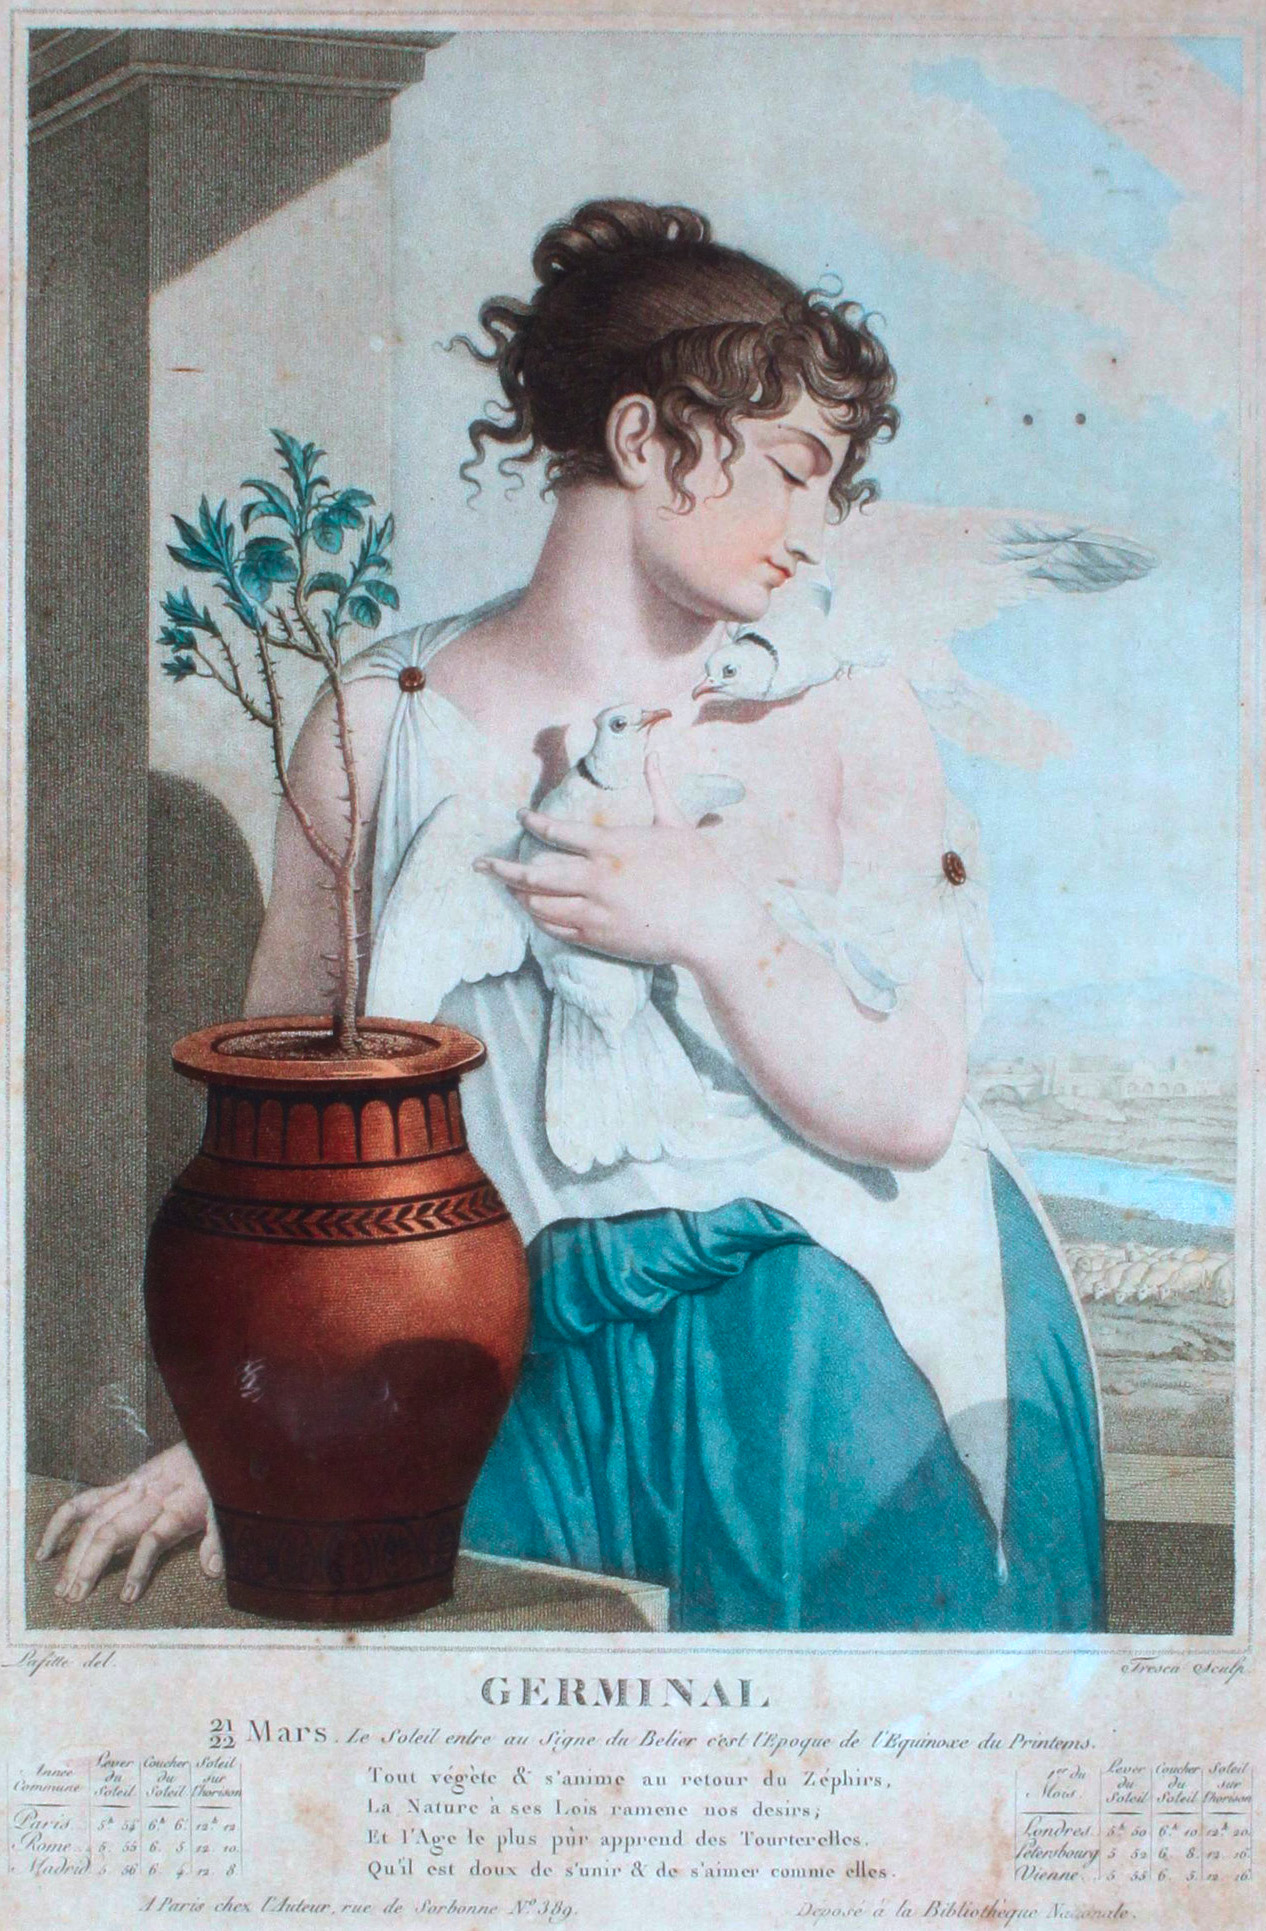
\includegraphics[width=\linewidth]{fig/germinal.jpg}
    \caption{\emph{Allégorie pour le mois de Germinal}, Louis Lafitte.}
\end{marginfigure}

A configuration of a "Turing machine"---or more generally the node of an
"automatic graph"---is said 
to be \AP""germinal"" if it has in-degree 0.%
\sidenote{A natural terminology would be ``initial'' but it clashes with the well-established notion of "initial configuration".}

\kregcolundec%

\begin{proof}%
	\proofcase{Lower bound.}
    By reduction from the "reachable regularity problem" for "linear Turing machines"
    (\Cref{lem:reachable-regularity}). We first show it for $k=2$.

    \AP Given a "linear Turing machine" $\+T$,
    observe that the set $\intro*\Germ{\+T}$ of all "germinal configurations" of $\confGraph$.
    \begin{claim}
        $\Germ{\+T}$ is effectively a "regular language". 
    \end{claim}
    
    Observe moreover that, by definition of "linear Turing machines",
    the "initial configuration" $\pad\cdot q_0 \cdot \pad$ is "germinal".
    Let $\bSymb$ and $\rSymb$ be fresh symbols. 
    Consider the "automatic graph" $\tup{V,\+E}$ for $V \defeq \configs\cdot (\bSymb + \rSymb)$,
    having an edge from $\gamma \cdot c$ to $\gamma' \cdot c$ if either 
    \begin{enumerate}
        \item $\tup{c,c'} = \tup{\bSymb,\rSymb}$ and $\gamma=\gamma'$;
        \item $\tup{c,c'} = \tup{\rSymb,\bSymb}$ and there is an edge from $\gamma$ to $\gamma'$ in $\confGraph$; or
        \item $\tup{c,c'} = \tup{\bSymb,\bSymb}$, $\gamma$ is the "initial configuration",
        and $\gamma' \neq \gamma$ is "germinal".
    \end{enumerate}

    \begin{marginfigure}%
        \centering
        \begin{tikzpicture}
            \input{tikz/dichotomy/conf-graph-wf-RTM}
        \end{tikzpicture}
        \caption{
            \AP\label{fig:reduction-wf-RTM-to-colouring-config-graph-wf-RTM}
            Configuration graph of a "linear Turing machine".
        }
    \end{marginfigure}%
    \begin{marginfigure}%
        \centering
        \begin{tikzpicture}
            \input{tikz/dichotomy/reduction-wf-RTM}
        \end{tikzpicture}
        \caption{
            \AP\label{fig:reduction-wf-RTM-to-colouring}
            The "automatic graph" to which the "configuration graph"
            of \Cref{fig:reduction-wf-RTM-to-colouring-config-graph-wf-RTM} is reduced.
        }
    \end{marginfigure}%

    Symbols $\bSymb$ and $\rSymb$ are utilized to represent two versions of each configuration.
    This graph is depicted in \Cref{fig:reduction-wf-RTM-to-colouring}.
    Note that $\tup{V,\+E}$ is "connected" and "2-colourable": in fact, it is a "directed tree" whose root is $\pad\cdot q_0\cdot \pad\cdot \bSymb$. 
    
    We claim that $\tup{V,\+E}$ is "regularly $2$-colourable" if, and only if, the set of "reachable configurations" of $T$ is a "regular language". 
    In fact, up to permuting the two-colours, $\tup{V,\+E}$
    admits a unique 2-colouring $\tup{C_1,C_2}$, defined by:
    \[
        C_1 \defeq \Reach{\+T}\cdot\bSymb \cup (\configs \setminus \Reach{\+T})\cdot\rSymb
    \]
    and $C_2$ is the complement of $C_1$.
    If $\Reach{\+T}$ is regular, then so is $C_1$. Dually, if $C_1$ is regular, then
    $\Reach{\+T}$ is exactly the set of configurations $\gamma$ such that
    $\gamma\cdot \bSymb \in C_1$ and hence is regular.
    It follows that $\tup{V,\+E}$ is "regularly $2$-colourable" if and only if
    the "reachable configurations" of $\+T$ are regular, which concludes the proof for $k=2$.

    To prove the statement for any $k>2$, we define $\tup{V,\+E_k}$ as the result of adding a $(k-2)$-clique to $\tup{V,\+E}$ and adding an edge from every vertex of the clique to every vertex incident to an edge of $\+E$. This forces the clique to use $k-2$ colours that cannot be used in the remaining part of the graph and the proof is then analogous.

	\proofcase{Upper-bound.} We show that the problem is "RE". Let us define a \AP""$k$-coloured automaton"" like a regular (complete) DFA, except that instead of having
	a set of final states, it has a partition $\langle C_1,\hdots,C_k \rangle$ of its states.
	Such an automaton recognizes a "regular colouring" $\Sigma^* \to \lBrack 1, k\rBrack$.
	Given an "automatic graph" $\+G = \tup{V,\+E}$---whose edge relations is given by
    a "synchronous automaton" $\relPres{\+E}{\+G}$---and a $k$-coloured automaton $\+B$,
	we can build, by a product construction, an automaton $\+A'$ which accepts
	all $u \otimes v \in \convolRel{R}$ such that the colour of $u$ is distinct from
    the colour of $v$.
	Then, $\+A'$ is equivalent to $\relPres{\+E}{\+G}$ if, and only if,
    $\+B$ describes a proper "$k$-colouring" of $\tup{V,\+E}$.
    The "RE" upper-bound of the "regular $k$-colourability problem" follows: 
    it suffices to enumerate all "$k$-coloured automata" and check for equivalence.
\end{proof}

Note that this reduction provides an easy way of building
graphs in the shape of \Cref{fig:reduction-wf-RTM-to-colouring} that are "2-colourable" (in fact, they are trees) but not "regularly $2$-colourable". In fact, we can provide a slightly more
direct construction.

\begin{figure}
    \centering
    \begin{tikzpicture}
        \input{tikz/dichotomy/tree-not-2reg-colour}
    \end{tikzpicture}
    \caption{
        \label{fig:tree-not-2reg-colour}
        The "automatic tree@automatic graph" $\+T$ of \Cref{ex:tree-not-2-reg-colourable},
        and its unique "$2$-colouring" $(C, V\setminus C)$, which is not "regular@@colouring".
    }
\end{figure}
\begin{example}
    \AP\label{ex:tree-not-2-reg-colourable}
    On the alphabet $\Sigma = \{a,b\}$, the tree $\+T$ depicted in \Cref{fig:tree-not-2reg-colour} whose set of vertices is $V = a^*b^*$ and whose set 
    of edges is $\+E = \+E_{\mathrm{incr}} \cup \+E_{\mathrm{init}}$, with 
    \begin{align*}
        \+E_{\mathrm{incr}} & = \{(a^pb^q,\, a^{p+1}b^{q+1}) \mid p,q \in \N\} \\
        \+E_{\mathrm{init}} & = \{(\varepsilon,\, a^p) \mid p \in \N\} \cup \{(\varepsilon,\, b^q) \mid q \in \N\}, 
    \end{align*}    
    is "automatic@automatic graph" but not "regularly $2$-colourable".
    Indeed, its only "$2$-colouring"
    consists in partitioning the vertices of $\+T$ into
    \begin{align*}
        C =\;& \{a^n b^n \mid n \in 2\N\} \\
            & \cup \{a^p b^q \mid p > q \text{ and $q$ is odd}\} \\
            & \cup \{a^p b^q \mid p < q \text{ and $p$ is odd}\}
    \end{align*}
    and its complement $V \setminus C$.
    Let $P = \{a^p b^q \mid p, q \in 2\N\} = (aa)^*(bb)^*$:
    $P$ is regular, yet $C \cap P = \{a^n b^n \mid n \in 2\N\}$ is not.
    Hence, $C$ is not regular, and thus $\+T$ is not "regularly $2$-colourable".
\end{example}
\subsection{Bounded Recognizable Relations}

\paragraph*{Separability for Bounded Recognizable Relations.}

In this section we capitalize on the undecidability result of the previous section, showing how this implies the undecidability for the "separability problem" on two natural classes of bounded "recognizable relations", namely: $\kREC$, and $\kPROD$.
Remember that, for any $k$, $\reintro*\kPROD$ is the subclass of $\REC$ consisting of unions of $k$ cross-products of regular languages (which is a subclass of $\kREC[2^{2k}]$).

First, observe that the $\kREC[1]$-"separability problem" is trivially decidable, since the only possible "separator" is $\Sigma^* \times \Sigma^*$. However, for any other $k>1$, the problem is undecidable.

\begin{proposition}
    The $\kREC$-"separability problem" is undecidable, for every $k>1$.
\end{proposition}
\begin{proof}
A consequence of the reduction from the "$k$-regular colourability problem" of \Cref{thm:reg-colourability-equiv-separability}, combined with the undecidability of the latter for every $k>1$ (\Cref{thm:k-reg-col-undec}).
\end{proof}

On the $\kPROD$ hierarchy we will find the same phenomenon. In particular the case $k=1$ is also trivially decidable.

\begin{proposition}
    The $\kPROD[1]$-"separability problem" is decidable.
\end{proposition}
\begin{proof}
    Given two "automatic relations" $R_1, R_2$, there exists $S \in $ \kPROD[1]
    that "separates" $R_1$ from $R_2$ if and only if $\pi_1(R_1)\times \pi_2(R_1)$
    "separates" $R_1$ from $R_2$.
\end{proof}

As soon as $k>1$, the $\kPROD$ "separability problem" becomes undecidable. This is a consequence of the following simple lemma.

\begin{lemma}
    A symmetric "automatic relation" $R$ and the identity $\Id$ are "separable" by a relation in $\kPROD[2]$ iff they have a "separator" of the form $(A \times B) \cup (B \times A)$.
\end{lemma}
\begin{proof}
    Assume that $S \in \kPROD[2]$ "separates" $R$ from $\Id$.
    Then $R \subseteq S$, but since $R$ is symmetric, $R = R^{-1} \subseteq S^{-1}$ so
    $R \subseteq S \cap S^{-1}$, and hence $R \subseteq S \cap S^{-1}$.
    Moreover, since $S$ has a trivial intersection with $\Id$, so does $S \cap S^{-1}$.
    Hence, $S \cap S^{-1}$ "separates" $R$ from $\Id$.

    Since $S \in \kPROD[2]$, there exists $A_1,A_2,B_1,B_2 \subseteq \Sigma^*$ such that
    $S = A_1 \times B_1 \cup B_2 \times A_2$.
    Note that $S \cap \Id = \emptyset$ yields $A_i \cap B_i = \emptyset$ for each $i \in \{1,2\}$.
    Finally:
    \begin{align*}
        S \cap S^{-1} &
        =
            \bigl( A_1 \times B_1 \cup B_2 \times A_2 \bigr)
            \cap \bigl( B_1 \times A_1 \cup A_2 \times B_2 \bigr) \\
        &
        =
            \bigl( (A_1 \times B_1) \cap (B_1 \times A_1) \bigr)
            \cup \bigl( (A_1 \times B_1) \cap (A_2 \times B_2) \bigr) \\
        &
        \hphantom{=\;} \cup \bigl( (B_2 \times A_2) \cap (B_1 \times A_1) \bigr)
            \cup \bigl( (B_2 \times A_2) \cap (A_2 \times B_2) \bigr) \\
        &
        =
            \bigl( \overbrace{(A_1 \cap B_1) \times (A_1 \cap B_1)}^{= \emptyset} \bigr)
            \cup \bigl( (A_1 \cap A_2) \times (B_1 \cap B_2) \bigr) \\
        &
        \hphantom{=\;} \cup \bigl( (B_1 \cap B_2) \times (A_1 \cap A_2) \bigr)
            \cup \bigl( \underbrace{(A_2 \cap B_2) \times (A_2 \cap B_2)}_{= \emptyset} \bigr)\\
        &
        = \bigl( (A_1 \cap A_2) \times (B_1 \cap B_2) \bigr)
            \cup \bigl( (B_1 \cap B_2) \times (A_1 \cap A_2) \bigr).\qedhere
    \end{align*}
\end{proof}

We can then establish the following: 

\begin{corollary}\AP\label{cor:2reg-2prod}
    A symmetric "automatic relation" $R$ and $\Id$ are "separable" by a relation in $\kPROD[2]$ if{f} $\AutGraph{\Sigma^*}{R}$ is "$2$-regular colourable".
\end{corollary}
\begin{proof}
    By observing that for any symmetric relation $R \subseteq \Sigma^* \times \Sigma^*$, we have that $A,B \subseteq \Sigma^*$ is a colouring of $\AutGraph{\Sigma^*}{R}$ if, and only if, $(A \times B) \cup (B \times A)$ "separates" $R$ from $\Id$.
\end{proof}

We can now easily show undecidability for the $\kPROD[2]$ "separability problem" by reduction from the "$2$-regular colourability problem".
\begin{lemma}\AP\label{lem:aut-2prod-sep-undec}
    The $\kPROD[2]$-"separability problem" is undecidable.
\end{lemma}
\begin{proof}
    By reduction from the "$2$-regular colourability problem" on "automatic graphs", which is undecidable by \Cref{thm:k-reg-col-undec}. Let $\AutGraph{L}{R}$ be an "automatic graph" and $\AutGraph{L}{R'}$ the symmetric closure of $\AutGraph{L}{R}$. It follows that $\AutGraph{L}{R'}$ is still "automatic" and that there is a "$2$-regular colouring" for $\AutGraph{L}{R'}$ if{f} there is a "$2$-regular colouring" for $\AutGraph{L}{R}$ (the same colouring in fact).
    Thus, by \Cref{cor:2reg-2prod}, $\AutGraph{L}{R}$ is "$2$-regular colourable" if{f} 
    there is a $\kPROD[2]$ relation that "separates" $R'$ from $\Id$.
\end{proof}

Further, this implies undecidability for every larger $k$:
\begin{theorem}
    \AP\label{thm:kprod-undecidable}
    The $\kPROD$-"separability problem" is undecidable, for every $k \geq 2$.
\end{theorem}

\begin{figure}
    \centering
    \begin{tikzpicture}
        \input{tikz/dichotomy/2prod-to-kprod}
    \end{tikzpicture}
    \caption{
        \AP\label{fig:2prod-to-kprod}
        Construction in the proof of \Cref{thm:kprod-undecidable} for $k = 5$. $S$ is depicted as the union of two (gray) rectangles since $S \in \kPROD[2]$.
        The relation $R'_1$ is obtained from $R_1$ (blue shape) by adding all blue edges,
        namely $(a_i, b_i)$ for $1\leq i \leq k-2$. The relation $R'_2$ is obtained from $R_2$ (red shape) by adding
        all red edges, namely every other edge involving a vertex $a_i$ or $b_i$.
        Finally, $S'$ (five gray rectangles) is obtained from $S$ by adding
        each $\{a_i\} \times \{b_i\}$.
    }
\end{figure}

\begin{proof}
    The case $k=2$ is shown in \Cref{lem:aut-2prod-sep-undec}, so suppose $k>2$.
    The proof goes by reduction from the $\kPROD[2]$-"separability problem". Let $R_1,R_2$ be a pair of "automatic relations" over an alphabet $\Sigma$. Consider the alphabet extended with $2(k-2)$ fresh symbols $\Sigma' = \Sigma \dcup \set{a_1, \dotsc, a_{k-2}, b_1, \dotsc, b_{k-2}}$. We build "automatic relations" $R'_1,R'_2$ over $\Sigma'$ such that $(R_1,R_2)$ are $\kPROD[2]$ "separable" over $\Sigma$ if{f} $(R'_1,R'_2)$ are $\kPROD$ "separable" over $\Sigma'$.

    Let $R'_1 = R_1 \dcup \set{ (a_i,b_i) : 1 \leq i \leq k-2}$ and 
    \begin{align*}
    R'_2 =  R_2 \dcup {}&\set{(a_i,w) : w \in \Sigma^*, 1 \leq i \leq k-2} \dcup {}\\
                    &\set{(w,b_i) : w \in \Sigma^*, 1 \leq i \leq k-2} \dcup {}\\
                    &\set{(a_i,b_j) : 1 \leq i,j \leq k-2, i \neq j} \dcup {}\\
                    &\set{(b_i,a_j) : 1 \leq i,j \leq k-2}
    \end{align*}
    
    If $(R_1,R_2)$ has a $\kPROD[2]$ "separator" $S$, then $\tilde S \dcup \set{(a_i,b_i) : 1 \leq i \leq k-2}$ is a $\kPROD$ "separator" of $(R'_1,R'_2)$.
    

    Conversely, if $S' = (A_1 \times B_1) \cup \dotsb \cup (A_k \times B_k)$ is a $\kPROD$ "separator" of $(R'_1,R'_2)$, then for every $i$ there must be some $j_i$ such that $A_{j_i} \times B_{j_i}$ contains $(a_i,b_i)$. Observe that 
    \begin{itemize}
        \item $A_{j_i} \cup B_{j_i}$ cannot contain any $a_{i'}$ or $b_{i'}$ for $i' \neq i$, and
        \item $A_{j_i} \cup B_{j_i}$ cannot contain any $w \in \Sigma^*$;
    \end{itemize}
    since otherwise we would have $(A_{j_i} \times B_{j_i}) \cap R'_2 \neq \emptyset$.
    Hence, $\set{i \mapsto j_i}_i$ is injective, and thus $S'$ is of the form $S' = (A_1 \times B_1) \cup (A_2 \times B_2)  \cup (\set{a_1} \times \set{b_1}) \cup \dotsb \cup (\set{a_{k-2}} \times \set{b_{k-2}})$. We can further assume that $A_1,B_1,A_2,B_2$ do not contain any $a_i$ or $b_i$ since otherwise we can remove them preserving the property of being a $\kPROD$ "separator" of $R'_1$ and $R'_2$.
    Hence, $S \defeq (A_1 \times B_1) \cup (A_2 \times B_2)$ must cover $R_1$ and be disjoint from $R_2$, obtaining that $S$ is a $\kPROD[2]$ "separator" of $R_1$ and $R_2$.
\end{proof}


\paragraph*{Definability for Bounded Recognizable Relations.}
Up until now, we have examined two hierarchies of bounded recognizable relations, namely $\kPROD$ and $\kREC$. 
Our previous analysis demonstrated that, for any element in these hierarchies (where $k>1$), the "separability problem" is undecidable. Nevertheless, 
we will now establish that the "definability problem" is decidable.

\AP Given an "automatic" relation $R \subseteq \Sigma^* \times \Sigma^*$, consider the "automatic" equivalence relation $\intro*\autequiv \subseteq \Sigma^* \times \Sigma^*$, defined as $w \mathrel{\autequiv} w'$ if for every $v \in \Sigma^*$ we have 
\begin{enumerate}
    \item $(w,v) \in R$ if{f} $(w',v) \in R$, and
    \item $(v,w) \in R$ if{f} $(v,w') \in R$.
\end{enumerate}

It turns out that equivalence classes of $\autequiv$ define the coarsest partition onto which $R$ can be recognized in terms of $\kREC$:

\begin{lemma}\AP\label{lem:krec-characterization}
    For every "automatic" $R \subseteq \Sigma^* \times \Sigma^*$, $\autequiv$ has index at most $k$ if, and only if, $R$ is in $\kREC$.
\end{lemma}
\begin{proof}
    \proofcase{Left-to-right}
    Assume that $\autequiv$ has the equivalence classes $E_1, \dotsc, E_k$. Consider the set $P \subseteq \set{1, \dotsc, k}^2$ of all pairs $(i,j)$ such that there are $u_i \in E_i$ and $u_j \in E_j$ with $(u_i,u_j) \in R$. Define the $\kREC$ relation $R' = \bigcup_{(i,j) \in P} E_i \times E_j$. We claim that $R=R'$. 
    In fact, by definition of $\autequiv$, note that if there are $u_i \in E_i$ and $u_j \in E_j$ with $(u_i,u_j) \in R$, then $E_i \times E_j \subseteq R$. Hence, $R' \subseteq R$.
    On the other hand, for every pair $(u,v) \in R$ there is $(i,j) \in P$ such that $u \in E_i$, $v \in E_j$ implying $(u,v) \in R'$.
    Hence, $R \subseteq R'$.

    \proofcase{Right-to-left}
    If $R$ is a union of products of sets from the partition $E_1 \dcup \dotsb \dcup E_k = \Sigma^*$, then every two elements of each $E_i$ are $\autequiv$-related, and thus $\autequiv$ has index at most $k$.
\end{proof}

We can then conclude that the definability problem for $\kREC$ is decidable. 

\begin{corollary}
    The $\kREC$-"definability problem" is decidable, for every $k > 0$.
\end{corollary}
\begin{proof}
    An "automatic relation" $R$ is in $\kREC$ if{f} $\autequiv$ has at most $k$ equivalence classes by \Cref{lem:krec-characterization}. 
    % This can be tested with the formula $\forall w_1, \dotsc, w_{k+1} ~ \bigvee_{i \neq j} w_i \mathrel{\autequiv} w_j$.
    %    
    In other words, an "automatic relation" $R$ is not in $\kREC$ if{f} the complement of $\autequiv$ contains a $(k+1)$-clique, which can be easily tested.
\end{proof}

The relation $\autequiv$ can also be used to characterize which automatic relations are definable in the class $\kPROD$.

\begin{lemma}
    An "automatic relation" $R$ is in $\kPROD$ if, and only if, $R=(A_1 \times B_1) \cup \dotsb \cup (A_k \times B_k)$ where each $A_i$ and $B_i$ is a union of equivalence classes of $\autequiv$.
\end{lemma}
\begin{proof}
    It suffices to show that for every equivalence class $E$ from $\autequiv$, if $A_1 \cap E \neq \emptyset$ then $R = ((A_1 \cup E) \times B_1) \cup \dotsb \cup (A_k \times B_k)$, and similarly for $B_1$. Assume $w \in A_1 \cap E$ and take any pair $(u,v) \in E \times B_1$. We show that $(u,v) \in R$. By definition of $\autequiv$, since $(w,v) \in R$ and $w \mathrel{\autequiv} u$, we have that $(u,v) \in R$.
\end{proof}

Again, this characterization allows us to show that definability in the class $\kPROD$ is decidable. 

\begin{corollary}
    The $\kPROD$-"definability problem" is decidable, for every $k > 0$.
\end{corollary}

\begin{proof}
    By brute force testing whether the "automatic relation" $R$ is equivalent to $(A_1 \times B_1) \cup \dotsb \cup (A_k \times B_k)$ for every possible $A_i,B_i$ which is a union of equivalence classes of $\autequiv$.
\end{proof}

\section{Undecidability of the Homomorphism Problems}
\label{sec:dichotomy-undecidability}

\subsection{Overview \& Easy Implications of the Dichotomy Theorem}
\label{sec:dichotomy-overview}

\begin{mainstatement}
	\DichotomyThmDichotomyAutomatic
\end{mainstatement}

\begin{remark}
	\todo{TODO GEneralization to "higher-order automatic structures".}
	\todo{Deterministic rational?}
	\todo{RHS is "automatic@@struct"?}
\end{remark}

\begin{marginfigure}
	\centering
	\begin{tikzpicture}
		\node (1) at (0,0) {\itemDTFinDual};
\node[below=2em of 1] (5) {\itemDTFirstOrder};
\node[below=2em of 5] (4) {\itemDTEqual};
\node[below left=2em and -1em of 4] (3) {\itemDTHomRegDec};
\node[below right=2em and -1em of 4] (2) {\itemDTHomDec};

% ---
% Transitions
% ---
\draw[implication] (1) to (5);
\draw[implication] (5) to (4);
\draw[implication] (4) to (3);
\draw[implication] (4) to (2);
\draw[implication, bend left=30] (3) to (1.west);
\draw[implication, bend right=30] (2) to (1.east);
	\end{tikzpicture}
	\caption{\AP\label{fig:dichotomy-overview}Implications shown in the chapter to prove
	\Cref{thm:dichotomy-theorem-automatic-structures}.}
\end{marginfigure}
We prove \Cref{thm:dichotomy-theorem-automatic-structures} by showing the
implications depicted in \Cref{fig:dichotomy-overview}.
The most difficult implications are $\itemDTFinDual \Rightarrow \itemDTFirstOrder$,
which we prove in \Cref{sec:dichotomy-decidability}, and the implications
$\itemDTHomDec \Rightarrow \itemDTFinDual$ and $\itemDTHomRegDec \Rightarrow \itemDTFinDual$,
which we prove by contraposition in \Cref{sec:undecidability-hom,sec:undecidability-homreg}.

On the other hand, the implications $\itemDTFirstOrder \Rightarrow \itemDTEqual$,
$\itemDTEqual \Rightarrow \itemDTHomRegDec$ and $\itemDTEqual \Rightarrow \itemDTHomDec$ are straightforward: we prove them in this section. 
Before showing these implications, we start by proving $\itemDTFinDual \Rightarrow \itemDTHomDec$.\footnote{While it is redundant with the implications of \Cref{fig:dichotomy-overview}, 
we prove this implication for two reasons: not only is it straightforward, it is also
the implication which, together with the fact that both $\HomAut{\clique{2}}$
and $\HomRegAut{\clique{2}}$ are undecidable by
\cite[Proposition 6.5]{Kocher2014AutomatischenGraphen}
and \cite[Theorem 4.4]{BarceloFigueiraMorvan2023SeparatingAutomatic}, that lead us to conjecture
\Cref{thm:dichotomy-theorem-automatic-structures}.}

\paragraph*{Decidability of the Homomorphism Problem.}

\begin{proposition}
	\!\footnote{This corresponds to the implication $\itemDTFinDual \Rightarrow \itemDTHomDec$
	of \Cref{thm:dichotomy-theorem-automatic-structures}.}
	\AP\label{prop:dichotomy-FinDual-implies-HomDec}
	Let $\?B$ be a "finite $\sigma$-structure".
	If $\?B$ has finite duality, then $\HomAut{\?B}$ is decidable in "NL".
\end{proposition}

\begin{proof}
	Given a "finite $\sigma$-structure" $\?D$ with domain $\{d_1,\hdots,d_n\}$,
	we build the "first-order sentence"
	\[
		\phi_{\?D} \defeq \exists x_1.\; \cdots \exists x_n.\;
		\bigwedge_{\+R_{(k)} \in \sigma} \bigwedge_{\substack{\tup{i_1,\hdots,i_k} \in \lBrack 1,n\rBrack^k\\\text{"st" }\tup{d_{i_1},\hdots,d_{i_k}} \in \+R(\?D)}}
		\+R(x_{i_1},\hdots,x_{i_k}).
	\]
	By construction, for any arbitrary "$\sigma$-structure" $\?A$, we have $\?A \FOmodels \phi_{\?D}$
	"iff" $\?D \homto \?A$.
	Then, since $\?B$ has "finite duality", it admits a finite "dual"
	$\?D_1,\hdots,\?D_m$.
	Then
	\[
		\?A \FOmodels \bigwedge_{i=1}^m \neg \phi_{\?D_i}
		\quad\text{"iff"}\quad 
		\?A \homto \?B.
	\]
	The conclusion follows from the fact that the "data complexity"
	of "first-order model checking of automatic structures" is "NL"
	by \Cref{prop:first-order-model-checking-automatic-structures}.
\end{proof}

Note that \Cref{prop:dichotomy-FinDual-implies-HomDec} still holds
when the "homomorphism problem" takes as input "higher-order automatic
structures" since such structures have a decidable first-order theory.


\paragraph*{Uniformly First-Order Definable Homomorphisms Imply Equality.}

\begin{proposition}
	\!\footnote{This corresponds to the implication $\itemDTFirstOrder \Rightarrow \itemDTEqual$
	of \Cref{thm:dichotomy-theorem-automatic-structures}.}
	\AP\label{prop:dichotomy-FirstOrder-implies-Equal}.
	Let $\?B$ be a "finite $\sigma$-structure".
	If $\HomAll{\?B}$ has "uniformly first-order definable homomorphisms", then
	$\HomAut{\?B} = \HomRegAut{\?B}$.
\end{proposition}

\begin{proof}
	By assumption,there exists "first-order formulas"
	$\langle \phi_b(x) \rangle_{b\in B}$ over $\sigma$ "st" for any
	arbitrary "$\sigma$-structure" $\?A$, for any $a\in A$,
	there is at most one $b \in B$ "st" $\langle \?A, a \rangle \FOmodels \phi_b(x)$, and moreover $\?A \homto \?B$
	"iff" for each $a\in A$, there is exactly one $b(a) \in B$ "st" $\langle \?A, a \rangle \FOmodels \phi_{b(a)}(x)$, and $a \mapsto b(a)$ is a "homomorphism".
	Now, when the right-hand side holds, given an "automatic structure" $\+A$,
	for each $b\in \?B$, we let $\tilde\phi_b(x)$ be the "first-order formula" over $\signatureSynchronous{\Sigma}$ obtained from $\phi_b(x)$
	by substituting $\+R(x_1,\hdots,x_k)$ for the "first-order formula"
	over $\signatureSynchronous{\Sigma}$ describing $\+R_{(k)}$ in $\+A$.
	It follows that if $\?A \homto \?B$, then the function
	mapping $u \in \Sigma^*$ to the unique $b \in B$ "st" $\Sigma^*, u \FOmodels \tilde\phi_b(x)$
	defines a "regular homomorphism" from $\+A$ to $\?B$---the regularity follows from
	todo:addref-first-order-iff-automatic.
	And hence $\HomAut{\?B} \subseteq \HomRegAut{\?B}$. The conclusion follows since
	the other implication is trivial.
\end{proof}

\paragraph*{Equality of the Homomorphism Problems Imply their Decidability.}

\begin{proposition}
	\!\footnote{This corresponds to the implication $\itemDTEqual \Rightarrow \itemDTHomDec$
	of \Cref{thm:dichotomy-theorem-automatic-structures}.}
	\AP\label{prop:dichotomy-Equal-implies-HomDec}.
	Let $\?B$ be a "finite $\sigma$-structure".
	If $\HomAut{\?B} = \HomRegAut{\?B}$ then $\HomAut{\?B}$ and $\HomRegAut{\?B}$
	are decidable.
\end{proposition}

To prove this, we first give an upper bound on the homomorphism problems independently
of any assumption on $\?B$.
\begin{proposition}
	\AP\label{prop:dichotomy-general-upper-bounds}
	Let $\?B$ be a "finite $\sigma$-structure".
	Then $\HomAut{\?B}$ is "coRE" and $\HomRegAut{\?B}$ is "RE".
\end{proposition}

\begin{proof}
	\proofcase{$\HomAut{\?B}$ is "coRE".}
	By the "De Bruijn–Erdős Theorem", for any arbitrary "$\sigma$-structure" $\?A$,
	we have $\?A \nothomto \?B$ "iff" there exists a finite "substructure" $\?A'$ of $\?A$
	"st" $\?A' \nothomto \?B$.
	Given a "finite $\sigma$-structure" $\?A'$ and an "automatic $\sigma$-structure",
	it is decidable whether $\?A'$ is a "substructure" of $\?A$: indeed, it suffices
	to check, using \Cref{prop:first-order-model-checking-automatic-structures} if
	\[
		\Bigl(
			\exists x_1,\; \cdots \exists x_n,\;
			\bigwedge_{\+R_{(k)} \in \sigma} \bigwedge_{\substack{\tup{i_1,\hdots,i_k} \in \lBrack 1,n\rBrack^k\\\text{"st" }\tup{a_{i_1},\hdots,a_{i_k}} \in \+R(\?A')}}
			\+R(x_{i_1},\hdots,x_{i_k})
		\Bigr)
		\FOmodels^{?} \?A,
	\]
	by letting $\{a_1,\hdots,a_n\} = A'$. 
	Moreover, whether $\?A' \nothomto \?B$ is also decidable---in "coNP"---by \todo{addref}.
	Overall, this provides a co-semi-algorithm for $\HomAut{\?B}$: we enumerate finite
	"$\sigma$-structure" $\?A'$, and test if (1) $\?A'$ is a "substructure" of $\?A$ and if (2)
	$\?A' \homto \?B$. And hence $\HomAut{\?B}$ is "coRE".

	\proofcase{$\HomRegAut{\?B}$ is "RE".} This is an easy generalization of
	\Cref{thm:k-reg-col-undec}: instead of having "$k$-coloured automaton", we define
	``$\?B$-automaton'', that admit a partition $\langle C_{b} \rangle_{b \in B}$.
	The semantics of such an automaton is a partial function $f\colon \Sigma^* \to B$. 
	Given an "automatic structure" $\+A$, we can then effectively test if $f$ is defined on $\domainPres{\+A}$, and if $f$ defines a "homomorphism" from $\?A$ to $\?B$---see
	the proof of \Cref{thm:k-reg-col-undec}. If so, $\+A \homregto \?B$. Dually, any "regular homomorphism" $\+A \homregto \?B$ can be described by such a $\?B$-automaton.
	Therefore, $\HomRegAut{\?B}$ is "RE".
\end{proof}

\begin{proof}[Proof of \Cref{prop:dichotomy-Equal-implies-HomDec}.]
	If $\HomAut{\?B} = \HomRegAut{\?B}$, then by \Cref{prop:dichotomy-general-upper-bounds},
	these problems are both "RE" and "coRE", and are hence decidable.
\end{proof}

\subsection{Undecidability of \,$\HomAut{\?B}$}
\label{sec:undecidability-hom}

We now prove the undecidability of $\HomAut{\?B}$ and $\HomRegAut{\?B}$
when $\?B$ does not have "finite duality". Both reductions are
direct adaptations of the proof that $\HomFin{\?B}$ is "L"-hard when $\?B$ does not
have finite duality by \textcite[Theorem 3.2]{LaroseTesson2009UniversalAlgebraCSP}.
However, proving the undecidability of the problem that is reduced
to $\HomRegAut{\?B}$ is not entirely trivial and requires some work.
\begin{itemize}
	\item For $\HomFin{\?B}$, we reduce the complement of "Connectivity in automatic graphs",
		providing a "coRE"-lowerbound.
	\item For $\HomRegAut{\?B}$, we reduce "regular unconnectivity in automatic graphs",
		which in turn is reduced from \todo{update}.
\end{itemize}

For $n\in\N$, we define the \AP""$n$-link"" $\intro*\link{n}$ be the "$\sigma$-structure"\sidenote{From \cite[\S~2]{LaroseLotenTardif2007CharacterisationFOCSP}.} 
whose domain is $\lBrack 0,n\rBrack$, and every "predicate" $\+R$
of arity $k$, is interpreted as the set of tuples $\langle a_1,\, \hdots,\, a_k \rangle$
"st" $|a_i-a_j| \leq 1$ for all $i,j \in \lBrack 0,n \rBrack$. See \Cref{fig:n-link}.
\begin{marginfigure}
	\centering
	\begin{tikzpicture}
		\node[vertex] (0) at (0,0) {};
\node[vertex, right=of 0] (1) {};
\node[vertex, right=of 1] (2) {};
\node[vertex, right=of 2, opacity=0] (3) {};
\node[vertex, right=of 3] (4) {};
\node[yshift=-.1em] at (3) (3-label)  {$\cdots$};

% ---
% Transitions
% ---
\foreach \i in {0,1,2,3} {
	\pgfmathtruncatemacro{\next}{\i + 1}
	\draw[edge, bend right=30] (\i) to (\next);
	\draw[edge, bend right=30] (\next) to (\i);
};
\foreach \i in {0,1,2,4} {
	\draw[edge, loop, out=60,in=120,looseness=6] (\i) to (\i);
}
	\end{tikzpicture}
	\caption{\AP\label{fig:n-link}The "$n$-link" $\link{n}$ over the "graph signature".}
\end{marginfigure}
Given a "$\sigma$-structure" $\?B$, say that $b \in \?B$ and $b'$ are
\AP""$n$-linked"" if there exists a "homomorphism" from $\link{n}$ to $\?B$
that sends $0$ to $b$ and $n$ to $b'$. We say that $b$ and $b'$ are \AP\reintro{linked} if
they are "$n$-linked" for some $n \in \N$.

Note that the fact that $k \mapsto n-k$
defines an "automorphism" of $\link{n}$ implies that the relation of being "$n$-linked"---%
and to a greater extent of being "linked"---is symmetric.
Moreover, being "linked" is transitive, but not necessarily reflexive.

% \begin{fact}[Link Composition]
% 	\AP\label{fact:link-composition}
% 	Let $n,m \in \N$, let $\?B$ be a "$\sigma$-structure", and let $b,b',b'' \in B$.
% 	If $b$ and $b'$ are "$n$-linked" and $b'$ and $b''$ are "$m$-linked", then
% 	$b$ and $b''$ are "$(n+m)$-linked".
% \end{fact}
% We define the binary relation $\sim_n$
% on $\link{n} \prodstruct \iterstruct{\?B}{2}$ as follows:\sidenote{From \cite[\S~4.3]{LaroseLotenTardif2007CharacterisationFOCSP}.}%
% \[
% 	\langle k,\, b_1,\, b_2\rangle \sim_n \langle k',\, b'_1,\, b'_2\rangle
% 	\quad\text{when}\quad
% 	\begin{cases*}
% 		\;\langle k,\,  b_1,\, b_2\rangle = \langle k',\, b'_1,\, b'_2\rangle\text{, or}\\
% 		\;k = k' = 0 \text{ and } b_1 = b'_1\text{, or}\\
% 		\;k = k' = n \text{ and } b_2 = b'_2.
% 	\end{cases*}
% \]

\begin{proposition}[{\cite[Theorem 4.7]{LaroseLotenTardif2007CharacterisationFOCSP}}]%
	\!\footnote{Actually \cite[Theorem 4.7]{LaroseLotenTardif2007CharacterisationFOCSP} assumes
	that $\HomFin{\?B}$ is "first-order definable", but this condition
	is equivalent to $\?B$ having "finite duality" by Atserias' result
	\cite[Corollary 4]{Atserias2008DigraphColoring}.}%
	%%%
	\AP\label{prop:characterization-finite-duality-path-projections}
	An arbitrary "$\sigma$-structure" $\?B$ has "finite duality" "iff"
	$\projHom{1}$ and $\projHom{2}$ are "linked" in $\powstruct{\?B}{(\iterstruct{\?B}{2})}$.
\end{proposition}

Equipped with the previous proposition, we can now show the undecidability 
of $\HomAut{\?B}$ by reduction from the following problem.

\decisionproblem{""Connectivity in Automatic Graphs""}{
	A "automatic presentation of a directed graph" $\•G$,
	and two elements $s,t \in \Sigma^*$.
}{
	Are $\•G(s)$ and $\•G(t)$ "connected" in $\?G$?
}
\begin{property}
	\AP\label{prop:undecidability-connectivity}
	For any "signature" $\sigma$ containing at least one "predicate" of
	arity at least 2, "Connectivity in automatic graphs" is "RE"-complete.
\end{property}

\begin{proof}
	This follows from the fact that the "configuration graph" of
	a "Turing machine" is always "automatic@@struct" by \todo{addref}.
	\todo{Give more precisions.}
\end{proof}

\begin{lemma}
	\AP\label{lem:reduction-hom}
	Assume that $\sigma$ contains at least one "predicate" of arity at least 2.
	If $\?B$ does not have "finite duality", then there is a "first-order reduction" 
	from the complement of "connectivity in automatic graphs" to $\HomAut{\marked{\?B}}$.
\end{lemma}

\begin{marginfigure}
	\centering
	\begin{tikzpicture}
		\node[vertex] (0) at (0,0) {};
\node[vertex, right = 2.5 em of 0] (1) {};
\node[vertex, above right = 1em and 2em of 1] (2) {};
\node[vertex, below right = 1em and 2em of 1] (3) {};

\draw[edge] (1) to (2);
\draw[edge, bend right=15] (2) to (3);
\draw[edge, bend right=15] (3) to (2);
\draw[edge] (1) to (3);
	\end{tikzpicture}
	\caption{
		\AP\label{fig:graph-to-struct-graph}
		A "graph@@dir" $\?G$.
	}
\end{marginfigure}
\begin{marginfigure}
	\centering
	\begin{tikzpicture}
		\node[vertex] (0) at (0,0) {};
\node[vertex, right = 2.5 em of 0] (1) {};
\node[vertex, above right = 1em and 2em of 1] (2) {};
\node[vertex, below right = 1em and 2em of 1] (3) {};

\draw[edge, bend right=15] (1) to (2);
\draw[edge, bend right=15] (2) to (1);
\draw[edge, bend right=15] (2) to (3);
\draw[edge, bend right=15] (3) to (2);
\draw[edge, bend right=15] (1) to (3);
\draw[edge, bend right=15] (3) to (1);

\draw[edge, loop, out=150,in=210,looseness=6] (1) to (1);
\draw[edge, loop, out=60,in=120,looseness=6] (2) to (2);
\draw[edge, loop, out=-120,in=-60,looseness=6] (3) to (3);
	\end{tikzpicture}
	\caption{
		\AP\label{fig:graph-to-struct-struct}
		The "structure" $\?A$ defined from $\?G$ (in \Cref{fig:graph-to-struct-graph}),
		using the construction done in the proof of \Cref{lem:reduction-hom},
		when $\sigma$ consists of a single binary relation.
	}
\end{marginfigure}

\begin{proof}
	Given an instance $\langle \•G, s, t \rangle$ of "connectivity in automatic graphs",
	we first define the $\sigma$-structure $\?A$ with "automatic presentation" $\•A$
	obtained by replacing every edge of $\•G$ by a "$1$-link".
	Formally, $\?A$ has the same domain as $\?G$, and for any
	"predicate" $\+R \in \sigma$ of arity $k$,
	$\langle g_1,\, \hdots,\, g_k \rangle \in \+R(\?A)$ "iff"
	$\{g_1, \hdots, g_k\} = \{g,g'\}$ for some $g,g' \in G$ "st"
	there is an edge from $g$ to $g'$ in $\?G$.
	See \Cref{fig:graph-to-struct-graph,fig:graph-to-struct-struct}.

	\begin{claim}
		\AP\label{claim:reduction-hom-from-graph-to-link}
		$\•G(s)$ and $\•G(t)$ are "connected" "iff"
		$\•A(s)$ and $\•A(t)$ are "linked".
	\end{claim}
	For the left-to-right implication: if there is an edge between two elements
	in $\?G$, then they are "$1$-linked" in $\?A$. Since being "linked" is
	reflexive and transitive, the conclusion follows.
	Conversely, if two elements $a$ and $a'$ of $\?A$ are "$1$-linked", 
	then pick a "predicate" $\+R \in \sigma$ of arity at least 2.
	Then $\langle a,\, \hdots,\, a,\, a' \rangle \in \+R(\?A)$,
	and so by definition of $\?A$ there is either an edge from $a$ to $a'$
	or from $a'$ to $a$ in $\?G$.\sidenote{Note that the proof of this claim
	is the only part of the proof of \Cref{lem:reduction-hom} that requires
	the assumption that $\sigma$ contains at least one "predicate" of arity at least 2.}

	We then consider the "automatic $\sigma$-structure" $\?A\prodstruct \iterstruct{\?B}{2}$,%
	\footnote{See \Cref{sec:construction-automatic-presentations} to have an explicit construction 
	of an "automatic presentation" for this structure.}
	and extend it to a
	"$\extendedSignature{\sigma}{\?B}$-structure" \AP\(\intro*\ConstrUndecHom{(\?A\prodstruct \iterstruct{\?B}{2})}\)
	in which for each $b_0 \in B$,
	we "interpret@@predicate" the unary "predicate" $\unarypred{b_0}$ as
	\[
		\big\{\;
			\langle a,\, b,\, b'\rangle \;\big\vert\;
			a = \•A(s) \text{ and } b = b_0 \text{, or }
			a = \•A(t) \text{ and } b' = b_0
		\;\big\}.
	\]
	To construct an "automatic presentation" for this structure, see \Cref{sec:construction-automatic-presentations}.
	\begin{claim}
		\AP\label{claim:reduction-hom-direct}
		If $\ConstrUndecHom{(\?A\prodstruct \iterstruct{\?B}{2})} \homto \marked{\?B}$,
		then $\•G(s)$ and $\•G(t)$ are not "connected" in $\?G$.
	\end{claim}
	Let $f\colon \ConstrUndecHom{(\?A\prodstruct \iterstruct{\?B}{2})} \homto \marked{\?B}$
	be a "homomorphism".\sidenote{Recall that both sides are
	"$\extendedSignature{\sigma}{\?B}$-structures".}
	It induces a "homomorphism"
	\[
		\overbar f\colon \?A\prodstruct \iterstruct{\?B}{2} \homto \?B
	\]
	between "$\sigma$-structures", and by currying (\Cref{prop:currying-hom}),
	$\overbar f$ can be seen as a "homomorphism"
	\[
		F\colon \?A \homto \powstruct{\?B}{(\iterstruct{\?B}{2})}.
	\]
	Note moreover that because $\overbar f$ comes from a "homomorphism" between
	$\extendedSignature{\sigma}{\?B}$ then we must have  
	$f(\•A(s),\, b,\, b') = b$
	and $f(\•A(t),\, b,\, b') = b'$ for all $b,b' \in B$.
	This implies that $F(\•A(s)) = \projHom{1}$ and $F(\•A(t)) = \projHom{2}$.
	
	We now assume by contradiction that there is some $n \in \N$
	"st" there is a "homomorphism" $g\colon \link{n} \to \?A$
	with $g(0) = \•A(s)$ and $g(n) = \•A(t)$.
	Then by composition, we obtain a "homomorphism"
	\[
		F \circ g\colon
		\link{n} \to \powstruct{\?B}{(\iterstruct{\?B}{2})},
 	\]	
	which sends $0$ to $F(g(0)) = F(\•A(s)) = \projHom{1}$
	and sends $n$ to $F(g(n)) = F(\•A(t)) = \projHom{2}$.
	So, by \Cref{prop:characterization-finite-duality-path-projections},
	$\?B$ would have "finite duality", which is a contradiction.
	Hence, $\•A(s)$ and $\•A(t)$ are not "linked",
	and so by \Cref{claim:reduction-hom-from-graph-to-link}, $\•G(s)$ and $\•G(t)$
	are not "connected".

	\begin{claim}
		\AP\label{claim:reduction-hom-converse}
		If $\•G(s)$ and $\•G(t)$ are not "connected" in $\?G$,
		then there is a "homomorphism" from
		$\ConstrUndecHom{(\?A\prodstruct \iterstruct{\?B}{2})}$ to $\marked{\?B}$.
	\end{claim}
	We define a "homomorphism" $f\colon \ConstrUndecHom{(\?A\prodstruct \iterstruct{\?B}{2})} \to \marked{\?B}$ by:
	\[
		f(a, b, b') \defeq \begin{cases*}
			\;b & \text{ if $\•A(s)$ and $a$ are "linked",} \\
			\;b' & \text{ otherwise.}
		\end{cases*}
	\]
	We show that this is indeed a "homomorphism": for any "predicate" $\+R$
	of arity $k$ in $\sigma$, if
	\[
		\langle a_1,\, b_1,\, b'_1 \rangle,\;
		\langle a_2,\, b_2,\, b'_2 \rangle,\;
		\hdots,\;
		\langle a_k,\, b_k,\, b'_k \rangle
	\]
	are all "$\+R$-hyperedges" of $\ConstrUndecHom{(\?A\prodstruct \iterstruct{\?B}{2})}$,
	then by definition of $\?A$, we have that either (1) all $a_i$'s are equal,
	or (2) $\{a_1,\, \hdots,\, a_k\} = {a,a'}$ for some $a \neq a' \in A$
	and there is an edge from $a$ to $a'$ or from $a'$ to $a$ in $\?G$.
	In both cases, it follows that $\•A(s)$ and $a_i$ are "linked"
	"iff" $\•A(s)$ and $a_j$ for all $i,j\in \lBrack 1,k\rBrack$.
	Hence, either $f(a_i,\, b_i,\, b'_i) = b_i$ for all $i\in \lBrack 1,k\rBrack$,
	or $f(a_i,\, b_i,\, b'_i) = b'_i$ for all $i\in \lBrack 1,k\rBrack$.
	In both cases, we get that
	\[
		\Big\langle
			f(a_1,\, b_1,\, b'_1),\;
			f(a_2,\, b_2,\, b'_2),\;
			\hdots,\;
			f(a_k,\, b_k,\, b'_k)
		\Big\rangle
		\in \+R(\?B).
	\]
	We also need to show that this map preserves the new unary "predicates" of
	$\extendedSignature{\sigma}{\?B}$: this follows from---and is in fact equivalent to---the
	fact that $\•A(s)$ and $\•A(t)$ are not "linked" by \Cref{claim:reduction-hom-from-graph-to-link}.
	Overall, this proves that $\ConstrUndecHom{(\?A\prodstruct \iterstruct{\?B}{2})} \homto \marked{\?B}$.

	Putting \Cref{claim:reduction-hom-direct,claim:reduction-hom-converse} together,
	we get that the reduction is correct.
	Lastly, note that it is a "first-order reduction" because \todo{TODO}.
\end{proof}

By \Cref{prop:undecidability-connectivity}, the complement of "Connectivity in automatic graphs"
is "coRE"-complete, and assuming that $\sigma$ contains at least one "predicate" of arity 2,
it reduces by \Cref{lem:reduction-hom} to any problem $\HomAut{\marked{\?B}}$ when $\?B$ has "finite duality". In turns, by \Cref{prop:idempotent-core-preserves-csp-complexity}, it reduces to
$\HomAut{\?B}$, which is thus "coRE"-hard. It remains to deal with "signatures" consisting of only
unary "predicates".\sidenote{It is not clear to us whether this case was properly handled in
\cite{LaroseLotenTardif2007CharacterisationFOCSP}.}

\begin{property}
	\AP\label{prop:finite-duality-unary-predicates}
	If $\sigma$ only consists of unary "predicates", then all "$\sigma$-structures"
	have "finite duality".
\end{property}	

\begin{proof}
	Fix a $\sigma$-structure $\?B$. We define the \AP""unary type""
	$\intro*\unaryType{b}{\?B}$ of $b \in \?B$
	to be the set of "predicates" $\+P$ "st" $b \in \+P(\?B)$.
	
	Given $\tau \subseteq \sigma$, define \AP$\intro*\structOfUnaryType{\tau}$
	to be the "$\sigma$-structure"
	consisting of a single element $*$, and "st" $* \in \+P(\?1_\tau)$ "iff"
	$\+P \in \tau$.
	We say that $\tau$ is \AP""obstructing@@unarytype"" if
	$\tau \not\subseteq \unaryType{b}{\?B}$ for all $b \in \?B$.

	\begin{claim}
		\AP\label{claim:finite-duality-unary-predicates-direct}
		If $\tau$ is "obstructing@@unarytype",
		then $\structOfUnaryType{\tau} \nothomto \?B$.
	\end{claim}
	We prove the result by contraposition.
	Any "homomorphism" from $\structOfUnaryType{\tau}$ to $\?B$
	should send $*$ on some element $b$ of $\?B$
	"st" $b \in \+P(\?B)$ for all $\+P \in \tau$, and
	hence $\tau \subseteq \unaryType{b}{\?B}$.

	\begin{claim}
		\AP\label{claim:finite-duality-unary-predicates-converse}
		If $\?A \nothomto \?B$ then there exists an "obstructing@@unarytype"
		$\tau \subseteq \sigma$ "st" $\structOfUnaryType{\tau} \homto \?A$.
	\end{claim}
	We define a partial homomorphism $f$ from $A$ to $B$,
	by sending $a \in A$ to any $b \in B$ "st" the "unary type" of $a$
	is included in the "unary type" of $b$. This is clearly a (partial) "homomorphism",
	and so since $\?A \nothomto \?B$, it follows that it must be partial,
	"ie" that some element $a \in \?A$ "st" $\unaryType{a}{\?A} \not\subseteq
	\unaryType{b}{\?B}$ for any $b \in B$. It follows that $\unaryType{a}{\?A}$
	is "obstructing@@unarytype". Since $\structOfUnaryType{\unaryType{a}{\?A}} \homto \?A$
	"via" $* \mapsto a$, the conclusion follows.

	Putting \Cref{claim:finite-duality-unary-predicates-direct,claim:finite-duality-unary-predicates-converse} together, we get that
	\[
		\big\{\;
			\structOfUnaryType{\tau}
			\;\big\vert\;
			\text{ $\tau \subseteq \sigma$ is "obstructing@@unarytype"} 
		\;\big\}
	\]
	is a finite "dual" for $\?B$.
\end{proof}

\begin{corollary}
	\!\sidenote[][-15em]{In the case of Larose and Tesson, they study the problem
	$\HomFin{-}$, and prove in \cite[Theorem 3.2]{LaroseTesson2009UniversalAlgebraCSP}
	that there is a "first-order reduction" from "Connectivity in Finite Graphs" to
	$\HomFin{\marked{\?B}}$ assuming that $\?B$ does not have finite duality.
	Moreover, "Connectivity in Finite Graphs" is "L"-hard under "first-order reductions" since
	Etessami \cite[Theorem 3.2]{Etessami1997CountingLogSpace} proved that the problem
	of given a directed path and two vertices $s$, $t$ to decide if there is a path from
	$s$ to $t$ is "L"-hard under "first-order reductions"-in fact even under quantifier-free reductions. It turn, this problem can be reduced in "first-order@@reduction"
	to "Connectivity in Finite Graphs" \cite{SamiD2015USTCONNLogspace}.
	Overall, and together with \Cref{prop:idempotent-core-preserves-csp-complexity},
	this shows that $\HomFin{\?B}$ is "L"-hard under "first-order reductions".}%
	%%%
	\AP\label{coro:lowerbound-hom}
	If $\?B$ does not have "finite duality", then $\HomAut{\?B}$
	is "coRE"-hard.
\end{corollary}

\begin{proof}
	By \Cref{prop:finite-duality-unary-predicates}, since $\?B$ does not have "finite duality",
	then $\sigma$ has at least one "predicate" of arity at least 2.
	The conclusion follows from \Cref{prop:idempotent-core-preserves-csp-complexity,prop:undecidability-connectivity,lem:reduction-hom}.
\end{proof}

\subsection{Undecidability of \,$\HomRegAut{\?B}$}
\label{sec:undecidability-homreg}

The reduction to show undecidability of is nearly identical to \Cref{lem:reduction-hom},
but the input problem differs quite a lot.
\decisionproblem{""Regular Unconnectivity in Automatic Graphs""}{
	An "automatic presentation" $\•G$ of a "directed graph" $\?G$,
	and two elements $s,t \in \Sigma^*$.
}{
	Is there a regular language $L \subseteq \Sigma^*$ 
	such that $s \in L$, $t\not\in L$ and $L$ is a union of "connected components"
	of $\•G$?\footnotemark{}
	In this case we say that $s$ and $t$ are \AP""regularly unconnected"".
}
\footnotetext{Formally, we mean that $L = \•G^{-1}[U]$ for some union $U$ of "connected components" of $\?G$.}

We will first reduce this problem to $\HomRegAut{\?B}$,
and will later settle its complexity.

\begin{lemma}
	\AP\label{lem:reduction-hom-reg}
	Assume that $\sigma$ contains at least one "predicate" of arity at least 2.
	If $\?B$ does not have "finite duality", then there is a "first-order reduction"
	from "regular unconnectivity in automatic graphs"
	to $\HomRegAut{\marked{\?B}}$.
\end{lemma}

\begin{proof}
	Given an instance $\langle \•G, s, t \rangle$ of "regular unconnectivity in automatic graphs",
	we first define the $\sigma$-structure $\?A$ with "automatic presentation" $\•A$
	obtained by replacing every edge by a "$1$-link", as in \Cref{lem:reduction-hom}.

	\begin{claim}
		\!\footnote{While ``being "linked"'' is not reflexive in general, it is over the
		structure $\?A$, by reflexivity of ``being "connected"'' in $\•G$.}%
		\AP\label{claim:reduction-homreg-from-graph-to-link}
		$\•G(s)$ and $\•G(t)$ are "regularly unconnected" "iff"
		there is no $L \subseteq \Sigma^*$ "st" $\•A(s)\in L$ and $t \not\in L$,
		and $L$ is a union of equivalences classes of $\domainPres{\•A}$
		under ``being "linked"''.
	\end{claim}
	The proof is similar to \Cref{claim:reduction-homreg-from-graph-to-link}.
	Then again, we reduce the instance $\langle \•G, s, t \rangle$
	to an "automatic presentation" of \(\ConstrUndecHom{(\?A\prodstruct \iterstruct{\?B}{2})}\),
	as in \Cref{lem:reduction-hom}.
	\begin{claim}
		\AP\label{claim:reduction-homreg-direct}
		If $\ConstrUndecHom{(\•A\prodpres \iterstruct{\?B}{2})} \homregto \marked{\?B}$,
		then $\•G(s)$ and $\•G(t)$ are "regularly unconnected" in $\?G$.
	\end{claim}
	
	Let \(f\colon \ConstrUndecHom{(\•A\prodpres \iterstruct{\?B}{2})} \to \marked{\?B}\)
	be a "regular homomorphism".
	By currying---see \Cref{coro:homreg-currying}---of the underlying "homomorphism"
	between "\(\sigma\)-structures", we obtain a "regular homomorphism"
	\[
		F\colon \•A \homto \powstruct{\?B}{(\iterstruct{\?B}{2})}.
	\]
	Moreover, using the "predicates" \(\unarypred{b}\), \(b \in B\),
	we get that $F(\•A(s)) = \projHom{1}$ and $F(\•A(s)) = \projHom{2}$.

	We then define \[\+X \defeq \{g \in \powstruct{\?B}{(\iterstruct{\?B}{2})} \mid \text{ $g$ and $\projHom{1}$ are "linked" or $g = \projHom{1}$}\}.\]
	We claim that ${F}^{-1}[\+X]$ witnesses the fact that
	$\•G(s)$ and $\•G(t)$ are "regularly unconnected".
	First, $\projHom{1} \in \+X$ so $\•A(s) \in {F}^{-1}[\+X]$.
	Since $\?B$ has "finite duality", by \Cref{prop:characterization-finite-duality-path-projections}, $\projHom{2} \not\in \+X$
	and so $\•A(t) \not\in {F}^{-1}[\+X]$.
	Then, ${F}^{-1}[\+X]$ is "regular@@lang" since $F$ is a "regular homomorphism". Finally, ${F}^{-1}[\+X]$ is a union of
	equivalences classes of $\domainPres{\•A}$ under ``being "linked"''.\footnote{Indeed,
	if $c_1, c_2 \in \?C$ are "linked" in some "structure" $\?C$ and if $f\colon \?C \to \?D$ is a "homomorphism", then $f(c_1)$ and $f(c_2)$ are "linked" in $\?D$.}
	Hence, by \Cref{claim:reduction-homreg-from-graph-to-link}, $\•G(s)$ and $\•G(t)$ are "regularly unconnected".

	\begin{claim}
		\AP\label{claim:reduction-homreg-converse}
		If $\•G(s)$ and $\•G(t)$ are "regularly unconnected" in $\?G$,
		then $\•A\prodpres \iterstruct{\?B}{2} \homregto \marked{\?B}$.
	\end{claim}

	Since $\•G(s)$ and $\•G(t)$ are "regularly unconnected" in $\?G$,
	by \Cref{claim:reduction-homreg-from-graph-to-link} there is a "regular language" $L \subseteq \Sigma^*$ "st" $\•A(s)\in L$ and $\•A(t) \not\in L$,
	and $L$ is a union of equivalences classes of $\domainPres{\•A}$
	under ``being "linked"''.
	We define a function $f\colon \domainPres{\•A}\times B^2 \to B$ by 
	\[
		f(a, b, b') \defeq \begin{cases*}
			\;b & \text{ if $\•A(s) \in L$,} \\
			\;b' & \text{ otherwise,}
		\end{cases*}
	\]
	and we claim that $f$ is a "regular homomorphism" from
	\(\•A\prodpres \iterstruct{\?B}{2}\) to \(\marked{\?B}\).
	The proof that it is a "homomorphism" is similar to \Cref{claim:reduction-hom-converse}:
	in particular, we use the fact that $\•G(s)$ and $\•G(t)$ are not "connected" in $\?G$,
	which is a consequence of the fact that they are "regularly unconnected".
	"Regularity@@hom" follows from the "regularity@@lang" of $L$. 
	Hence, $\•A\prodpres \iterstruct{\?B}{2} \homregto \marked{\?B}$.

	Putting \Cref{claim:reduction-homreg-direct,claim:reduction-homreg-converse} together,
	we get that the reduction is correct.
	Lastly, note that this is a first-order reduction because \todo{TODO}.
\end{proof}

We then prove a lower bound on the complexity of "regular unconnectivity in automatic graphs".

\begin{lemma}
	\AP\label{lemma:regular-unconnectivity-lowerbound}
	"Regular unconnectivity in automatic graphs" is "RE"-hard.
\end{lemma}

\begin{proof}
	\todo{BIG-TODO.}
	% We consider the following intermediate (promise) problem.
	% \decisionproblem{""Restricted Membership for Deterministic Reversible Turing Machines""}{
	% A "deterministic" "reversible Turing machine" $\+M$ with initial state $q_0$,
	% words $u_\top,u_\bot \in \Sigma^*$
	% "st"
	% \begin{enumerate}
	% 	\item $u_\bot \not\in \semTM{\+M}$,
	% 	\item $q_0\cdot u_\top$ does not have a predecessor in the
	% 		"configuration graph" of $\+M$, and
	% 	\item all "configurations" except those "connected" to $q_0\cdot u_\top$ or $q_0\cdot u_\bot$ belong to the same "connected component" of the "configuration graph" of $\+M$.
	% \end{enumerate}
	% }{
	% Does $u_\top \in \semTM{\+M}$?
	% }
	% We will prove that:
	% \begin{enumerate}
	% 	\item there is a reduction from "Restricted Membership for Deterministic Reversible Turing Machines" to "Regular Unconnectivity in automatic graphs", and 
	% 	\item the former problem is "RE"-hard.
	% \end{enumerate}

	% \proofcase{Reduction from "Restricted Membership for Deterministic Reversible Turing Machines" to "Regular Unconnectivity in automatic graphs".}
	% We map an instance
	% $\langle \+M,\, u_\bot,\, u_\top \rangle$ to $\langle \+M',\, q_0\cdot u_\top,\, q_0\cdot 
	% u_\bot \rangle$ where $\+M'$ is defined in such a way that for any "configuration transition"
	% $\gamma \to \gamma'$ in $\+M$, for any $n\in\N$, then there is a sequence of transitions from
	% $\gamma \triangleright^n \triangleleft^n$ to $\gamma' \triangleright^{n+1} \triangleleft^{n+1}$ 
	% in $\+M'$, where $\triangleright$ and $\triangleleft$ are new symbols.\footnote{This can be 
	% implemented by marking the current position, then using new states going to the right end of 
	% the tape, replacing the first $\triangleleft$ (or, if it doesn't exist a blank symbol) with a $\triangleright$, and adding the correct number of $\triangleleft$ symbols at the very end, and then moving back the head to the marked position.}
	% Moreover, if $\gamma$ is a final "configuration" of $\+M$ and whose state is rejecting,
	% then we add a sequence of transitions from 
	% $\gamma \triangleright^n \triangleleft^n$ to $\gamma \triangleright^{n+1} \triangleleft^{n+1}$ 
	% in $\+M'$.
	% Note that both operations can be done in such a way that all intermediate configurations
	% from $\gamma \triangleright^n \triangleleft^n$ to $\gamma' \triangleright^{n+1} \triangleleft^{n+1}$ are not in state of $\statesTM{\+M}$.
	% \begin{claim}
	% 	\label{claim:reduction-transitions-graphs}
	% 	For any transitions $\gamma$ and $\gamma'$ of $\+M$, the following are equivalent:
	% 	\begin{enumerate}
	% 		\item there exists $n \in \N$ "st" $n$ and is a path from $\gamma \triangleright^n \triangleleft^n$ to $\gamma' \triangleright^{n+1} \triangleleft^{n+1}$ in
	% 		the "configuration graph" of $\+M'$,
	% 		\item $\gamma \to \gamma'$ in the "configuration graph" of $\+M$.
	% 	\end{enumerate} 
	% \end{claim}

	% Note that by construction, for any $u \in \Sigma^*$---where $\Sigma$ denotes the alphabet of $\+M$---, $q_0\cdot u$ is a configuration of $\+M'$. The path leaving from it in the "configuration graph" of $\+M'$ is finite "iff" $u \in \semTM{\+M}$ since
	% our reductions maps (1) infinite paths to infinite paths, (2) finite paths ending on a rejecting state to infinite paths and (3) finite paths ending on an accepting state
	% to a finite path.
	% It follows that, by "irregularity@@lang" of $\{\triangleright^n \triangleleft^n \mid n\in \N\}$,
	% that the connected component of $q_0 \cdot u_\bot$ is "irregular@@lang".
	% Moreover, $q_0\cdot u_\top$ does not have any predecessor in the "configuration graph" of $\+M'$ since it didn't have any predecessor in the one of $\+M$. Hence, the "connected component" of $q_0 \cdot u_\top$ in the "configuration graph" of $\+M'$ is either:
	% \begin{itemize}
	% 	\item finite, and hence "regular@@lang", if $u_\top \in \semTM{\+M}$,
	% 	\item "irregular@@lang" otherwise.
	% \end{itemize}

	% So, if $u_\top \in \semTM{\+M}$, it means that $q_0\cdot u_\top$
	% and $q_0\cdot u_\bot$ are "regularly unconnected" by the connected component of $u_\top$:
	% Indeed $q_0\cdot u_\top$ does not belong to the connected component of $q_0\cdot u_\bot$
	% since we assumed that $u_\bot \not\in \semTM{\+M}$.
	% We claim that the converse property holds.

	% \begin{claim}
	% 	If $q_0\cdot u_\top$ and $q_0\cdot u_\bot$ are "regularly unconnected" in the "configuration graph" of $\+M'$, then $u_\top \in \semTM{\+M}$.
	% \end{claim}
	
	% Indeed, let $L' \subseteq \Gamma^*$ be a "regular language" "st" $q_0\cdot u_\top \in L'$ $q_0\cdot u_\bot \not\in L'$, "st" $L'$ is a union of "connected components" of the "configuration graph" of $\+M$.\footnote{Here, $\Gamma$ denotes the alphabet used in the "automatic presentation" of the "configuration graph" of $\+M'$. Namely, $\Gamma = \Sigma \dcup \statesTM{\+M} \dcup (\statesTM{\+M'} \smallsetminus \statesTM{\+M})$.} 
	% Then let \[L
	% 	\defeq \rightquotient{(L' \cap \Sigma^* \statesTM{\+M} \Sigma^*)}{(\triangleright^* \triangleleft^*)}.
	% \]
	% In other words, $L$ is obtained by only keeping configurations of $L'$ whose state is
	% a state of $\+M$, and removing $\triangleright$ and $\triangleleft$ symbols at their end.  
	% $L'$ is "regular@@lang" as an "intersection" and "right quotient" of regular languages.
	% Moreover, by \Cref{claim:reduction-transitions-graphs}, $L$ is a union of
	% "connected components" of the "configuration graph" of $\+M$.
	% Since $q_0\cdot u_\top \in L$ and $q_0\cdot u_\bot \not\in L$, and since we assumed that
	% the "configuration graph" of $\+M$ has at most three "connected components",
	% it follows that either:
	% \begin{itemize}
	% 	\item $L$ is the "connected component" of $q_0\cdot u_\top$,
	% 	\item $L$ is the complement of the "connected component" of $q_0\cdot u_\bot$.
	% \end{itemize}
	% TODO: PB: in this last case we could have $L' = q_0\cdot u_\bot\cdot \triangleright^* \triangleleft^*$.
\end{proof}


\begin{corollary}
	\AP\label{coro:lowerbound-homreg}
	If $\?B$ does not have "finite duality", then $\HomAut{\?B}$
	is "RE"-hard.
\end{corollary}

\begin{proof}
	Recall that $\HomAut{\?B} = \HomAut{\core{\?B}}$, so we assume "wlog"
	that $\?B$ is a "core".
	By \Cref{lemma:regular-unconnectivity-lowerbound},
	"regular unconnectivity in automatic graphs" is "RE"-hard.
	Then by \Cref{prop:finite-duality-unary-predicates}, since $\?B$ does not have "finite
	duality", $\sigma$ does not consist only of unary "predicates",
	and hence by \Cref{lem:reduction-hom-reg}, we get
	a reduction from "regular unconnectivity in automatic graphs" to
	$\HomRegAut{\marked{\?B}}$, which in turns
	reduces to $\HomRegAut{\?B}$ by \Cref{prop:idempotent-core-preserves-csp-complexity}
	since $\?B$ was assumed to be a "core".
	Indeed, "first-order reductions" preserves "regularity@@hom", by 
	\todo{addref-automatic-iff-first-order.}
\end{proof}
\section{\AP\label{sec:dichotomy-decidability}%
	Decidability of the Regular Homomorphism Problem}

In this section, we show that if $\?B$ has "finite duality", then $\HomRegAutDec{\?B}$ is decidable.
We provide two alternative proofs. In \Cref{sec:uniformly-first-order-definable-hom} we provide
a logic-based proof that if $\?B$ has "finite duality", then $\HomRegAutDec{\?B} = \HomAutDec{\?B}$,
and that $\HomRegAutDec{\?B}$ is decidable.
Independently, in \Cref{sec:hyperedge-consistency-finite,sec:hyperedge-consistency-automatic},
we introduce the "hyperedge consistency algorithm for automatic structures",
which is a variation of the classical "hyperedge consistency algorithm for finite structures".
We start by explaining the later algorithm,
which solves $\HomFinDec{\?B}$ for some $\?B$'s.\footnote{We will
see later that the algorithm is correct for "$\sigma$-structures" with so-called "tree duality",
which is a superclass of the "structures" with "finite duality".}
Then, we will use the former algorithm to prove that assuming that $\?B$ has "finite duality",
then $\HomRegAutDec{\?B}$ is decidable.\footnote{Interestingly, this algorithm cannot solve
$\HomRegAutDec{\?B}$ when $\?B$ has only "tree duality" but not "finite duality". 
We discuss this in more details in TODO.}

\subsection{\AP\label{sec:uniformly-first-order-definable-hom}%
	Uniformly First-Order Definable Homomorphisms}

We say that $\HomFinClass{\?B}$ (resp. $\HomAllClass{\?B}$)
have \AP""uniformly first-order definable homomorphisms"" if there exists "first-order formulas"
$\langle \phi_b(x) \rangle_{b\in B}$ over $\sigma$ "st" for any finite
(resp. arbitrary) "$\sigma$-structure" $\?A$, for any $a\in A$,
there is at most one $b \in B$ "st" $\langle \?A, a \rangle \models \phi_b(x)$, and moreover $\?A \homto \?B$
"iff" for each $a\in A$, there is exactly one $b(a) \in B$ "st" $\langle \?A, a \rangle \models \phi_{b(a)}(x)$, and $a \mapsto b(a)$ is a "homomorphism".

\begin{lemma}
	\AP\label{lemma:finite-duality-uniformly-definable-homomorphisms}
	Let $\?B$ be a finite structure. Then $\HomAllClass{\?B}$ is "first-order definable" "iff"
	$\HomAllClass{\?B}$ has "uniformly first-order definable homomorphisms".\footnote{The same 
	equivalence holds if one replaces $\HomAllClass{\?B}$ with $\HomFinClass{\?B}$.
	In both cases, these conditions are equivalent, by "Atserias' theorem", to asking that $\?B$
	has "finite duality".}
\end{lemma}

Before proving this lemma, we show an intermediate result.
\begin{fact}
	\AP\label{fact:marking-preserves-finite-duality}
	If $\?B$ is a finite "core", then is $\HomAllClass{\?B}$ is "first-order definable"
	"iff" $\HomAllClass{\marked{\?B}}$ is "first-order definable".
\end{fact}

\begin{proof}
	By \Cref{prop:marking-preserves-csp-complexity} the problems are "first-order equivalent" and so
	one is "first-order definable" "iff" the other is. TODO:fix (ref is about decision pb).
\end{proof}

\begin{proof}[Proof \Cref{lemma:finite-duality-uniformly-definable-homomorphisms}]
	\proofcase{Converse implication.} Assume that $\HomAllClass{\?B}$ has
	"uniformly first-order definable homomorphisms", say by $\langle \phi_b(x) \rangle_{b\in B}$.
	Then the conjunctions of the properties 
	``every $x$ must satisfy exactly one $\phi_b(x)$ ($b\in \?B$)'',
	and ``for every "predicate" $\+R$ of arity $k$, for any $\langle x_1,\, \hdots,\, x_k \rangle$ in $\+R$, there exists $\langle b_1,\, \hdots,\, b_k \rangle \in \+R(\?B)$ "st"
	each $x_i$ satisfies $b_i$ ($i \in \lBrack 1,k \rBrack$)'' is a "first-order sentence"
	describing all "$\sigma$-structures" of $\HomAllClass{\?B}$.

	\proofcase{Direct implication.} 
	Let $\?B$ such that $\HomAllClass{\?B}$ is "first-order definable".
	Given an arbitrary "$\sigma$-structure" $\?A$, we define a function $F\colon A \to \pset{B}$
	by mapping each $a$ to the set of $b$'s ($b \in \?B$) "st"
	there is a "homomorphism" from $\?A$ to $\?B$ that maps $a$ to $b$.
	\begin{claim}
		\label{claim:finite-duality-uniformly-definable-homomorphisms-homomorphism}
		If $\?A \homto \?B$ then $F$ is a "homomorphism" from $\?A$ to $\FederVardi{\?B}$.
	\end{claim}
	Indeed, since $\?A\homto\?B$, for each $a\in A$ the set
	$F(a)$ is non-empty subset of $B$---and hence an element of the domain of $\FederVardi{\?B}$.
	We then prove that it is a "homomorphism": let $\+R$ be a "predicate" of arity $l$,
	and let $\langle a_1,\,\hdots,\,a_l \rangle \in \+R(\?A)$. Then for each $i \in \lBrack 1,l\rBrack$, for every $b_i \in F(a_i)$, there exists a "homomorphism" $f$ from $\?A$ to $\?B$
	that sends $a_i$ to $b_i$. Then $f(a_j) \in F(a_j)$ for every $j\in \lBrack 1,l\rBrack$
	and moreover $\langle f(a_1),\,\hdots,\, f(a_l) \rangle \in \+R(\?B)$.
	Hence, $\langle F(a_1),\,\hdots,\,F(a_l) \rangle \in \+R(\FederVardi{\?B})$,
	which concludes the proof that $F$ is a "homomorphism" from $\?A$ to $\FederVardi{\?B}$.

	By "Atserias' theorem", since $\HomAllClass{\?B}$ is "first-order definable",
	then $\?B$ has "finite duality", and in particular it has TODO:addref
	"tree duality" and so by TODO:addref, there is a "homomorphism"
	$g\colon \FederVardi{\?B} \to \?B$.
	We will now produce "first-order formulas" to describe $g \circ F$.

	If $\HomAllClass{\?B}$ is "first-order definable", then so is
	$\HomAllClass{\marked{\?B}}$ by \Cref{fact:marking-preserves-finite-duality}.
	So, let $\phi$ be a "first-order formula" over $\extendedSignature{\sigma}{\?B}$
	that describes $\HomAllClass{\marked{\?B}}$. We let $B = \{b_1,\hdots,b_k\}$.
	We define a "first-order formula" $\phi^*_i(x_i)$ over $\sigma$,
	by substituting each occurrence of $\unarypred{b_i}(y)$ in $\phi$ for $y = x_i$,
	and $\unarypred{b_j}(y)$ ($j \neq i$) for $\bot$.
	Let $\?A$ be a finite "$\sigma$-structure", $a\in A$ and $i \in \lBrack 1,k\rBrack$
	and $\?A_{a,i}$ be the
	"$\extendedSignature{\sigma}{\?B}$-structure" obtained by letting 
	$\unarypred{b_i}(\?A_{a,i}) \defeq \{a\}$
	and $\unarypred{b_j}(\?A_{a,i}) \defeq \emptyset$ for all $j \neq i$.

	\begin{claim}
		\AP\label{claim:finite-duality-uniformly-definable-homomorphisms-new-formulas}
		$\?A_{a,i} \models \phi$
		"iff" $\langle \?A, a \rangle \models \phi^*_i(x_i)$.
	\end{claim}
	We prove it by induction on formulas $\phi(\bar x)$
	that $\langle\?A_{a,i}, \bar a \rangle \models \phi$
		"iff" $\langle \?A, \bar a, a \rangle \models \phi^*_i(x_i)$.
	The base case $\unarypred{b_i}(y)$ is trivial since
	$\langle \?A_{a,i}, a' \rangle \models \unarypred{b_i}(y)$ "iff"
	$a' = a$ "ie" $\langle \?A, a', a \rangle \models y = x_i$.
	Similarly, for  $\unarypred{b_j}(y)$ ($j \neq i$),
	$\langle \?A_{a,i}, a' \rangle$ never "models" $\unarypred{b_j}(y)$
	and so this is equivalent to $\langle \?A, a', a \rangle \models \bot$.
	The other atomic cases, and inductive cases are trivial.

	\begin{claim}
		\AP\label{claim:finite-duality-uniformly-definable-homomorphisms-formulas}
		There exists first-order formulas $\langle \chi_Y(x)\rangle_{Y\in \pset{B}}$,
		that do not depend on $\?A$, "st" for every arbitrary "$\sigma$-structure" $\?A$,
		for every $a\in A$, then $\langle \?A,a \rangle \models \chi_Y(x)$ "iff"
		$F(a) = Y$.
	\end{claim}
	Indeed, given $a\in A$ and $i \in \lBrack 1,k\rBrack$, there is a "homomorphism" from $\?A$
	to $\?B$ that sends $a$ to $b_i$ "iff" $\?A_{a,i} \models \phi$, and so by \Cref{claim:finite-duality-uniformly-definable-homomorphisms-new-formulas}, this is equivalent to
	$\langle \?A,a\rangle \models \phi^*_i(x_i)$. Hence, each $\chi_Y(x)$ can be defined as
	a Boolean combination of the $\phi^*_i(x_i)$'s, after renaming $x_i$ to $x$.\footnote{In 
	particular, note that $\exists x.\psi_\emptyset(x)$ is a "first-order formula"
	that defines $\HomAllClass{\?B}$.}

	We can now prove that
	$\HomAllClass{\?B}$ has "uniformly first-order definable homomorphisms".
	For each $b\in B$, we let $\psi_b(x) \defeq \bigvee_{Y \in g^{-1}[b]} \chi_Y(x)$.
	Now for any arbitrary "$\sigma$-structure" $\?A$, for any $a\in A$,
	there is at most one $b\in B$ "st" $\langle \?A, a \rangle \models \psi_b(x)$---indeed,
	there is a unique $Y \in \pset{B}$ (and so at most one $Y \in \psetp{B}$) "st"
	$\langle \?A, a \rangle \models \chi_Y(x)$ by
	\Cref{claim:finite-duality-uniformly-definable-homomorphisms-formulas}.
	Moreover, if $\?A \homto \?B$, then for each $a$ there is a unique $b(a) \in B$
	"st" $\langle \?A, a \rangle \models \psi_{b(a)}(x)$, and moreover $a \mapsto b(a)$
	is a "homomorphism" by 
	\Cref{claim:finite-duality-uniformly-definable-homomorphisms-homomorphism}, and
	moreover $\?A \homto \?B$
	"iff" for each $a\in A$, there is exactly one $b(a) \in B$ "st" $\langle \?A, a \rangle \models \phi_{b(a)}(x)$, and $a \mapsto b(a)$ is a "homomorphism"
	by \Cref{claim:finite-duality-uniformly-definable-homomorphisms-homomorphism}
	since it equals $g \circ F$. And hence $\HomAllClass{\?B}$
	has "uniformly first-order definable homomorphisms".
\end{proof}

"Uniformly first-order definable homomorphisms" are actually a very strong restriction:
we show that such "homomorphisms" are always "regular@@hom".
\begin{proposition}
	\AP\label{prop:uniformly-first-order-implies-regular}
	Let $\?B$ be a finite "$\sigma$-structure".
	If $\HomAllClass{\?B}$ has "uniformly first-order definable homomorphisms",
	then $\HomRegAutDec{\?B} = \HomAutDec{\?B}$.
\end{proposition}

\begin{proof}
	Let $\•A$ be an "rational presentation" of a "$\sigma$-structure" $\?A$,
	and assume that $\?A \homto \?B$. We need to show that $\•A \homregto \?B$.
	Let $\langle \phi_b(x) \rangle_{b\in B}$ be "first-order formulas" over $\sigma$
	as in the definition of "uniformly first-order definable homomorphisms".
	
	Since $\•A$ is an "rational presentation" over $\Sigma$,
	for each "predicate" $\+R$ of arity $k$
	of $\sigma$, there exists a "first-order formula" $\psi_{\+R}(x_1,\hdots,x_k)$ over 
	$\signatureSynchronous{\Sigma}$ describing each relation $\+R$.
	We then define $\phi^*_b(x)$ as the formulas obtained from $\phi_b(x)$
	by substituting $\+R(x_1,\hdots,x_k)$ for $\psi_{\+R}(x_1,\hdots,x_k)$.

	Then, for each $b\in B$, $\phi^*_b(x)$ is a "first-order formula" over $\signatureSynchronous{\Sigma}$,
	and so \[\{u \in \Sigma^* \mid \langle \univStructSynchronous{\Sigma},u \rangle \models \phi^*_b(x)\}\] is "regular@@lang" by TODO:ADDREF.
	Clearly, this sets are disjoint and cover $\domainPres{\•A}$, and the function that
	maps $u \in \domainPres{\•A}$ to the unique $b$ "st" $\langle \univStructSynchronous{\Sigma},u \rangle \models \phi^*_b(x)$ is a "homomorphism".
	Hence, we have built a "regular homomorphism" from $\•A$ to $\?B$, which concludes the proof.
\end{proof}

\begin{corollary}[of "Atserias' theorem", \Cref{lemma:finite-duality-uniformly-definable-homomorphisms,prop:uniformly-first-order-implies-regular}]
	\AP\label{coro:finite-duality-implies-hom-equals-homreg}
	If $\?B$ has "finite duality",
	then $\HomRegAutDec{\?B} = \HomAutDec{\?B}$.
\end{corollary}

In turn, since $\HomAutDec{\?B}$ is "coRE" and $\HomRegAutDec{\?B}$ is "RE", this implies
that $\HomRegAutDec{\?B}$ is decidable.
In fact, using the formulas $\phi^*_b(x)$, we can build a "first-order formula"
saying ``every $x$ satisfies exactly one $\phi^*_b(x)$, and moreover
if $\langle x_1,\hdots,x_k\rangle$ is an "$\+R$-hyperedge" then
$\langle b_1,\hdots,b_k \rangle$ is an $\+R$-hyperedge, where $b_i$ is the unique element of $B$
"st" $\phi_{b_i}(x_i)$ holds''. Each property ``$\langle x_1,\hdots,x_k\rangle$ is an "$\+R$-hyperedge"'' can be expressed using a "first-order formula" expressing the relations
of the "rational presentation" given as input.

\begin{corollary}[of "Atserias' theorem" and \Cref{lemma:finite-duality-uniformly-definable-homomorphisms}]
	\AP\label{coro:finite-duality-implies-homreg-decidable}
	Let $\?B$ be a finite "$\sigma$-structure" with "finite duality".
	For each "rational presentation" $\•A$ over alphabet $\Sigma$, there exists a "first-order 
	formula" $\phi$, whose size is linear in $\•A$, "st" $\univStructSynchronous{\Sigma} \models 
	\phi$ "iff" $\•A \homregto \?B$.
\end{corollary}

In particular, this implies the decidability of $\HomRegAutDec{\?B}$.

\subsection{\AP\label{sec:hyperedge-consistency-finite}%
	Hyperedge Consistency for Finite Structures}

Given a "homomorphism" $f\colon \?G \to \?H$ between "graphs",
note that if $g\in G$ has at least one successor in $\?G$, then must have $f(g)$ in $\?H$.
As a consequence, such an $g$ cannot be mapped by any "homomorphism" to a vertex of $\?H$ with no
successor. The idea behind "hyperedge consistency@@finite" is precisely to identify for each
$g\in G$ the set $\textrm{Im}_g$ of all elements of $\?H$ to which it can be mapped: initially this set is $H$,
and we try to find some ``obstructions''. These obstructions take the following form:
if $g \in G$ has a successor (resp. predecessor) $g' \in G$, then any vertex of $\textrm{Im}_g$
must have a successor (resp. predecessor) in $\?H$ that lives in $\textrm{Im}_{g'}$.


\begin{example}[{\Cref{ex:zigzag-defn}, continued}]
	\AP\label{ex:zigzag-HC-T2}
	We depict in \Cref{fig:zigzag-graph-HC-T2} the first steps of the "hyperedge consistency algorithm@@finite"---that we will define formally after this example---, when the "target structure"
	if $\transitiveTournament{2}$ and the "input structure" is $\zigzag{n}{2}$.
	The second step is a fixpoint, and so the procedure stops there. Note also that
	each $\textrm{Im}_g$ ($g\in \zigzag{n}{2}$) is non-empty. 
\end{example}

\begin{figure}
	\centering
	\begin{tikzpicture}
		\node[vertex] (0) at (0,0) {};
\node[vertex, below right=of 0] (1) {};
\foreach \i in {1, 3, 5, 7, 9} {
	\pgfmathtruncatemacro{\next}{\i + 1}
	\pgfmathtruncatemacro{\nnext}{\i + 2}
	\node[vertex, below right=of \i] (\next) {};
	\node[vertex, above right=of \next] (\nnext) {};
};
\node[vertex, below right=of 11] (12) {};
\node[vertex, below right=of 12] (13) {};

% ---
% Transitions
% ---
\foreach \i in {0,1,3,5,7,9,11,12} {
	\pgfmathtruncatemacro{\next}{\i + 1}
	\draw[edge] (\i) to (\next);
};
\foreach \i in {2,4,6,8,10} {
	\pgfmathtruncatemacro{\next}{\i + 1}
	\draw[edge] (\next) to (\i);
}
		% % ---
% 2-transitive tournament
% ---
\node[vertex, draw=c2, fill=c2, fill opacity=.4] at (0,0) (t2-2) {};
\node[vertex, above=of t2-2, draw=c1, fill=c1, fill opacity=.4] (t2-1) {};
\node[vertex, above=of t2-1, draw=c0, fill=c0, fill opacity=.4] (t2-0) {};

\draw[edge] (t2-0) to (t2-1);
\draw[edge] (t2-1) to (t2-2);
\draw[edge] (t2-0) to[bend left=60] (t2-2);
		\foreach \i in {0,1,2,4,6,8,10} {
	\drawHCGuess{\i}{below}{0em}{1}{1}{1}
}
\foreach \i in {3,5,7,9,11,12,13} {
	\drawHCGuess{\i}{above}{.9em}{1}{1}{1}
}
	\end{tikzpicture}\\[2em]
	\begin{tikzpicture}
		\node[vertex] (0) at (0,0) {};
\node[vertex, below right=of 0] (1) {};
\foreach \i in {1, 3, 5, 7, 9} {
	\pgfmathtruncatemacro{\next}{\i + 1}
	\pgfmathtruncatemacro{\nnext}{\i + 2}
	\node[vertex, below right=of \i] (\next) {};
	\node[vertex, above right=of \next] (\nnext) {};
};
\node[vertex, below right=of 11] (12) {};
\node[vertex, below right=of 12] (13) {};

% ---
% Transitions
% ---
\foreach \i in {0,1,3,5,7,9,11,12} {
	\pgfmathtruncatemacro{\next}{\i + 1}
	\draw[edge] (\i) to (\next);
};
\foreach \i in {2,4,6,8,10} {
	\pgfmathtruncatemacro{\next}{\i + 1}
	\draw[edge] (\next) to (\i);
}
		% % ---
% 2-transitive tournament
% ---
\node[vertex, draw=c2, fill=c2, fill opacity=.4] at (0,0) (t2-2) {};
\node[vertex, above=of t2-2, draw=c1, fill=c1, fill opacity=.4] (t2-1) {};
\node[vertex, above=of t2-1, draw=c0, fill=c0, fill opacity=.4] (t2-0) {};

\draw[edge] (t2-0) to (t2-1);
\draw[edge] (t2-1) to (t2-2);
\draw[edge] (t2-0) to[bend left=60] (t2-2);
		\drawHCGuess{0}{below}{0em}{1}{1}{0}
\drawHCGuess{1}{below}{0em}{0}{1}{0}
\foreach \i in {2,4,6,8,10} {
	\drawHCGuess{\i}{below}{0em}{0}{1}{1}
}
\foreach \i in {3,5,7,9,11} {
	\drawHCGuess{\i}{above}{.9em}{1}{1}{0}
}
\drawHCGuess{12}{above}{.9em}{0}{1}{0}
\drawHCGuess{13}{above}{.9em}{0}{1}{1}
	\end{tikzpicture}\\[2em]
	\begin{tikzpicture}
		\node[vertex] (0) at (0,0) {};
\node[vertex, below right=of 0] (1) {};
\foreach \i in {1, 3, 5, 7, 9} {
	\pgfmathtruncatemacro{\next}{\i + 1}
	\pgfmathtruncatemacro{\nnext}{\i + 2}
	\node[vertex, below right=of \i] (\next) {};
	\node[vertex, above right=of \next] (\nnext) {};
};
\node[vertex, below right=of 11] (12) {};
\node[vertex, below right=of 12] (13) {};

% ---
% Transitions
% ---
\foreach \i in {0,1,3,5,7,9,11,12} {
	\pgfmathtruncatemacro{\next}{\i + 1}
	\draw[edge] (\i) to (\next);
};
\foreach \i in {2,4,6,8,10} {
	\pgfmathtruncatemacro{\next}{\i + 1}
	\draw[edge] (\next) to (\i);
}
		% % ---
% 2-transitive tournament
% ---
\node[vertex, draw=c2, fill=c2, fill opacity=.4] at (0,0) (t2-2) {};
\node[vertex, above=of t2-2, draw=c1, fill=c1, fill opacity=.4] (t2-1) {};
\node[vertex, above=of t2-1, draw=c0, fill=c0, fill opacity=.4] (t2-0) {};

\draw[edge] (t2-0) to (t2-1);
\draw[edge] (t2-1) to (t2-2);
\draw[edge] (t2-0) to[bend left=60] (t2-2);
		\drawHCGuess{0}{below}{0em}{1}{0}{0}
\drawHCGuess{1}{below}{0em}{0}{1}{0}
\drawHCGuess{2}{below}{0em}{0}{0}{1}
\foreach \i in {4,6,8,10} {
	\drawHCGuess{\i}{below}{0em}{0}{1}{1}
}
\foreach \i in {3,5,7,9} {
	\drawHCGuess{\i}{above}{.9em}{1}{1}{0}
}
\drawHCGuess{11}{above}{.9em}{1}{0}{0}
\drawHCGuess{12}{above}{.9em}{0}{1}{0}
\drawHCGuess{13}{above}{.9em}{0}{0}{1}
	\end{tikzpicture}
	\caption{\AP\label{fig:zigzag-graph-HC-T2} Zeroth (above), first (middle) and second step (below) of the "hyperedge consistency algorithm@@finite" on $\zigzag{n}{2}$
	when the "target structure" is $\transitiveTournament{2}$, depicted in \Cref{fig:zigzag-graph-HC-T2-side-T2}. Next to each vertex $g$ of $\zigzag{n}{2}$ we represent
	all vertices $h$ of $\transitiveTournament{2}$: the vertex is filled
	when $h \in \textrm{Im}_{g}$.
	}
\end{figure}
\begin{marginfigure}[-15.5em]
	\centering
	\begin{tikzpicture}
		% ---
% 2-transitive tournament
% ---
\node[vertex, draw=c2, fill=c2, fill opacity=.4] at (0,0) (t2-2) {};
\node[vertex, above=of t2-2, draw=c1, fill=c1, fill opacity=.4] (t2-1) {};
\node[vertex, above=of t2-1, draw=c0, fill=c0, fill opacity=.4] (t2-0) {};

\draw[edge] (t2-0) to (t2-1);
\draw[edge] (t2-1) to (t2-2);
\draw[edge] (t2-0) to[bend left=60] (t2-2);
	\end{tikzpicture}
	\caption{
		\AP\label{fig:zigzag-graph-HC-T2-side-T2}
		The "$2$-transitive tournament" $\transitiveTournament{2}$.
	}
\end{marginfigure}

We formalize this algorithm as the greatest fixpoint of some operator.
Given a finite "$\sigma$-structure" $\?B$, and an arbitrary\sidenote{Note that in this part, while some results---mostly complexity/decidability ones---require the assumption that the "input structure" is finite, some results do not,
and are stated for arbitrary "structures".}%
"$\sigma$-structure" $\?A$, we say that a function $F\colon A \to \pset{B}$ is subsumed
by $G\colon A \to \pset{B}$, denoted by \AP\(F \intro*\subsumed G\),
if $F(a) \subseteq G(a)$ for each $a \in A$. We denote by
\AP\(\intro*\LatticeGuessFunctions{A}{B}\) the set of functions $A \to \pset{B}$ under this order.%
\footnote{Equivalently, $\LatticeGuessFunctions{A}{B}$ is the
set of binary relations between $A$ and $B$, ordered by inclusion.}

We then define an operator on this space, which corresponds to one step of the "hyperedge consistency algorithm@@finite":
\begin{center}
	\begin{tabular}{rccc}
		$\HCOperator_{\!\?A,\?B}\colon$ & $\LatticeGuessFunctions{A}{B}$ & $\to$ & $\LatticeGuessFunctions{A}{B}$ \\
		& $F$ & $\mapsto$ & $\HCOperator_{\!\?A,\?B}(F)$,
	\end{tabular}
\end{center}
where for each $a \in A$, \AP$\intro*\HCOperator_{\!\?A,\?B}(F)(a)$ is the set of $b \in F(a)$ "st"
for every $\+R_{(k)} \in \sigma$, for every $i \in \lBrack 1,k\rBrack$,
if $\langle a_1,\, \hdots,\, a_{k-1} \rangle \in \neighbourhood{a}{\?A}{\+R}{i}$,
then there exists $b_1 \in F(a_1)$, $\hdots$, $b_{k-1} \in F(a_{k-1})$ "st" 
$\langle b_1,\, \hdots,\, b_{k-1} \rangle \in \neighbourhood{b}{\?B}{\+R}{i}$.\footnote{%
We write $\HCOperator$ for $\HCOperator_{\!\?A,\?B}$ when there is no ambiguity on
the "structures" involved.}

\begin{fact}
	The ordered set $\LatticeGuessFunctions{A}{B}$ is a "complete lattice",
	and moreover $\HCOperator$ is monotonic.
\end{fact}

As a consequence of the "Knaster-Tarski theorem", $\HCOperator$ admits a greatest fixpoint, that
we denote by \AP$\intro*\HCFixpoint{\?A}{\?B} \in \LatticeGuessFunctions{A}{B}$.\footnote{Recall 
that this greatest fixpoint can be obtained by ordinal induction by starting from
the greatest element of $\LatticeGuessFunctions{A}{B}$, namely the map $a \mapsto B$,
and iterating $\HCOperator$.}

\begin{proposition}
	\AP\label{prop:existence-homomorphism-implies-lowerbound-HC}
	If $f\colon \?A \to \?B$ is a "homomorphism" then $f(a) \in \HCFixpoint{\?A}{\?B}(a)$
	for each $a \in A$.
\end{proposition}

\begin{proof}
	The property ``$f(a) \in F(a)$ for each $a\in A$'' holds for the greatest element
	of $\LatticeGuessFunctions{A}{B}$, is stable under application of $\HCOperator$ and
	under arbitrary meets.\footnote{Meaning that if all $F_i$ ($i \in I$ for some arbitrary set $I$)
	satisfy the property, then so does $a \mapsto \bigcap_{i \in I} F(a)$}
	Hence, by ordinal induction, it holds for $\HCFixpoint{\?A}{\?B}$.
\end{proof}

\begin{corollary}
	\AP\label{coro:HC-empty-implies-no-hom}
	If $\HCFixpoint{\?A}{\?B}(a) = \emptyset$ for some $a\in A$, then
	$\?A \nothomto \?B$.
\end{corollary}

In general, the converse property does not hold. For instance, if $\sigma$ is the
"graph signature" and $\?B$ is the "$2$-clique", then $\HCFixpoint{\?A}{\?B}$
is always the map $a \mapsto B$, no matter whether there is a "homomorphism" from
$\?A$ to $\?B$.

Yet, TODO managed to identify a necessary and sufficient condition on $\?B$ for
the "hyperedge consistency algorithm@@finite" to decide whether $\?A \in \HomFinDec{\?B}$.
\begin{definition}
	\AP\label{defn:tree-duality}
	A finite "$\sigma$-structure" $\?B$ has ""tree duality"" when TODO.
\end{definition}

\begin{proposition}[todo:addref]
	\AP\label{prop:finite-duality-implies-tree-duality}
	If a finite "$\sigma$-structure" $\?B$ has ""finite duality"",
	then it has "tree duality".
\end{proposition}

\begin{proposition}[TODO:addref]
	\AP\label{prop:hyperedge-consistency-tree-duality}
	If $\?B$ has "tree duality" then $\?A \homto \?B$ "iff"
	$\HCFixpoint{\?A}{\?B}(a) \neq \emptyset$ for all $a\in A$.
\end{proposition}

When $\?A$ is moreover finite, this immediately gives an algorithm to decide
$\?A \homto \?B$ since $\HCFixpoint{\?A}{\?B}$ can be computed not only
by an ordinal induction but with a finite induction.

As an example, \Cref{ex:zigzag-HC-T2} witnesses that
$\zigzag{n}{2} \homto \transitiveTournament{2}$ since $\transitiveTournament{2}$
has "tree duality" by \Cref{prop:finite-duality-implies-tree-duality} and TODO:ADDREF.

\begin{figure}
	\centering
	\begin{tikzpicture}
		\node[vertex] (0) at (0,0) {};
\node[vertex, below right=of 0] (1) {};
\foreach \i in {1, 3, 5, 7, 9} {
	\pgfmathtruncatemacro{\next}{\i + 1}
	\pgfmathtruncatemacro{\nnext}{\i + 2}
	\node[vertex, below right=of \i] (\next) {};
	\node[vertex, above right=of \next] (\nnext) {};
};
\node[vertex, below right=of 11] (12) {};
\node[vertex, below right=of 12] (13) {};

% ---
% Transitions
% ---
\foreach \i in {0,1,3,5,7,9,11,12} {
	\pgfmathtruncatemacro{\next}{\i + 1}
	\draw[edge] (\i) to (\next);
};
\foreach \i in {2,4,6,8,10} {
	\pgfmathtruncatemacro{\next}{\i + 1}
	\draw[edge] (\next) to (\i);
}
		\drawHCGuess{0}{below}{0em}{1}{0}{0}
\drawHCGuess{1}{below}{0em}{0}{1}{0}
\drawHCGuess{2}{below}{0em}{0}{0}{1}
\foreach \i in {4,6,8,10} {
	\drawHCGuess{\i}{below}{0em}{0}{1}{1}
}
\foreach \i in {3,5,7,9} {
	\drawHCGuess{\i}{above}{.9em}{1}{1}{0}
}
\drawHCGuess{11}{above}{.9em}{1}{0}{0}
\drawHCGuess{12}{above}{.9em}{0}{1}{0}
\drawHCGuess{13}{above}{.9em}{0}{0}{1}
	\end{tikzpicture}
	\quad\emph{(step $2$)~}\\[2em]
	\begin{tikzpicture}
		\node[vertex] (0) at (0,0) {};
\node[vertex, below right=of 0] (1) {};
\foreach \i in {1, 3, 5, 7, 9} {
	\pgfmathtruncatemacro{\next}{\i + 1}
	\pgfmathtruncatemacro{\nnext}{\i + 2}
	\node[vertex, below right=of \i] (\next) {};
	\node[vertex, above right=of \next] (\nnext) {};
};
\node[vertex, below right=of 11] (12) {};
\node[vertex, below right=of 12] (13) {};

% ---
% Transitions
% ---
\foreach \i in {0,1,3,5,7,9,11,12} {
	\pgfmathtruncatemacro{\next}{\i + 1}
	\draw[edge] (\i) to (\next);
};
\foreach \i in {2,4,6,8,10} {
	\pgfmathtruncatemacro{\next}{\i + 1}
	\draw[edge] (\next) to (\i);
}
		\drawHCGuess{0}{below}{0em}{1}{0}{0}
\drawHCGuess{1}{below}{0em}{0}{1}{0}
\drawHCGuess{2}{below}{0em}{0}{0}{1}
\drawHCGuess{3}{above}{.9em}{0}{1}{0}
\foreach \i in {4,6,8} {
	\drawHCGuess{\i}{below}{0em}{0}{1}{1}
}
\foreach \i in {5,7,9} {
	\drawHCGuess{\i}{above}{.9em}{1}{1}{0}
}
\drawHCGuess{10}{below}{0em}{0}{1}{0}
\drawHCGuess{11}{above}{.9em}{1}{0}{0}
\drawHCGuess{12}{above}{.9em}{0}{1}{0}
\drawHCGuess{13}{above}{.9em}{0}{0}{1}
	\end{tikzpicture}
	\quad\emph{(step $3$)~}\\[2em]
	\begin{tikzpicture}
		\node[vertex] (0) at (0,0) {};
\node[vertex, below right=of 0] (1) {};
\foreach \i in {1, 3, 5, 7, 9} {
	\pgfmathtruncatemacro{\next}{\i + 1}
	\pgfmathtruncatemacro{\nnext}{\i + 2}
	\node[vertex, below right=of \i] (\next) {};
	\node[vertex, above right=of \next] (\nnext) {};
};
\node[vertex, below right=of 11] (12) {};
\node[vertex, below right=of 12] (13) {};

% ---
% Transitions
% ---
\foreach \i in {0,1,3,5,7,9,11,12} {
	\pgfmathtruncatemacro{\next}{\i + 1}
	\draw[edge] (\i) to (\next);
};
\foreach \i in {2,4,6,8,10} {
	\pgfmathtruncatemacro{\next}{\i + 1}
	\draw[edge] (\next) to (\i);
}
		\drawHCGuess{0}{below}{0em}{1}{0}{0}
\drawHCGuess{1}{below}{0em}{0}{1}{0}
\drawHCGuess{2}{below}{0em}{0}{0}{1}
\drawHCGuess{3}{above}{.9em}{0}{1}{0}
\drawHCGuess{4}{below}{0em}{0}{0}{1}
\drawHCGuess{5}{above}{.9em}{0}{1}{0}
\drawHCGuess{6}{below}{0em}{0}{0}{1}
\drawHCGuess{7}{above}{.9em}{1}{0}{0}
\drawHCGuess{8}{below}{0em}{0}{1}{0}
\drawHCGuess{9}{above}{.9em}{1}{0}{0}
\drawHCGuess{10}{below}{0em}{0}{1}{0}
\drawHCGuess{11}{above}{.9em}{1}{0}{0}
\drawHCGuess{12}{above}{.9em}{0}{1}{0}
\drawHCGuess{13}{above}{.9em}{0}{0}{1}
	\end{tikzpicture}
	\quad\emph{(step $6$)~}\\[2em]
	\begin{tikzpicture}
		\node[vertex] (0) at (0,0) {};
\node[vertex, below right=of 0] (1) {};
\foreach \i in {1, 3, 5, 7, 9} {
	\pgfmathtruncatemacro{\next}{\i + 1}
	\pgfmathtruncatemacro{\nnext}{\i + 2}
	\node[vertex, below right=of \i] (\next) {};
	\node[vertex, above right=of \next] (\nnext) {};
};
\node[vertex, below right=of 11] (12) {};
\node[vertex, below right=of 12] (13) {};

% ---
% Transitions
% ---
\foreach \i in {0,1,3,5,7,9,11,12} {
	\pgfmathtruncatemacro{\next}{\i + 1}
	\draw[edge] (\i) to (\next);
};
\foreach \i in {2,4,6,8,10} {
	\pgfmathtruncatemacro{\next}{\i + 1}
	\draw[edge] (\next) to (\i);
}
		\drawHCGuess{0}{below}{0em}{1}{0}{0}
\drawHCGuess{1}{below}{0em}{0}{1}{0}
\drawHCGuess{2}{below}{0em}{0}{0}{1}
\drawHCGuess{3}{above}{.9em}{0}{1}{0}
\drawHCGuess{4}{below}{0em}{0}{0}{1}
\drawHCGuess{5}{above}{.9em}{0}{1}{0}
\drawHCGuess{6}{below}{0em}{0}{0}{0}
\drawHCGuess{7}{above}{.9em}{0}{0}{0}
\drawHCGuess{8}{below}{0em}{0}{1}{0}
\drawHCGuess{9}{above}{.9em}{1}{0}{0}
\drawHCGuess{10}{below}{0em}{0}{1}{0}
\drawHCGuess{11}{above}{.9em}{1}{0}{0}
\drawHCGuess{12}{above}{.9em}{0}{1}{0}
\drawHCGuess{13}{above}{.9em}{0}{0}{1}
	\end{tikzpicture}
	\quad\emph{(step $7$)~}\\[2em]
	\begin{tikzpicture}
		\node[vertex] (0) at (0,0) {};
\node[vertex, below right=of 0] (1) {};
\foreach \i in {1, 3, 5, 7, 9} {
	\pgfmathtruncatemacro{\next}{\i + 1}
	\pgfmathtruncatemacro{\nnext}{\i + 2}
	\node[vertex, below right=of \i] (\next) {};
	\node[vertex, above right=of \next] (\nnext) {};
};
\node[vertex, below right=of 11] (12) {};
\node[vertex, below right=of 12] (13) {};

% ---
% Transitions
% ---
\foreach \i in {0,1,3,5,7,9,11,12} {
	\pgfmathtruncatemacro{\next}{\i + 1}
	\draw[edge] (\i) to (\next);
};
\foreach \i in {2,4,6,8,10} {
	\pgfmathtruncatemacro{\next}{\i + 1}
	\draw[edge] (\next) to (\i);
}
		\foreach \i in {0,1,2,4,6,8,10} {
	\drawHCGuess{\i}{below}{0em}{0}{0}{0}
}
\foreach \i in {3,5,7,9,11,12,13} {
	\drawHCGuess{\i}{above}{.9em}{0}{0}{0}
}
	\end{tikzpicture}
	\quad\emph{(step $13$)}
	\caption{%
		\AP\label{fig:zigzag-graph-HC-P2}
		Steps $2$, $3$, $6$, $7$ and $13$ of the "hyperedge consistency algorithm@@finite"
		on $\zigzag{5}{2}$,
		when the "target structure" is $\pathGraph{2}$, depicted in \Cref{fig:zigzag-graph-HC-P2-side-P2}.%
	}
\end{figure}
\begin{marginfigure}[-9.5em]
	\centering
	\begin{tikzpicture}
		% ---
% 2-path graph
% ---
\node[vertex, draw=c2, fill=c2, fill opacity=.4] at (0,0) (t2-2) {};
\node[vertex, above=of t2-2, draw=c1, fill=c1, fill opacity=.4] (t2-1) {};
\node[vertex, above=of t2-1, draw=c0, fill=c0, fill opacity=.4] (t2-0) {};

\draw[edge] (t2-0) to (t2-1);
\draw[edge] (t2-1) to (t2-2);
	\end{tikzpicture}
	\caption{
		\AP\label{fig:zigzag-graph-HC-P2-side-P2}
		The "$2$-path" $\pathGraph{2}$.
	}
\end{marginfigure}
\begin{example}[{\Cref{ex:zigzag-HC-T2}, continued}]
	\AP\label{ex:zigzag-HC-P2}
	On the other hand, while $\pathGraph{2}$ does not have "finite duality", it has
	"tree duality", by TODO:ADDREF, and so the "hyperedge consistency algorithm@@finite"
	decides whether a finite "$\sigma$-structure" has a "homomorphism" to $\pathGraph{2}$.
	We represent some steps of the algorithm in \Cref{fig:zigzag-graph-HC-P2},
	on the "input structure" $\zigzag{5}{2}$.
	Steps $0$, $1$ and $2$ of the "hyperedge consistency algorithm@@finite"
	are identical to \Cref{ex:zigzag-HC-T2}.
	Yet, in step $2$, we have not reached the fixpoint.
	In step $7$, this is the first time
	we have $\HCOperator^{7}(g) = \emptyset$ for some
	$g\in \zigzag{5}{2}$. This propagates until step 13, 
	when $\HCOperator^{13}(g) = \emptyset$
	for all $g\in \zigzag{5}{2}$. This is of course the fixpoint of $\HCOperator$,
	proving that $\HCFixpoint{\zigzag{5}{2}}{\pathGraph{2}}$ is the constant map
	equal to $\emptyset$, and by \Cref{coro:HC-empty-implies-no-hom}
	that $\zigzag{5}{2} \nothomto \pathGraph{2}$.

	In general, on "input structure" $\zigzag{n}{2}$ (with $n\in\Np$),
	the smallest $k$ "st" $\HCOperator^{\,k}(g) = \emptyset$
	for some $g \in \zigzag{n}{2}$ is of size $\frac{n}{2} + \+O(1)$,
	and if we want to the property to hold for \emph{all} $g$'s,
	then $k$ has size $n + \+O(1)$.
\end{example}

\begin{corollary}
	If $\?B$ has "tree duality", then $\HomFinDec{\?B}$ can be solved in
	polynomial time.\sidenote{TODO: Precise complexity.}
\end{corollary}

Finally, we will prove a proposition that we will prove useful later in TODO.
\begin{proposition}
	\AP\label{prop:HC-on-same-structure}
	Let $\?B$ be a "$\sigma$-core" with "tree duality". Then
	$\HCFixpoint{\?B}{\?B}(b) = \{b\}$ for each $b\in B$.\footnote{Note that
	this is false if $\?B$ does not have finite duality. For instance,
	if $\?B$ is the "$2$-clique", then $\HCFixpoint{\?B}{\?B}(b) = B$
	for each $b \in B$.}
\end{proposition}
\begin{proof}
	TODO. Rigidity?
\end{proof}

\subsection{\AP\label{sec:hyperedge-consistency-automatic}%
	Hyperedge Consistency for Automatic Structures}

When $\?A$ is "automatic", \Cref{prop:hyperedge-consistency-tree-duality} still applies,
however it is not clear how to compute $\HCFixpoint{\?A}{\?B}$ since this element cannot
necessarily be obtained by finite induction, namely as
$\HCOperator^{\,n}(\topLatticeGuessFunctions{B})$ for some $n\in\N$, where
\AP$\intro*\topLatticeGuessFunctions{B}$ is the maximum element
of $\LatticeGuessFunctions{A}{B}$, namely the constant map $a \mapsto B$.
Another issue is to have a finite representation of the functions of
$\LatticeGuessFunctions{A}{B}$ since $A$ can be infinite. This last point is easy to address.

Given an "rational presentation" $\•A$ of $\?A$, we extend
$\HCOperator_{\!\•A,\?B}$ and $\HCFixpoint{\•A}{\?B}$ to be defined on $\domainPres{\•A}$
instead of $\?A$.

\begin{lemma}[$\HCOperator$ preserves "regularity@@fun"]
	\AP\label{lem:hyperedge-consistency-preserves-regularity}
	Let $\?A$ be an arbitrary "$\sigma$-structure" and $\?B$ a finite "$\sigma$-structure".
	For any $F\in \LatticeGuessFunctions{\•A}{B}$, if $F$ is "regular@@hom",
	then $\HCOperator(F)$ is "regular@@hom".
\end{lemma}

\begin{proof}
	Let $F\in \LatticeGuessFunctions{\•A}{B}$ be "regular@@hom",
	so for each $Y \in \pset{B}$, $F^{-1}[Y]$ is "regular@@lang", and so by \Cref{prop:synchronous-first-order}, there exists a "first-order formula" $\phi_Y(x)$ over
	\(\signatureSynchronous{\Sigma}\)
	"st" $F^{-1}[Y] = \semFO{\phi_Y(x)}{\univStructSynchronous{\Sigma}}$.
	Also, since $\•A$ is an "rational presentation", for any $\+R \in \sigma$ of arity $k$,
	there exists by \Cref{prop:synchronous-first-order} a "first-order formula" $\psi_{\+R}(x_1,\ldots,x_k)$ over \(\signatureSynchronous{\Sigma}\) "st"
	$\relPres{\•A}{\•R} = \semFO{\psi_{\+R}(x_1,\hdots,x_k)}{\univStructSynchronous{\Sigma}}$.
	Similarly, $\domainPres{\•A} = \semFO{\psi_{\textrm{dom}}(x)}{\univStructSynchronous{\Sigma}}$
	for some "formula@@FO" $\psi_{\textrm{dom}}(x)$.

	It is then easy to prove that $\HCOperator(F)$ is "regular@@hom" by providing a "first-order 
	formula" $\widehat \phi_Y(x)$ for each $Y \in \pset{B}$, describing $\HCOperator(F)^{-1}[Y]$,
	using both the formulas above, and the definition of $\HCOperator$.
	Indeed, recall that an element $u \in \domainPres{\•A}$ should be sent via $\HCOperator(F)$ 
	onto $Y\in \pset{B}$ if $Y$ is exactly the set of elements $b \in B$ "st" for every $\+R_{(k)} \in \sigma$, for every $i \in \lBrack 1,k\rBrack$, if
	$\langle a_1,\, \hdots,\, a_{k-1} \rangle \in \neighbourhood{a}{\?A}{\+R}{i}$,
	then there exists $b_1 \in F(a_1)$, $\hdots$, $b_{k-1} \in F(a_{k-1})$ "st" 
	$\langle b_1,\, \hdots,\, b_{k-1} \rangle \in \neighbourhood{b}{\?B}{\+R}{i}$.
	Symbolically the set of such $u$'s can be written as
	$\semFO{\widehat \phi_Y(x)}{\univStructSynchronous{\Sigma}}$, where
	\[
		\widehat \phi_Y(x) \defeq 
			\psi_{\textrm{dom}}(x) \land \big(\bigwedge_{b\in Y} \chi_b(x) \land \bigwedge_{b\not\in Y} \neg\chi_b(x)\big)
	\]
	where $\chi_b(x)$ is the formula\footnote{Notice that since
	$\chi_b$ appear both positively and negatively in $\widehat \phi_Y$, going from
	the $\phi$'s to the $\widehat \phi's$ increases the "quantifier alternation" of the
	"formulas@@FO" by one. And so the "formulas@@FO" we build to describe $\HCOperator^{\,n}(\topLatticeGuessFunctions{B})$ are of "quantifier alternation" $n$.
	TODO:CONCLUDE SOMEWHERE THAT CONSTRUCTION IS NOT ELEMENTARY.}
	\begin{align*}
		\chi_b(x) \defeq\; &
			\bigwedge_{\+R_{(k)} \in \sigma} \bigwedge_{i\in \lBrack 1,k\rBrack}\;
			\forall x_1.\, \hdots\, \forall x_{i-1}.\, \forall x_{i+1}.\, \hdots \, \forall x_{k}.\,\\
			& \hspace{2em}\psi_{\+R}(x_1,\hdots, x_{i-1}, x, x_{i+1}, \hdots, x_k)
			\\ 
			& \hspace{2em} \Rightarrow \Big(\bigvee_{\substack{\langle b_1,\hdots,b_{i-1},b_{i+1},\hdots b_k\rangle \in \neighbourhood{b}{\?B}{\+R}{i}}}\;
			\bigwedge_{i \in \lBrack 1,k\rBrack \smallsetminus \{i\}}
			\underbrace{%
				\bigvee_{\substack{Y' \in \pset{B}\\ b_i\in Y'}} \phi_{Y'}(x_i)
			}_{%
				b_i \in F(x_i)
			}%
			\Big).\qedhere
	\end{align*}
\end{proof}

Notice that $\topLatticeGuessFunctions{B}$ is trivially "regular@@fun", and so
by immediate induction, each $\HCOperator^{\,n}(\topLatticeGuessFunctions{B})$ with $n\in \N$ is
also "regular@@fun". While this opens the door to solving $\HomRegAutDec{\?B}$ when $\?B$ has
"tree duality" using the "hyperedge consistency algorithm@@finite", the problem
of finite convergence remains.

First, we show that finite iterations are enough to detect the absence of "homomorphism".
\begin{proposition}
	\AP\label{prop:hyperedge-consistency-no-hom}
	Let $\?A$ be an arbitrary "$\sigma$-structure" and $\?B$ a "finite $\sigma$-structure"
	with "tree duality". If $\?A \nothomto \?B$, then there exists $n\in\N$ and $a\in A$ "st"
	$\HCOperator^{\,n}(\topLatticeGuessFunctions{B})(a) = \emptyset$. 
\end{proposition}

In order to prove this proposition, we rely on the following property.
\begin{property}[Monotonicity of $\HCOperator$]
	\!\footnote{Observe in particular that this property can be applied if $\?A'$ is a
	substructure of $\?A$.}%
	\AP\label{prop:hyperedge-consistency-antimonotonicity}
	Let $\?A$, $\?A'$ be arbitrary "$\sigma$-structures" "st"
	there is a "homomorphism" $h\colon \?A' \to \?A$. Let $\?B$ a "finite $\sigma$-structure".
	For any $F\in \LatticeGuessFunctions{A}{B}$ and $F' \in \LatticeGuessFunctions{A'}{B}$,
	if $F(h(a)) \subseteq F'(a)$ for all $a\in A'$, then $\HCOperator(F)(h(a)) \subseteq \HCOperator(F')(a)$ for all $a\in A'$.\footnote{In other words, if $F \circ h \subsumed F'$, then
	$\HCOperator(F) \circ h \subsumed \HCOperator(F')$.}
\end{property}

\begin{proof}
	Assume that $\restr{F}{A'} \subsumed F'$, and let us show that 
	$\restr{\HCOperator(F)}{A'} \subsumed \HCOperator(F')$.
	Let $a \in A'$, and let $b \in \HCOperator(F)(h(a))$.
	Then for every $\+R_{(k)} \in \sigma$,
	for every $i \in \lBrack 1,k\rBrack$,
	if $\langle a_1,\, \hdots,\, a_{k-1} \rangle \in \neighbourhood{h(a)}{\?A}{\+R}{i}$,
	then there exists $b_1 \in F(a_1)$, $\hdots$, $b_{k-1} \in F(a_{k-1})$ "st" 
	$\langle b_1,\, \hdots,\, b_{k-1} \rangle \in \neighbourhood{b}{\?B}{\+R}{i}$.
	Then let $\+R_{(k)} \in \sigma$ and $i \in \lBrack 1,k\rBrack$.
	Let $\langle a_1,\, \hdots,\, a_{k-1} \rangle \in \neighbourhood{a}{\?A'}{\+R}{i}$.
	Then $\langle h(a_1),\, \hdots,\, h(a_{k-1}) \rangle \in \neighbourhood{h(a)}{\?A}{\+R}{i}$
	since $h$ is a "homomorphism". And so there exists
	$b_1 \in F(h(a_1))$, $\hdots$, $b_{k-1} \in F(h(a_{k-1}))$ "st" 
	$\langle b_1,\, \hdots,\, b_{k-1} \rangle \in \neighbourhood{b}{\?B}{\+R}{i}$.
	Using the inclusions $F(h(a_i)) \subseteq F'(a_i)$ (for $a_i \in A'$), it follows that
	for every $\+R_{(k)} \in \sigma$, for every $i \in \lBrack 1,k\rBrack$,
	if $\langle a_1,\, \hdots,\, a_{k-1} \rangle \in \neighbourhood{a}{\?A'}{\+R}{i}$, then
	there exists $b_1 \in F'(a_1)$, $\hdots$, $b_{k-1} \in F'(a_{k-1})$
	"st" $\langle b_1,\, \hdots,\, b_{k-1} \rangle \in \neighbourhood{b}{\?B}{\+R}{i}$.
	And hence $b \in \HCOperator(F')(a)$, which concludes the proof.
\end{proof}

\begin{proof}[Proof of \Cref{prop:hyperedge-consistency-no-hom}]
	Let $\?A$ be an arbitrary "$\sigma$-structure" and $\?B$ a "finite $\sigma$-structure"
	with "tree duality". Assume that $\?A \nothomto \?B$.
	Then by \Cref{prop:de-bruijn-erdos} there exists a finite "substructure" $\?A'$
	of $\?A$ "st" $\?A' \nothomto \?B$,
	and so by \Cref{prop:hyperedge-consistency-tree-duality},
	there exists some $a\in A$ "st" $\HCFixpoint{\?A'}{\?B}(a) = \emptyset$.
	But since $\?A'$ is finite, $\HCFixpoint{\?A'}{\?B} = \HCOperator^{\,n}(\topLatticeGuessFunctions{B})$ for some $n\in\N$. Then using \Cref{prop:hyperedge-consistency-antimonotonicity},
	\[
		\HCOperator_{\!\?A,\?B}^{\,n}(\topLatticeGuessFunctions{B})(a)
		\subseteq \HCOperator_{\!\?A',\?B}^{\,n}(\topLatticeGuessFunctions{B})(a)
		= \HCFixpoint{\?A'}{\?B}(a)
		= \emptyset.\qedhere
	\]
\end{proof}

So, if $\?A \nothomto \?B$, then "hyperedge consistency algorithm@@finite" will detect it in finite time assuming 
that $\?B$ has "tree duality".
We will then show the dual implication, under the stronger assumption that $\?B$ has "finite 
duality": the reason we need this stronger assumption is that while the "hyperedge consistency algorithm@@finite" converges for finite "$\sigma$-structures" when $\?B$ has "tree duality",
the number of iterations needed to reach the fixpoint depends on $\?A$:
for instance, in \Cref{ex:zigzag-HC-P2}, we showed that when the target structure
is $\pathGraph{2}$, then "hyperedge consistency algorithm@@finite" converges
on $\zigzag{n}{2}$ in $n + \+O(1)$ steps.
On the other hand, for "structures"
with "finite duality", we show that this is not the case---and hence, convergence generalizes to 
infinite "$\sigma$-structures": for instance, we showed in \Cref{ex:zigzag-HC-P2}
that over the "target structure" $\transitiveTournament{2}$, which has "finite duality", 
then "hyperedge consistency algorithm@@finite" converges
on $\zigzag{n}{5}$ in only $2$ steps.

\begin{lemma}[Uniform Convergence of Hyperedge Consistency for Structures with Finite Duality]
	\AP\label{lem:hyperedge-consistency-uniform-convergence}
	Let $\?B$ be a finite "$\sigma$-structure".
	The following are equivalent:
	\begin{enumerate}
		\itemAP\label{item:hc-uniform-finite-duality}%
			$\?B$ has finite duality;
		\itemAP\label{item:hc-uniform-finite-structures}%
			there exists $n\in\N$ "st" for every \emph{finite} "$\sigma$-structure" $\?A$, $\HCOperator^{\,n}_{\!\?A,\?B}(\topLatticeGuessFunctions{B}) = \HCFixpoint{\?A}{\?B}$
			when $\?A \homto \?B$, and
			$\HCOperator^{\,n}_{\!\?A,\?B}(\topLatticeGuessFunctions{B})(a) = \emptyset$ for some $a\in A$ when $\?A \nothomto \?B$;
		\itemAP\label{item:hc-uniform-arbitrary-structures}%
			there exists $n\in\N$ "st" for every \emph{arbitrary} "$\sigma$-structure" $\?A$, $\HCOperator^{\,n}_{\!\?A,\?B}(\topLatticeGuessFunctions{B}) = \HCFixpoint{\?A}{\?B}$
			when $\?A \homto \?B$, and
			$\HCOperator^{\,n}_{\!\?A,\?B}(\topLatticeGuessFunctions{B})(a) = \emptyset$ for some $a\in A$ when $\?A \nothomto \?B$;
	\end{enumerate}
\end{lemma}

\begin{proof}
	We prove the implications
	\eqref{item:hc-uniform-finite-duality} $\Rightarrow$
	\eqref{item:hc-uniform-finite-structures} $\Rightarrow$
	\eqref{item:hc-uniform-arbitrary-structures} $\Rightarrow$
	\eqref{item:hc-uniform-finite-duality}.
	
	\proofcase{\eqref{item:hc-uniform-finite-structures} $\Rightarrow$
		\eqref{item:hc-uniform-arbitrary-structures}.}
	Let $n\in \N$ "st" $\HCOperator^{\,n}_{\!\?A',\?B}(\topLatticeGuessFunctions{B}) = \HCFixpoint{\?A'}{\?B}$ for every finite "$\sigma$-structure" $\?A'$. Let $\?A$ be an arbitrary
	"$\sigma$-structure". Note that for any $F\in \LatticeGuessFunctions{A}{B}$, for any 
	"substructure" $\?A'$ of $\?A$ containing $a$, then by \Cref{prop:hyperedge-consistency-antimonotonicity}
	$\HCOperator_{\?A,\?B}(F)(a) \subseteq \HCOperator_{\?A',\?B}(F)(a)$.
	We show that equality is reached by a particular finite "substructure".
	\begin{claim}
		\label{claim:hyperedge-consistency-ball}
		For any $F\in \LatticeGuessFunctions{A}{B}$ and $m\in \N$,
		there exists a finite "substructure"\footnote{Of course, if $\?A$ is "locally finite",
		we can always take $\?A_{a,m} = \ball{\?A}{a}{m}$.}
		$\?A_{a,m}$ of $\ball{\?A}{a}{m}$ "st"
		\[\HCOperator^{\,m}_{\?A,\?B}(F)(a) = \HCOperator^{\,m}_{\?A_{a,m},\?B}(F)(a).\]
	\end{claim}
	We give a proof sketch of this claim. Note that by definition,
	$\HCOperator_{\?A,\?B}(F)(a)$ only depends on the values of $F(a')$ where $a'$ is at distance 1.
	More precisely, it only depends on whether for any "predicate" $\+R$ of arity $k$,
	for any $i\in\lBrack 1,k\rBrack$, for any $Y_1,\hdots,Y_{k-1} \subseteq B$, whether there
	are elements $\langle a_1,\,\hdots,\,a_{k-1}\rangle \in \neighbourhood{a}{\?A}{\+R}{i}$
	"st"  
	$\langle F(a_1),\,\hdots,\,F(a_{k-1}) \rangle = \langle Y_1,\,\hdots,\,Y_{k-1} \rangle$.
	Since $B$ is finite, there are finitely many such tuples, and for each of them it suffices
	to keep (for distance $m=1$) only one tuple $\langle a_1,\,\hdots,\,a_{k-1}\rangle \in \neighbourhood{a}{\?A}{\+R}{i}$. By induction on $m$, we
	obtain a finite "substructure" $\?A_{a,m}$ of $\ball{\?A}{a}{m}$ as in
	\Cref{claim:hyperedge-consistency-ball}.

	We now show that $\HCOperator^{\,n}_{\!\?A,\?B}(\topLatticeGuessFunctions{B}) =
	\HCFixpoint{\?A}{\?B}$. By \Cref{claim:hyperedge-consistency-ball,prop:hyperedge-consistency-antimonotonicity}
	\[\HCOperator^{\,n}_{\!\?A,\?B}(\topLatticeGuessFunctions{B})(a) =
	\HCOperator^{\,n}_{\?A_{a,n+1},\?B}(\topLatticeGuessFunctions{B})(a).\]
	Since $\?A_{a,n+1}$ is finite, by \eqref{item:hc-uniform-finite-structures}, the right-hand side
	of the equality above equals $\HCFixpoint{\?A_{a,m}}{\?B}(a)$.
	But then again by \Cref{claim:hyperedge-consistency-ball} and \eqref{item:hc-uniform-finite-structures}, 
	\[\HCOperator^{n+1}_{\!\?A,\?B}(\topLatticeGuessFunctions{B})(a) = \HCFixpoint{\?A_{a,n+1}}{\?B}(a).\]
	And hence $\HCOperator^{\,n}_{\!\?A,\?B}(\topLatticeGuessFunctions{B})(a) = \HCOperator^{n+1}_{\!\?A,\?B}(\topLatticeGuessFunctions{B})(a)$. Since this property holds
	for arbitrary values of $a\in A$, it follows that $\HCOperator^{\,n}_{\!\?A,\?B}(\topLatticeGuessFunctions{B}) = \HCFixpoint{\?A}{\?B}$. 

	\proofcase{\eqref{item:hc-uniform-arbitrary-structures} $\Rightarrow$
		\eqref{item:hc-uniform-finite-duality}.}
	One can show---exactly as in the proof
	of \Cref{lem:hyperedge-consistency-preserves-regularity}---by induction on $m \in \N$
	that $\HCOperator^{\,m}_{\!\?A,\?B}(\topLatticeGuessFunctions{B})$
	is "first-order definable", in the sense that for all $Y \in \pset{B}$,
	there exists a "first-order formula" $\phi_{m,Y}(x)$ over $\sigma$ "st"
	$\HCOperator^{\,m}_{\!\?A,\?B}(\topLatticeGuessFunctions{B})^{-1}[Y] = \semFO{\phi_{m,Y}(x)}{\?A}$,
	"ie" for any $a\in A$, we have
	\[
		\langle \?A, a\rangle \models \phi_{m,Y}(x)
		\text{ "iff" }
		\HCOperator^{\,m}_{\!\?A,\?B}(\topLatticeGuessFunctions{B})(a) = Y.
	\]
	We then claim that
	\[
		\?A \models \forall x. \neg \phi_{n(\?B),\emptyset}(x)
		\text{ "iff" }
		\?A \homto \?B.
	\]
	The left-to-right implication can be proven by contraposition, 
	since if $\?A \nothomto \?B$ then by \eqref{item:hc-uniform-arbitrary-structures}
	we have $\HCOperator^{\,n(\?B)}_{\!\?A,\?B}(\topLatticeGuessFunctions{B})(a) = \emptyset$
	for some $a \in A$.
	For the right-to-left implication, we again use \eqref{item:hc-uniform-arbitrary-structures}, 
	which yields that $\HCOperator^{\,n(\?B)}_{\!\?A,\?B}(\topLatticeGuessFunctions{B}) = \HCFixpoint{\?A}{\?B}$. Together with the contraposition of \Cref{coro:HC-empty-implies-no-hom},
	this implies that $\HCOperator^{\,n(\?B)}_{\!\?A,\?B}(\topLatticeGuessFunctions{B})(a) \neq \emptyset$ for all $a\in A$. The conclusion that
	$\?B$ has "finite duality" follows from "Atserias' theorem".

	\proofcase{\eqref{item:hc-uniform-finite-duality} $\Rightarrow$
		\eqref{item:hc-uniform-finite-structures}.}
	To prove this implication, we first need a characterization of
	what it means for an element $b\in B$ not to be in $\HCFixpoint{\?A}{\?B}(a)$,
	where $a\in A$.
	We denote by $n(\?B)$ the maximal "diameter" of a "critical obstruction" of $\?B$---which
	must be finite since $\?B$ has "finite duality".
	% \begin{claim}
	% 	\!\footnote{This claim is a strengthening of \cite[Lemma 3.2]{LaroseLotenTardif2007CharacterisationFOCSP}, which is itself an adaptation of \cite[Theorem 21]{FederVardi1998ComputationalStructure}. The former
	% 	states that if $\HCFixpoint{\?A}{\?B}(a) = \emptyset$ for some $a \in A$,
	% 	then there exists a "$\sigma$-tree" $\?T$ "st" $\?T \homto \?A$ but $\?T \nothomto \?B$.}%
	% 	\AP\label{claim:hyperedge-consistency-uniform-convergence-tree-obstructions}
	% 	Let $a\in A$ and $b\in B$. If $b \not\in \HCFixpoint{\?A}{\?B}(a)$, then there
	% 	exists a "$\sigma$-tree" $\?T$ "st" there is a "homomorphism" $f\colon \?T \to \?A$
	% 	and an element $t \in T$ "st" $f(t) = a$ but no "homomorphism" from $\?A$ to $\?B$
	% 	can map $a$ to $b$.
	% 	Moreover, the "diameter" of $\?T$ is linearly bounded by the
	% 	least $n\in \N$ "st"
	% 	$b\not\in \HCOperator^{\,n}_{\?A,\?B}(\topLatticeGuessFunctions{B})(a)$.
	% \end{claim}
	% This claim is actually proven in \cite[Proof of Lemma 3.2]{LaroseLotenTardif2007CharacterisationFOCSP}. 
	% What we actually need is the converse to this property:
	\begin{claim}
		\AP\label{claim:hyperedge-consistency-uniform-convergence-tree-witnesses}
		Let $a\in A$ and $b\in B$. Assume that there exists a "$\sigma$-tree" $\?T$ "st" there is a "homomorphism" from $\?T$ to $\?A$ that maps some element $t \in T$ to $a$, but no "homomorphism" from $\?T$ to $\?B$
		can map $t$ to $b$. Then, letting $m$ denote the "height@@struct" of $\?T$ when rooted
		at $t$, we have $b \not\in \HCOperator^{\,m}_{\?A,\?B}(\topLatticeGuessFunctions{B})(a)$.
	\end{claim}
	We prove by induction on $\?T$ that if there are no "homomorphism" from $\?T$ to $\?B$
	that can map $t$ to $b$, then $b \not\in \HCOperator^{\,m}_{\?T,\?B}(\topLatticeGuessFunctions{B})(t)$ where $m$ is the "height@@struct" of $\?T$ rooted at $t$.
	TODO.
	Then by \Cref{prop:hyperedge-consistency-antimonotonicity}, 
	$\HCOperator^{\,m}_{\?A,\?B}(\topLatticeGuessFunctions{B})(a) \subseteq
	\HCOperator^{\,m}_{\?T,\?B}(\topLatticeGuessFunctions{B})(t)$ and so
	$b \not\in \HCOperator^{\,m}_{\?A,\?B}(\topLatticeGuessFunctions{B})(a)$.

	\begin{claim}%
		\AP\label{claim:hyperedge-consistency-uniform-convergence-no-hom}
		Let $a\in A$ and $b\in B$.
		If $\?A \nothomto \?B$, then $\HCOperator^{\,n(\?B)}_{\?A,\?B}(\topLatticeGuessFunctions{B})(a) = \emptyset$ for some $a \in A$.
	\end{claim}
	Indeed, since $\?A \nothomto \?B$, there exists a "critical obstruction" $\?T$ of $\?B$
	"st" $\?T \homto \?A$. Since $\?T \nothomto \?B$, for any $t \in T$ and $a\in A$
	"st" $t$ is mapped on $a$, we have by \Cref{claim:hyperedge-consistency-uniform-convergence-tree-witnesses} that for any $b\in B$,
	$b \not\in \HCOperator^{\,m}_{\?A,\?B}(\topLatticeGuessFunctions{B})(a)$,
	where $m$ is the "height@@struct" of $\?T$ when rooted at $t$.
	And hence $\HCOperator^{\,m}_{\?A,\?B}(\topLatticeGuessFunctions{B})(a) = \emptyset$.
	Since $m \leq n(\?B)$, this concludes the proof of the first part of
	\eqref{item:hc-uniform-finite-duality}. We will now handle the more tricky case of
	$\?A \homto \?B$.
	
	\begin{claim}%
		\!\footnote{In fact, Larose, Loten \& Tardif implicitely showed a weaker result, by adapting
			\cite[Theorem 21]{FederVardi1998ComputationalStructure}, in
			\cite[Proof of Lemma 3.2]{LaroseLotenTardif2007CharacterisationFOCSP}.
			Is states that
			if $b \not\in \HCFixpoint{\?A}{\?B}(a)$, then there
			exists a "$\sigma$-tree" $\?T$ "st" there is a "homomorphism" from $\?T$ to $\?A$
			that maps some element $t \in T$ to $a$, but no "homomorphism" from $\?T$ to $\?B$
			can map $t$ to $b$. Moreover, the "height@@struct" of their "$\sigma$-tree" $\?T$ is linearly 
			bounded by the least $n\in \N$ "st"
			$b\not\in \HCOperator^{\,n}_{\?A,\?B}(\topLatticeGuessFunctions{B})(a)$.
			This property is true without any duality assumption on $\?B$, and only follows
			from the inner workings of the "hyperedge consistency algorithm@@finite".}%
		\AP\label{claim:hyperedge-consistency-uniform-convergence-hom}
		Let $a\in A$ and $b\in B$.
		If $\?A \homto \?B$ and $b \not\in \HCFixpoint{\?A}{\?B}(a)$,
		then $b \not\in \HCOperator^{\,n(\?B)}_{\?A,\?B}(\topLatticeGuessFunctions{B})(a)$.
	\end{claim}

	To prove this claim, we use a construction that is similar to \Cref{prop:marking-preserves-csp-complexity}.
	Fix $a\in A$ and $b\in B$ "st" $b \not\in \HCFixpoint{\?A}{\?B}(a)$.
	Let $\?C$ be defined as the disjoint union of $\?A$ and $\?B$,
	in which we identify $a$ and $b$.
	Note that for any $a' \in A$, we have:
	\[
		\neighbourhood{a'}{\?C}{\+R}{i} =
		\begin{cases*}
			\neighbourhood{a'}{\?A}{\+R}{i} & \text{ if $a' \neq a$,}\\
			\neighbourhood{a}{\?A}{\+R}{i} \cup \neighbourhood{b}{\?B}{\+R}{i}  & \text{ if $a' = a = b$.}
		\end{cases*}	
	\]
	The goal of this construction
	is that, when running the "hyperedge consistency algorithm@@finite" on $\?C$,
	vertex $b$ will be removed as a potential image for $a$ since $b \not\in \HCFixpoint{\?A}{\?B}(a)$, but because of the copy of $\?B$ included in $\?C$, any "homomorphism" from $\?C$ to $\?B$ must map $a$ to $b$.
	\marginnote{TODO:add figure ($\?B$ is $\transitiveTournament{2}$, $\?A$ is 2-path.)}
	% \begin{claim}
	% 	\AP\label{claim:hyperedge-consistency-uniform-convergence-idempotent-core}
	% 	$\HCFixpoint{\?C}{\?B}(a) = \emptyset$.
	% \end{claim} 
	% Using \Cref{prop:hyperedge-consistency-antimonotonicity} on the natural embedding
	% $\?A \homto \?C$, we get $\HCFixpoint{\?C}{\?B}(a) \subseteq \HCFixpoint{\?A}{\?B}(a)$,
	% and so $b \not\in \HCFixpoint{\?C}{\?B}(a)$.
	% Similarly, using the natural embedding $\?B \homto \?C$
	% we get $\HCFixpoint{\?C}{\?B}(a) \subseteq \HCFixpoint{\?B}{\?B}(b)$,
	% which equals $\{b\}$ by \Cref{prop:HC-on-same-structure}.
	% And hence, $\HCFixpoint{\?C}{\?B}(a) = \emptyset$.

	\begin{claim}
		\AP\label{claim:hyperedge-consistency-uniform-convergence-hom-union}
		$\?C \nothomto \?B$.
	\end{claim} 

	Indeed, if there was a "homomorphism" from $\?C$ to $\?B$, say $f$, then
	$\restr{f}{\?B}$ would be a "homomorphism" from $\?B$ to $\?B$.
	Since $\?B$ has "finite duality", it is "rigid" by TODO:ADDREF, and
	so in particular $f(b) = b$.
	Hence, we would get that $\restr{f}{A}$ is a "homomorphism" from $\?A$ to $\?B$
	which sends $a$ to $b$, and so by \Cref{prop:existence-homomorphism-implies-lowerbound-HC}
	we would have $b \in \HCFixpoint{\?A}{\?B}(a)$, which is a contradiction.

	So, since $\?C \nothomto \?B$, there exists a "critical obstruction" $\?T$ of $\?B$
	"st" there is a "homomorphism" $f$ from $\?T$ to $\?C$. 
	We claim that $a=b$ must be in the image of $f$. Indeed, since $a=b$ is the only vertex
	of $\?A$ that is adjacent to $\?B$ in $\?C$, and since $\?T$ is "connected" by TODO:ADDREF,
	we would otherwise get that either $\?T \homto \?B$---contradicting that $\?T$ is a "critical obstruction" of $\?B$---or that $\?T \homto \?A$---contradicting that $\?A \homto \?B$.
	
	And so, there exists $t \in T$ "st" $f(t) = a = b$.
	Consider the "congruence induced" by $f$ on $T$, namely $x \ker{f} y$ "iff"
	$f(x) = f(y)$. Let $\?U$ be the "quotient" of $\?T$ by $\ker{f}$,
	and let $\?U_{\?A}$ be the "substructure" of $\?U$, induced by elements
	of $U$ that are sent via $f$ on $\?A$.
	\begin{claim}
		\AP\label{claim:hyperedge-consistency-uniform-convergence-trees-are-trees}
		$\?U_{\?A}$ is a "tree".
	\end{claim}
	First, we show that $\?U_{\?A}$ is "connected". This amounts to showing that for
	every "path"\footnote{$t_i$ denotes an element of $\?T$ and $\bar h_i$ denotes a "hyperedge" of $\?T$. By definition of $\IncidenceGraph{\?T}$, $t_i \in \bar h_i$ and
	$t_{i+1} \in \bar h_i$.}
	\[
		t_0,\, \bar h_0,\, t_1,\, \bar h_1,\, \hdots,\, t_{n-1},\, \bar h_{n-1},\, t_n
	\]
	in $\IncidenceGraph{\?T}$, if the "path" it induces in $\?U$ is "simple@@path",
	if $f(t_0) \in A$ and $f(t_n) \in A$,
	then $f(t_i) \in A$ for all $i \in \lBrack 0,n \rBrack$.
	By contradiction, we assume that $f(t_i) \not\in A$ for some $i \in \lBrack 0,n \rBrack$.
	Since the only vertex that is adjacent to both $\?A$ and $\?B$ in $\?C$ is $a=b$,
	we get that $f(t_j) = a = b$ for some $j < i$ and $f(t_{j'}) = a = b$ for some $j' > i$.
	And hence, the "path" $f(t_0), \hdots, f(t_n)$ is not "simple@@path", which is a contradiction.

	We then show that $\?U_{\?A}$ is "acyclic@@struct". We consider a "path"
	\[
		t_0,\, \bar h_0,\, t_1,\, \bar h_1,\, \hdots,\, t_{n-1},\, \bar h_{n-1},\, t_n
	\]
	in $\IncidenceGraph{\?U_{\?A}}$, and assume that $t_i \neq t_j$ for all pairs
	$(i,j) \in \lBrack 0,n\rBrack^2 \smallsetminus \{(0,n),\, (n,0)\}$.
	We want to show that $t_0 \neq t_n$.
		

	\begin{claim}
		\AP\label{claim:hyperedge-consistency-uniform-convergence-tree}
		There is a "homomorphism" from $\?T_{\?A}$ to $\?A$ that maps $t$ to $a$,
		but no "homomorphism" from $\?T_{\?A}$ to $\?B$ that maps $t$ to $b$.
	\end{claim}
	The first point is trivial: it suffices to consider the restriction of $f$ to $T_A$.
	For the second point, assume by contradiction that there is a "homomorphism" $g$ from
	$\?T_{\?A}$ to $\?B$ that maps $t$ to $b$.
	Then the function
	\[
		t' \in T \mapsto \begin{cases*}
			g(t') & \text{ if $t' \in T_A$,}\\
			f(t') & \text{ if $t' \in T_B$,}
		\end{cases*}
	\]
	is well-defined---if $t' \in T_A \cap T_B$, then $f(t') = b = g(t)$---and is a "homomorphism"
	from $\?T$ to $\?B$. This contradicts that $\?T$ is a "critical obstruction" of $\?B$.
	And hence, no "homomorphism" from $\?T_{\?A}$ to $\?B$ can map $t$ to $b$.
	We then apply \Cref{claim:hyperedge-consistency-uniform-convergence-tree-witnesses}
	to get that $b \not\in \HCOperator^{\,n(\?B)}_{\?A,\?B}(\topLatticeGuessFunctions{B})(a)$,
	concluding the proof of \Cref{claim:hyperedge-consistency-uniform-convergence-hom}.
	
	Overall, \Cref{claim:hyperedge-consistency-uniform-convergence-no-hom,claim:hyperedge-consistency-uniform-convergence-hom} prove 
	\eqref{item:hc-uniform-finite-structures}, which concludes the proof of \Cref{lem:hyperedge-consistency-uniform-convergence}.
\end{proof}

% \begin{claim}
% 	If $\?A \nothomto \?B$, then there
% 	exists $a\in A$ "st" $\HCOperator^{\,n}(\topLatticeGuessFunctions{B})(a) = \emptyset$. 
% \end{claim}

% Indeed, let $\?D_1, \hdots, \?D_p$ be a finite set of "obstructions" for $\?B$.
% For each $i\in\lBrack 1,p\rBrack$, since $\?D_i \nothomto \?B$, there exists
% $n_i\in\N$ "st" $\HCOperator^{n_i}(\topLatticeGuessFunctions{B})(d_i) = \emptyset$ for some $d_i\in D_i$. We let $n \defeq \max_{i\in\lBrack 1,p\rBrack} n_i$.

% Then let $\?A$ be an arbitrary "$\sigma$-structure" such that $\?A \nothomto \?B$.
% Then $\?D_i \homto \?A$ for some $i \in \lBrack 1,p\rBrack$. 
% Let $h\colon \?D_i \to \?A$ be such a "homomorphism". 
% Then by \Cref{prop:hyperedge-consistency-no-hom}, 
% $\HCOperator^{n_i}_{\!\?A,\?B}(h(d_i)) \subseteq \HCOperator^{n_i}_{\!\?D_i,\?B}(d_i) = \emptyset$.
% In particular, $\HCOperator^{\,n}_{\!\?A,\?B}(\topLatticeGuessFunctions{B})(a)$ for some
% $a \in \?A$.

% TODO: Is it true that $\{\?A \mid \?A \homto \?B\}$ is Gaifman-local iff
% $\?B$ has "tree duality"?
\section{\AP\label{sec:dichotomy-discussion}%
	Discussion}

Equivalence with ``$\HomRegAutDec{\?B}$ is "invariant under graph isomorphisms"''.



\chapter{The Algebras for Automatic Relations and Beyond:\\the Relative Membership Problem for Pseudovarieties of Regular Languages}

\chapter{Conclusion \fancyand~Open Problems}

\backmatter
\begin{fullwidth}
	\chapter*{Bibliography}
	\addcontentsline{toc}{chapter}{Bibliography}
	\setlength{\columnsep}{8mm}
	\begin{multicols}{2}
		\printbibliography[heading=none]
	\end{multicols}
\end{fullwidth}

\end{document}

